\ifdefined\fullversion
\else
\def\fullversion{1}    % 0 = conference version; 1 = full version
\fi

\ifdefined\cameraversion
\else
\def\cameraversion{0}    % 0 = long version; 1 = proceedings version
\fi
\def\showoverflow{1}   % 1 = show overflows
\def\allow{1}      % 0 = remove todo command
\def\anonymous{1}      % 1 = anonymous
% \documentclass[envcountsame,runningheads,notitlepage]{llncs}
\documentclass[envcountsame,runningheads,notitlepage]{llncs}
\ifnum\fullversion=1
\usepackage[a4paper, margin=1.1in]{geometry}
\setlength{\marginparwidth}{2.5cm}
\fi

\usepackage{makecell}
\usepackage{amsmath} 
% \usepackage{amsthm} don't use this, makes errors
% \usepackage{wasysym} don't use this, makes errors
\usepackage[utf8]{inputenc}
\usepackage[T1]{fontenc}
% \usepackage{hyperref}
\usepackage{verbatim}
\usepackage{tikz}
\usetikzlibrary{positioning,calc,arrows.meta}
\usepackage{xspace}
\usepackage{amssymb}
\usepackage{mathtools}
\usepackage{pifont}
\usepackage{etoolbox}
% \usepackage[normalem]{ulem}
\usepackage{booktabs}
\usepackage{bookmark}
% \usepackage[bookmarks=true]{hyperref} 
\usepackage{float} %to force my protocol environment to stay where it is

\usepackage{array}
\usepackage[capitalise,noabbrev]{cleveref}
\usepackage{cite}
\usepackage{multibib}
\usepackage{url}
\usepackage{algorithm}
% \usepackage{algpseudocode}
\usepackage{paralist}
\usepackage{mathrsfs}
\usepackage{relsize}
\usepackage{stmaryrd}
\usepackage[textsize=small]{todonotes}
\usepackage{multirow}
% \usepackage[lambda,n,operators]{cryptocode}
% \usepackage{caption} % Removed to avoid warning with llncs class
\usepackage[skip=10pt plus1pt, indent=40pt]{parskip}
\usepackage{cancel} 
\usepackage[
n,
advantage,
operators,
sets,
adversary,
landau,
probability,
notions,
logic,
ff,
mm,
primitives,
events,
complexity,
oracles,
asymptotics,
keys
]{cryptocode}
\createpseudocodeblock{pcb}{center,boxed}{}{}{}

\newtoggle{notes}
\toggletrue{notes} % set to false to remove colored notes from the paper


%--------------------------------------------------------
% Custom - commitment and PS sigs
%--------------------------------------------------------
\newcommand{\BG}{\mathsf{BG}}
\newcommand{\BGGen}{\mathsf{BGGen}}
\newcommand{\Setup}{\mathsf{Setup}}
\newcommand{\OrgKeyGen}{\mathsf{OrgKeyGen}}
\newcommand{\UserKeyGen}{\mathsf{UserKeyGen}}
\newcommand{\Obtain}{\mathsf{Obtain}}
\newcommand{\Issue}{\mathsf{Issue}}
\newcommand{\MIMCABC}{\ensuremath{\mathsf{MIMC\text{-}ABC}}\xspace}
\newcommand{\UNF}{\ensuremath{\mathsf{UNF}}\xspace}
\newcommand{\UNFONE}{\ensuremath{\mathsf{UNF\text{-}1}}\xspace}
\newcommand{\UNFTWO}{\ensuremath{\mathsf{UNF\text{-}2}}\xspace}


\newcommand{\Nul}{\mathsf{N}}
\newcommand{\nul}{\mathsf{N}}
\newcommand{\nullifier}{\mathsf{nullifier}}
\newcommand{\invexp}{\mathsf{inv.exp}}
\newcommand{\DDHI}{\mathsf{DDHI}}
\renewcommand{\exp}{\mathsf{exp}}
\newcommand{\n}{\mathsf{n}}
\newcommand{\ABC}{\mathsf{ABC}}



\newcommand{\acu}{\mathsf{ACU}}
\newcommand{\acusetup}{\mathsf{ACU.Setup}}
\newcommand{\acuadd}{\mathsf{ACU.Add}}
\newcommand{\acudel}{\mathsf{ACU.Del}}
\newcommand{\acuvermem}{\mathsf{ACU.VerMem}}
\newcommand{\acuvernonmem}{\mathsf{ACU.VerNonMem}}


\newcommand{\rev}{\mathsf{REV}}
\newcommand{\revsetup}{\mathsf{REV.Setup}}
\newcommand{\revrevoke}{\mathsf{REV.Revoke}}
\newcommand{\revtokengen}{\mathsf{REV.TokenGen}}
\newcommand{\revtokenver}{\mathsf{REV.TokenVer}}

\newcommand{\rt}{\mathsf{rt}}

% \newcommand{\tilcm}{\tilde{\mathsf{cm}}}
\newcommand{\tilcm}{\tilde{cm}}


\renewcommand{\k}{\mathsf{k}}
\newcommand{\mb}{\textbf{m}}
\newcommand{\gb}{\textbf{g}}
\newcommand{\tilgb}{\tilde{\textbf{g}}}
\newcommand{\yb}{\textbf{y}}
\newcommand{\rd}{\Delta_r}
\newcommand{\td}{\Delta_t}
\newcommand{\ud}{\Delta_u}


%--------------------------------------------------------
% Custom - Syntax
%--------------------------------------------------------

\renewcommand{\st}{\mathsf{st}}
\newcommand{\zkx}{\mathsf{x}}
\newcommand{\zkw}{\mathsf{w}}
\newcommand{\m}{\textbf{m}}
\newcommand{\Rr}{\mathcal{R}}
\newcommand{\Lr}{\mathcal{L}}
\newcommand{\commitment}{\mathsf{Com}}
\newcommand{\secret}{\mathsf{s}}
\newcommand{\sn}{\mathsf{sn}}
\newcommand{\pid}{\mathsf{pid}}
\newcommand{\ccm}{\mathsf{ccm}}
\newcommand{\rcm}{\mathsf{rcm}}
\newcommand{\vcm}{\mathsf{vcm}}
\newcommand{\vrf}{\mathsf{vrf}}
\newcommand{\rcd}{\mathsf{rcd}}
\newcommand{\prnid}{\mathsf{prnid}}
\newcommand{\PRF}{\mathsf{PRF}}
\newcommand{\RL}{\mathcal{RL}}
\newcommand{\CL}{\mathcal{CL}}
\newcommand{\UL}{\mathcal{UL}}



\newcommand{\User}{\mathcal{U}}
\newcommand{\MCO}{\mathcal{M}}
\newcommand{\CCO}{\mathcal{C}}
\newcommand{\Auditor}{\mathcal{A}}
\newcommand{\Revoker}{\mathcal{R}}


\newenvironment{experiment}[1][]{\begin{trivlist}\item[\hskip \labelsep{\bfseries Experiment #1}]}{\end{trivlist}}


%--------------------------------------------------------
% Protocol Environment
%--------------------------------------------------------
\usepackage[utf8]{inputenc}
\usepackage{amsmath, amssymb, xcolor, enumitem, mdframed}
\usepackage[most]{tcolorbox}


\usepackage{etoolbox}
\makeatletter
\let\llncs@addcontentsline\addcontentsline
\patchcmd{\maketitle}{\addcontentsline}{\llncs@addcontentsline}{}{}
\patchcmd{\maketitle}{\addcontentsline}{\llncs@addcontentsline}{}{}
\patchcmd{\maketitle}{\addcontentsline}{\llncs@addcontentsline}{}{}
\setcounter{tocdepth}{2}
\makeatother
\usepackage{hyperref}
\usepackage{bookmark}







\makeatletter
% First, clear the current definitions
% \let\proposition\relax
% \let\endproposition\relax
% \let\lemma\relax
% \let\endlemma\relax
% \let\definition\relax
% \let\enddefinition\relax

% % Now create fresh counters
% \newcounter{proposition}
% \newcounter{lemma}
% \newcounter{definition}

% Define the environments with their own counters
% \spnewtheorem{proposition}{Proposition}{\bfseries}{\itshape}
% \spnewtheorem{lemma}{Lemma}{\bfseries}{\itshape}
% \spnewtheorem{definition}{Definition}{\bfseries}{\itshape}
% \makeatother

% \makeatletter
% \@removefromreset{proposition}{theorem}
% \@removefromreset{lemma}{theorem}
% \makeatother

\newtcbtheorem[auto counter]{protocol}{Protocol}{
    colback=white,
    colframe=black,
    fonttitle=\bfseries,
    coltitle=black,
    attach boxed title to top center={yshift=-3mm},
    boxed title style={
        colframe=black,
        colback=white,
        boxrule=0.5mm,
    },
    enhanced,
    sharp corners,
    % Add internal padding
    top=8pt,
    bottom=8pt,
    left=12pt,
    right=12pt,
      break at=none,
    % Add spacing between paragraphs
    before skip=3pt,
    after skip=3pt,
    % Increase line spacing within the box
    before upper={\setlength{\baselineskip}{2em}},
}{prot}




%--------------------------------------------------------
% Construction Environment
%--------------------------------------------------------

% \newtcbtheorem[auto counter]{construction}{Construction }{
%     colback=white,
%     colframe=black,
%     fonttitle=\bfseries,
%     coltitle=black,
%     attach boxed title to top center={yshift=-2mm},
%     boxed title style={
%         colframe=black,
%         colback=white,
%         boxrule=0.5mm,
%     },
%     enhanced,
%     sharp corners,
%     % Add internal padding
%     top=12pt,
%     bottom=12pt,
%     left=12pt,
%     right=12pt,
%     % Add spacing between paragraphs
%     before skip=2em,
%     after skip=2em,
%     % Increase line spacing within the box
%     before upper={\setlength{\baselineskip}{2em}},
% }{construct}


%--------------------------------------------------------
% Editorial
%--------------------------------------------------------

\newcommand{\redunderline}[1]{\textcolor{red}{\underline{\textcolor{red}{#1}}}} 
\newcommand{\TBW}{\textcolor{blue}{\textbf{To Be Written...}}}
\newcommand{\Note}[1]{\textcolor{magenta}{ $\langle \! \langle$ #1 $\rangle \! \rangle$}}
\newcommand{\todonote}[1]{\todo[inline]{Sam: #1}}
% \usepackage[textsize=small]{todonotes}
\newcommand{\badidea}[1]{\textcolor{red}{#1}}
\newcommand{\betteridea}[1]{\textcolor{green}{#1}}

\newcommand{\blue}[1]{\textcolor{blue}{#1}}

\newcommand{\greyt}[1]{\quad \textcolor{gray}{\text{#1}}}


%--------------------------------------------------------
% General notations
%--------------------------------------------------------

\newcommand{\bit}{\ensuremath{\{0,1\}}\xspace}
\newcommand{\getsr}{\leftarrow_{r}}

% Table Edit

\newcommand{\cmark}{\ding{51}}%
\newcommand{\xmark}{\ding{55}}%
\newcommand{\CellWithForceBreak}[2][c]{
\begin{tabular}[#1]{@{}c@{}}#2\end{tabular}}


%--------------------------------------------------------
% Standard proba, games, proofs, sampling, distributions
%--------------------------------------------------------

\newcommand{\Good}{\ensuremath{\mathsf{Good}}\xspace}
\newcommand{\Bad}{\ensuremath{\mathsf{Bad}}\xspace}
\newcommand{\equivStat}{\ensuremath{\overset{\mathsf{stat}}{\equiv}}\xspace}
\newcommand{\equivComp}{\ensuremath{\overset{\mathsf{comp}}{\equiv}}\xspace}
\newcommand{\view}{\ensuremath{\textsc{View}}\xspace}
% \newcommand{\state}{\ensuremath{\mathsf{st}}\xspace}
% \newcommand{\st}{\state}
\newcommand{\Hyb}{\ensuremath{\mathsf{Hyb}}\xspace}
\newcommand{\Exp}{\ensuremath{\mathsf{Exp}}\xspace}
\newcommand{\myGame}{\ensuremath{\mathsf{Game}}\xspace}
\newcommand{\Event}{\ensuremath{\mathsf{E}}\xspace}
\newcommand{\Span}{\ensuremath{\mathsf{Span}}}
% \newcommand{\prob}[1]{{\Pr}\left[\,{#1}\,\right]}
\newcommand{\probb}[2]{{\Pr}_{#1}\left[\,{#2}\,\right]}
\newcommand{\Dx}{\mathcal{D}}
\newcommand{\Hx}{\mathcal{H}}
\newcommand{\Sx}{\mathcal{S}}
\newcommand{\Lx}{\mathcal{L}}
\newcommand{\Dist}{\mathcal{D}}
\newcommand{\Expect}{\ensuremath{\mathbb{E}}\xspace}
\newcommand{\Sample}{\ensuremath{\mathsf{Sample}}\xspace}
\newcommand{\Sim}{\ensuremath{\mathsf{Sim}}\xspace}
\newcommand{\Hybrid}{\ensuremath{\mathsf{Hybrid}}\xspace}

%--------------------------------------------------------
% Adversaries, oracles
%--------------------------------------------------------

\newcommand{\AdvA}{\ensuremath{\mathcal{A}}\xspace}
\newcommand{\AdvB}{\ensuremath{\mathcal{B}}\xspace}
\newcommand{\AdvC}{\ensuremath{\mathcal{C}}\xspace}
\newcommand{\AdvD}{\ensuremath{\mathcal{D}}\xspace}

%--------------------------------------------------------
% Classes, sets, groups
%--------------------------------------------------------

\newcommand{\BPP}{\ensuremath{\mathsf{BPP}}\xspace}
\newcommand{\NP}{\ensuremath{\mathsf{NP}}\xspace}
\newcommand{\coNP}{\ensuremath{\mathsf{coNP}}\xspace}
\newcommand{\PSPACE}{\ensuremath{\mathsf{PSPACE}}\xspace}
% \newcommand{\NC}{\ensuremath{\mathsf{NC}}\xspace}

\newcommand{\Z}{\mathbb{Z}}
\newcommand{\F}{\mathbb{F}}
\newcommand{\N}{\mathbb{N}}
\newcommand{\R}{\mathbb{R}}
\newcommand{\G}{\mathbb{G}}
\newcommand{\Gt}{\mathbb{G}_{\mathsf{T}}}
\newcommand{\Hset}{\mathbb{H}}
\newcommand{\Zn}{\mathbb{Z}_n}
\newcommand{\Group}{\mathbb{G}}

\newcommand{\Lang}{\ensuremath{\mathscr{L}}}
\newcommand{\Lpar}{\ensuremath{\Lang_{\param}}\xspace}
\newcommand{\setX}{\mathcal{X}}
\newcommand{\setY}{\mathcal{Y}}
\newcommand{\setK}{\mathcal{K}}
\newcommand{\setN}{\mathcal{N}}
\newcommand{\keyspace}{\mathcal{K}}
% \newcommand{\key}{\textsf{k}\xspace} /


%--------------------------------------------------------
% Primitives, algorithms
%--------------------------------------------------------
\newcommand{\Rel}{\ensuremath{\mathcal{R}}\xspace}
\newcommand{\ZKProve}{\ensuremath{\mathsf{ZK.Prove}}\xspace}
\newcommand{\ZKVerify}{\ensuremath{\mathsf{ZK.Verify}}\xspace}
\newcommand{\ZKSoK}{\ensuremath{\mathsf{ZKSoK}}\xspace}
\newcommand{\ZKAoK}{\ensuremath{\mathsf{ZKAoK}}\xspace}

\newcommand{\proverS}{\ensuremath{\mathsf{P}_{\Sigma}}\xspace}
\newcommand{\verifierS}{\ensuremath{\mathsf{V}_{\Sigma}}\xspace}
\newcommand{\receiver}{\ensuremath{\mathsf{R}}\xspace}
\newcommand{\ZK}{\textsf{ZK}\xspace}
\newcommand{\zk}{\textsf{zk}\xspace}
\newcommand{\HVZK}{\textsf{HVZK}\xspace}
\newcommand{\NIZK}{\hardprobfont{NIZK}\xspace}
\newcommand{\NIZKs}{\hardprobfont{NIZKs}\xspace}
\newcommand{\NIWI}{\hardprobfont{NIWI}\xspace}
\newcommand{\sigmap}{$\Sigma$-protocol\xspace}
\newcommand{\sigmaps}{$\Sigma$-protocols\xspace}
\newcommand{\OT}{\ensuremath{\mathsf{OT}}\xspace}
\newcommand{\OTs}{\ensuremath{\mathsf{OTs}}\xspace}
\newcommand{\Eval}{\ensuremath{\mathsf{Eval}}\xspace}
\newcommand{\PRG}{\ensuremath{\mathsf{PRG}}\xspace}
\newcommand{\Hash}{\ensuremath{\mathsf{H}}\xspace}
% \newcommand{\Setup}{\ensuremath{\mathsf{Setup}}\xspace}
\newcommand{\GroupGen}{\textsf{BilinearGen}\xspace}
\newcommand{\DDHGen}{\textsf{DHGen}\xspace}
\newcommand{\PGen}{\textsf{PGen}\xspace}
\newcommand{\KeyGen}{\ensuremath{\mathsf{KeyGen}}\xspace}
\newcommand{\Enc}{\ensuremath{\mathsf{Enc}}\xspace}
\newcommand{\Dec}{\ensuremath{\mathsf{Dec}}\xspace}
\newcommand{\INDCCA}{\ensuremath{\mathsf{IND\text{-}CCA}}\xspace}
\newcommand{\INDCPA}{\ensuremath{\mathsf{IND\text{-}CPA}}\xspace}
\newcommand{\EUFCMA}{\ensuremath{\mathsf{EUF\text{-}CMA}}\xspace}
\newcommand{\POSBINDING}{\ensuremath{\mathsf{POS\text{-}BIND}}\xspace}
\newcommand{\Rand}{\ensuremath{\mathsf{Rand}}\xspace}
\newcommand{\com}{\ensuremath{\mathsf{com}}\xspace}
\newcommand{\Commit}{\ensuremath{\mathsf{Commit}}\xspace}
\newcommand{\Prove}{\ensuremath{\mathsf{Prove}}\xspace}
\newcommand{\prove}{\ensuremath{\mathsf{prove}}\xspace}
\newcommand{\Verify}{\ensuremath{\mathsf{Verify}}\xspace}
\newcommand{\Answer}{\ensuremath{\mathsf{Answer}}\xspace}
\newcommand{\Open}{\ensuremath{\mathsf{Open}}\xspace}
\newcommand{\myproof}{\ensuremath{\vec{\pi}}\xspace}
\newcommand{\Gen}{\ensuremath{\mathsf{Setup}}\xspace}
\newcommand{\KGen}{\ensuremath{\mathsf{KeyGen}}\xspace}
\newcommand{\Equivocate}{\ensuremath{\mathsf{Equivocate}}\xspace}
\newcommand{\SimSetup}{\ensuremath{\mathsf{SimSetup}}\xspace}
\newcommand{\Stretch}{\ensuremath{\mathsf{Stretch}}\xspace}
\newcommand{\Trapdoor}{\ensuremath{\mathsf{Trapdoor}}\xspace}


%--------------------------------------------------------
% Hard problems
%--------------------------------------------------------

\newcommand{\hardprobfont}[1]{\texorpdfstring{\ensuremath{\textsf{#1}}}{#1}}
\newcommand{\kLIN}{\ensuremath{k\text{-}\mathsf{Lin}}\xspace}
\newcommand{\SEDL}{\hardprobfont{SEDL}\xspace}
\newcommand{\DL}{\hardprobfont{DL}\xspace}
\newcommand{\DDH}{\hardprobfont{DDH}\xspace}
\newcommand{\kerDH}{\hardprobfont{kerDH}\xspace}
\newcommand{\kernel}{\mathsf{ker}\xspace}
\newcommand{\DHP}{\hardprobfont{DH}\xspace}
\newcommand{\DLin}{\hardprobfont{DLin}\xspace}
\newcommand{\XDH}{\hardprobfont{XDH}\xspace}
\newcommand{\CDH}{\hardprobfont{CDH}\xspace}
\newcommand{\LWE}{\hardprobfont{LWE}\xspace}
\newcommand{\SXDH}{\hardprobfont{SXDH}\xspace}
\newcommand{\DCR}{\hardprobfont{DCR}\xspace}
\newcommand{\dlog}{\ensuremath{\mathsf{dlog}}\xspace}

%--------------------------------------------------------
% Various
%--------------------------------------------------------

\newcommand{\map}{\ensuremath{\mathsf{map}}\xspace}
\newcommand{\mode}{\mathsf{mode}}
\newcommand{\token}{\ensuremath{\mathsf{token}}\xspace}
\newcommand{\seed}{\ensuremath{\mathsf{seed}}\xspace}
\newcommand{\inp}{\ensuremath{\mathsf{in}}\xspace}
\newcommand{\outp}{\ensuremath{\mathsf{out}}\xspace}
\newcommand{\circuit}{\ensuremath{\mathcal{C}}\xspace}
\newcommand{\size}[1]{\ensuremath{\left\vert #1 \right\vert}\xspace}
\newcommand{\myand}{\ensuremath{\mathsf{and}}\xspace}
\newcommand{\myxor}{\ensuremath{\mathsf{xor}}\xspace}
% \newcommand{\xor}{\mathbin{\mathsf{xor}}}
\newcommand{\mynot}{\ensuremath{\mathsf{not}}\xspace}
\newcommand{\Input}{\ensuremath{\mathsf{Input}}\xspace}
% \newcommand{\pp}{\ensuremath{\mathsf{pp}}\xspace}



% \newcommand{\mychapter}[1]{
%   \clearpage
%   \phantomsection
%   \addcontentsline{toc}{section}{#1}
%   \vspace*{2cm}
%   {\huge\bfseries\centering #1\par\vspace{1.5cm}}
% }


\newcounter{mychapter}
\newcommand{\mychapter}[1]{
  \clearpage
  \stepcounter{mychapter}
  \vspace*{2cm}
  {\centering\Huge\bfseries Chapter \themychapter\par}
  \vspace{1em}
  {\centering\Huge\bfseries #1\par}
  \vspace{2em}
}

%--------------------------------------------------------
% New from NDSS paper
%--------------------------------------------------------



% credential
\newcommand{\phistmt}{\phi_{\mathsf{stmt}}}
\newcommand{\stmt}{{\mathsf{stmt}}}
\newcommand{\mcm}{\mathsf{mcm}}
\newcommand{\idcred}{\mathsf{idcd}}
\newcommand{\idcom}{\mathsf{idcm}}
\newcommand{\ccd}{\mathsf{ccd}}
\newcommand{\cd}{\mathsf{cd}}
\newcommand{\creds}{\mathsf{creds}}
\newcommand{\ANON}{\mathsf{ANON}}



% Protocol
\newcommand{\RSSign}{\mathsf{RS.Sign}}
\newcommand{\RSRand}{\mathsf{RS.Rand}}
\newcommand{\RSVer}{\mathsf{RS.Ver}}
\newcommand{\RSVerKey}{\mathsf{RS.VerKey}}
\newcommand{\RS}{\mathsf{RS}}
\newcommand{\RSKeyGen}{\mathsf{RS.KeyGen}}


\newcommand{\CMcom}{\mathsf{CM.Com}}
\newcommand{\CMrand}{\mathsf{CM.Rerand}}
\newcommand{\CMSetup}{\mathsf{CM.Setup}}
\newcommand{\CMCom}{\mathsf{CM.Com}}
\newcommand{\CMRand}{\mathsf{CM.Rand}}
\newcommand{\CM}{\mathsf{CM}}


\newcommand{\Show}{\mathsf{Show}}
\newcommand{\MIMCIssue}{\mathsf{MIMC.Issue}}
\newcommand{\MIMCObtain}{\mathsf{MIMC.Obtain}}
\newcommand{\MIMCShow}{\mathsf{MIMC.Show}}
\newcommand{\MIMCVerify}{\mathsf{MIMC.Verify}}

\newcommand{\ZKP}{\mathsf{ZKP}}


\newcommand{\cred}{\mathsf{cred}}
\newcommand{\id}{\mathsf{id}}
\newcommand{\ctx}{\mathsf{ctx}}
\newcommand{\ppar}{\mathsf{pp}}

% Generalized sk, vk, osk, opk
\renewcommand{\sk}{\mathsf{sk}}
\renewcommand{\vk}{\mathsf{vk}}
\newcommand{\osk}{\mathsf{osk}}
\newcommand{\opk}{\mathsf{opk}}
\newcommand{\ck}{\mathsf{ck}}
\newcommand{\cm}{\mathsf{cm}}


\newcommand{\usk}{\mathsf{r}}


\newcommand{\credi}{\mathsf{cred_i}}
\newcommand{\cmi}{\mathsf{cm_i}}
\newcommand{\sigmai}{\sigma_\mathsf{i}}
\newcommand{\uski}{\mathsf{usk_i}}
\newcommand{\attrs}{\mathsf{attrs}}

% Master Credential 
\newcommand{\oskm}{\mathsf{osk_m}}
\newcommand{\opkm}{\mathsf{opk_m}}
\newcommand{\skm}{\mathsf{sk_m}}
\newcommand{\vkm}{\mathsf{vk_m}}
\newcommand{\ckm}{\mathsf{ck_m}}
\newcommand{\cmm}{\mathsf{cm_m}}
\newcommand{\ctxm}{\mathsf{ctx_m}}
\newcommand{\uskm}{\mathsf{usk_m}}
\newcommand{\credm}{\mathsf{cred_m}}
\newcommand{\sigmam}{\sigma_{\mathsf{m}}}
\newcommand{\sigmamone}{\sigma_{\mathsf{m1}}}
\newcommand{\sigmamtwo}{\sigma_{\mathsf{m2}}}
\newcommand{\attrsm}{\mathsf{attrs_m}}

\newcommand{\sigmaone}{\sigma_{\mathsf{1}}}
\newcommand{\sigmatwo}{\sigma_{\mathsf{2}}}

% Context Credential 
\newcommand{\oskc}{\mathsf{osk_c}}
\newcommand{\opkc}{\mathsf{opk_c}}
\newcommand{\skc}{\mathsf{sk_c}}
\newcommand{\vkc}{\mathsf{vk_c}}
\newcommand{\ckc}{\mathsf{ck_c}}
\newcommand{\cmc}{\mathsf{cm_c}}
\newcommand{\cmcone}{\mathsf{cm_{c1}}}
\newcommand{\cmctwo}{\mathsf{cm_{c2}}}
\newcommand{\ctxc}{\mathsf{ctx_c}}
\newcommand{\uskc}{\mathsf{usk_c}}
\newcommand{\credc}{\mathsf{cred_c}}
\newcommand{\sigmac}{\sigma_{\mathsf{c}}}
\newcommand{\sigmacone}{\sigma_{\mathsf{c1}}}
\newcommand{\sigmactwo}{\sigma_{\mathsf{c2}}}
\newcommand{\attrsc}{\mathsf{attrs_c}}

\newcommand{\aux}{\mathsf{aux}}


% secproofs
\newcommand{\AGM}{\mathsf{AGM}}




\newcommand{\HU}{\mathsf{HU}}
\newcommand{\CU}{\mathsf{CU}}
\newcommand{\SHOW}{\mathsf{SHOW}}
\newcommand{\CRED}{\mathsf{CRED}}
\newcommand{\CREDJ}{\mathsf{CRED_j}}
\newcommand{\CREDC}{\mathsf{CRED_c}}
\newcommand{\CREDM}{\mathsf{CRED_m}}
\newcommand{\OWNR}{\mathsf{OWNR}}
\newcommand{\COM}{\mathsf{COM}}
\newcommand{\MSG}{\mathsf{MSG}}
\newcommand{\ISSUER}{\mathsf{ISSUER}}
\newcommand{\PARENT}{\mathsf{PARENT}}
\newcommand{\CTX}{\mathsf{CTX}}
\newcommand{\ID}{\mathsf{ID}}
\newcommand{\ATTRM}{\mathsf{ATTR_m}}
\newcommand{\ATTRC}{\mathsf{ATTR_c}}
\newcommand{\LINK}{\mathsf{LINK}}


% oracles
\newcommand{\OHU}{\mathcal{O}_{\mathsf{HU}}}
\newcommand{\OCU}{\mathcal{O}_{\mathsf{CU}}}
\newcommand{\OLOR}{\mathcal{O}_{\mathsf{LoR}}}
\newcommand{\OSHOW}{\mathcal{O}_{\mathsf{Show}}}
\newcommand{\OOBTAIN}{\mathcal{O}_{\mathsf{Obtain}}}
\newcommand{\OISSUE}{\mathcal{O}_{\mathsf{Issue}}}
\newcommand{\OOBTISS}{\mathcal{O}_{\mathsf{ObtIss}}}

\newcommand{\OSIGN}{\mathcal{O}_{\mathsf{sign}}}

\newcommand{\OOBTMASTER}{\mathcal{O}_{\mathsf{ObtainM}}}
\newcommand{\OOBTCONTEXT}{\mathcal{O}_{\mathsf{ObtainC}}}


\newcommand{\OEUFCMA}{\mathcal{O}_{\mathsf{EUFCMA}}}






% ZK POKS

\newcommand{\pirzero}{\Pi^{\mathcal{R}_{\mathsf{zero}}}}
\newcommand{\rzero}{{\mathcal{R}_{\mathsf{zero}}}}

\newcommand{\pircom}{\Pi^{\mathcal{R}_{\mathsf{com}}}}
\newcommand{\rcom}{{\mathcal{R}_{\mathsf{com}}}}

\newcommand{\pirverkey}{\Pi^{\mathcal{R}_{\mathsf{verkey}}}}
\newcommand{\rverkey}{{\mathcal{R}_{\mathsf{verkey}}}}

\newcommand{\pirvrf}{\Pi^{\mathcal{R}_{\mathsf{vrf}}}}
\newcommand{\rvrf}{{\mathcal{R}_{\mathsf{vrf}}}}

\newcommand{\pirdisclose}{\Pi^{\mathcal{R}_{\mathsf{s.disclose}}}}
\newcommand{\rdisclose}{{\mathcal{R}_{\mathsf{s.disclose}}}}


\newcommand{\pirsigma}{\Pi^{\mathcal{R}_{\sigma}}}
\newcommand{\rsigma}{{\mathcal{R}_{\sigma}}}

\newcommand{\rid}{{\mathcal{R}_{\id}}}
\newcommand{\pirid}{\Pi^{\mathcal{R}_{\id}}}

\newcommand{\pireq}{\Pi^{\mathcal{R}_{\mathsf{eq}}}}
\newcommand{\req}{{\mathcal{R}_{\mathsf{eq}}}}

\newcommand{\zkpok}{{\mathsf{ZKPoK}}}

% Prover Verifier
\newcommand{\Prover}{\mathcal{P}}
\newcommand{\Verifier}{\mathcal{V}}
\newcommand{\Adv}{\mathcal{A}}
\newcommand{\advb}{\mathcal{B}}
\newcommand{\advbone}{\mathcal{B}_1}
\newcommand{\advbtwo}{\mathcal{B}_2}
\newcommand{\advbthree}{\mathcal{B}_3}


\newcommand{\VRF}{\mathsf{VRF}}
\newcommand{\VRFGen}{\mathsf{VRF.Gen}}
\newcommand{\VRFEval}{\mathsf{VRF.Eval}}
\newcommand{\VRFProve}{\mathsf{VRF.Prove}}
\newcommand{\VRFVfy}{\mathsf{VRF.Verify}}
\newcommand{\VRFVerify}{\mathsf{VRF.Verify}}
\renewcommand{\secparam}{\mathsf{1^{\lambda}}}


% 
% PS Sig & Pedersen Commitment 
%
\newcommand{\PPT}{\mathsf{PPT}}

\newcommand{\tilg}{\tilde{g}}
\newcommand{\tilh}{\tilde{h}}
\newcommand{\tilw}{\tilde{w}}
\newcommand{\tilx}{\tilde{X}}
\newcommand{\tily}{\tilde{Y}}



%--------------------------------------------------------
% Primitives, algorithms
%--------------------------------------------------------
% \newcommand{\ZKProve}{\ensuremath{\mathsf{ZK.Prove}}\xspace}
% \newcommand{\ZKVerify}{\ensuremath{\mathsf{ZK.Verify}}\xspace}
% \newcommand{\ZKSoK}{\ensuremath{\mathsf{ZKSoK}}\xspace}
% \newcommand{\ZKAoK}{\ensuremath{\mathsf{ZKAoK}}\xspace}
% \newcommand{\Z}{\mathbb{Z}}
% \newcommand{\Zn}{\mathbb{Z}_n}
\newcommand{\Zp}{\mathbb{Z}_p}
\newcommand{\Zq}{\mathbb{Z}_q}
% \newcommand{\F}{\mathbb{F}}
% \newcommand{\G}{\mathbb{G}}
% \newcommand{\Gt}{\mathbb{G}_{\mathsf{T}}}
% \newcommand{\bit}{\ensuremath{\{0,1\}}}

% \renewcommand{\negl}{{\mathsf{negl}(\lambda)}
\renewcommand{\oracle}{\ensuremath{\mathcal{O}}}
\newcommand{\challenger}{\ensuremath{\mathcal{C}}}
\newcommand{\Extractor}{\ensuremath{\mathcal{E}}}
% \renewcommand{\Simulator}{\mathcal{S}}
% 
\renewcommand{\negl}{\mathsf{negl}}


\newcommand{\getsrand}{\stackrel{\$}{\gets}}
\newcommand{\torand}{\stackrel{\$}{\to}}
\newcommand{\inrand}{\stackrel{\$}{\in}}
\newcommand{\equalq}{\stackrel{\?}{=}}




\newcommand{\ins}{\mathsf{in}}
\newcommand{\out}{\mathsf{out}}
\newcommand{\algo}{\mathsf{Algorithm}}



% editorial
% \newcommand{\redunderline}[1]{\textcolor{red}{\underline{\textcolor{black}{#1}}}} 
% \newcommand{\TBW}{\textcolor{blue}{To Be Written...}}
% \newcommand{\Note}[1]{\textcolor{magenta}{#1}}
% \newcommand{\samnote}[1]{\textcolor[red]{Sam: #1}}
\renewcommand{\sam}[1]{%   
\todo[author=sam,inline,color=blue!25]{#1}}


% \usepackage[utf8]{inputenc}
% \usepackage{amsmath, amssymb, xcolor, enumitem, mdframed}
\usepackage[most]{tcolorbox}


\newcommand{\labs}{\left |}
\newcommand{\rabs}{\right |}
\renewcommand{\)}{\right )}
% \renewcommand{\]}{\right ]}
\renewcommand{\(}{\left (}
% \renewcommand{\[}{\left [}















%--------------------------------------------------------
% Double angle brackets
%--------------------------------------------------------

\makeatletter
\DeclareFontFamily{OMX}{MnSymbolE}{}
\DeclareSymbolFont{MnLargeSymbols}{OMX}{MnSymbolE}{m}{n}
\SetSymbolFont{MnLargeSymbols}{bold}{OMX}{MnSymbolE}{b}{n}
\DeclareFontShape{OMX}{MnSymbolE}{m}{n}{
    <-6>  MnSymbolE5
   <6-7>  MnSymbolE6
   <7-8>  MnSymbolE7
   <8-9>  MnSymbolE8
   <9-10> MnSymbolE9
  <10-12> MnSymbolE10
  <12->   MnSymbolE12
}{}
\DeclareFontShape{OMX}{MnSymbolE}{b}{n}{
    <-6>  MnSymbolE-Bold5
   <6-7>  MnSymbolE-Bold6
   <7-8>  MnSymbolE-Bold7
   <8-9>  MnSymbolE-Bold8
   <9-10> MnSymbolE-Bold9
  <10-12> MnSymbolE-Bold10
  <12->   MnSymbolE-Bold12
}{}

\let\llangle\@undefined
\let\rrangle\@undefined
\DeclareMathDelimiter{\llangle}{\mathopen}%
                     {MnLargeSymbols}{'164}{MnLargeSymbols}{'164}
\DeclareMathDelimiter{\rrangle}{\mathclose}%
                     {MnLargeSymbols}{'171}{MnLargeSymbols}{'171}
\makeatother

%%% Local Variables:
%%% mode: latex
%%% TeX-master: "../main"
%%% End:


\begin{document}
\renewcommand{\thetheorem}{\thechapter.\arabic{theorem}}
\renewcommand{\thedefinition}{\thechapter.\arabic{definition}}
\renewcommand{\thelemma}{\thechapter.\arabic{lemma}}
\renewcommand{\theproposition}{\thechapter.\arabic{proposition}}
\renewcommand{\thecorollary}{\thechapter.\arabic{corollary}}
\renewcommand{\theexample}{\thechapter.\arabic{example}}
\renewcommand{\theremark}{\thechapter.\arabic{remark}}


  


\title{Privacy-Preserving Identity Systems}
\titlerunning{Privately Linked Credentials}
% \date{}
% \maketitle

\ifnum\anonymous=0
\author{
  Coauthor Name\inst{1} \and
  Coauthor Name\inst{2}
}%

\institute{Coauthor University\\
  \href{mailto:mail@mail.com}{mail@mail.com} \and
  Coauthor University\\
  \href{mailto:mail@mail.com}{mail@mail.com}
}  % Add institute here

\else
\author{} 
\institute{}
\fi


  
% Add this right before your \tableofcontents command
\begin{titlepage}
    \centering
       {\Huge \textbf{The Next Generation of Anonymous Credentials and Zero-Knowledge Proofs of Knowledge for Private Digital Identity} \par} \vspace{1.5cm}
    {\large \emph{A thesis submitted in fulfilment of the requirements for the degree of Master of Philosophy}\par} \vspace{2cm}
    {\LARGE \textsc{Samuel Polgar} \par} \vspace{9cm}
    {\Large \textsc{Faculty of Engineering}\par}
    {\Large \textsc{The University of Sydney} \par} \vspace{1cm}
    {\large 2025}
\end{titlepage}

    \chapter*{Abstract}

Contributions

\textbf{Anonymous Credential and MIMC}
We address a critical gap in anonymous credential literature by formalizing new security properties for multi-issuer, multi-credential environments. 
We construct an MIMC system from our optimized anonymous credential based on PS Signatures; we show its 5-10 percent speedup from previous construction and further, show its strengths in this application. We prove it is secure in the algebraic group model.

We introduce Identity Binding property for Credentials. 
We introduce structured relationship binding property for credentials

% Identity Binding: “In our MIMC-ABC system, identity binding ensures all credentials share a common identifier, preventing credential mixing and Sybil attacks while preserving anonymity.”
% Credential Relationship Binding: “We further define credential relationship binding to prove structured relationships between credentials, such as the derivation of a context credential from a master credential, enabling expressive and secure use-cases like our Sybil-resistant identity system.”


\textbf{Novel ZKP Scheme for Sybil Resistance}
We create a novel zero-knowledge building block to add privacy-preserving sybil resistance to MIMC-ABCs. The nullifier scheme we use achieves a speedup of 1.9 times compared to previous constructions (UTT, ACT)


\textbf{Privacy-Preserving Decentralized Identity System with Sybil Resistance and Revocation}
We extend our MIMC system for a Threshold environment and use our Sybil-resistant mechanism to build a privacy-preserving decentralized identity system with Sybil resistance. We show that our system is state-of-the-art and has improved on all benchmark metrics compared to previous construction. 



\textbf{Opensource Benchmark Framwork}
We address inconsistencies in previous evaluations by building the first open-source toolkit for fair benchmarking of Anonymous Credential schemes. 


Roadmap
sec1. MIMC-ABC + security reductions
sec2. Optimized PS
sec3. Security in AGM

chap2. 
sec1. building block
sec2. benchmark

chap3. 
sec1. 

chap5. extended preliminaries


















% We are often forced to make decisions without having access to all the information we need. The need to make some guarantees about the quality of the solution resulting from these decisions is what motivates our search for strongly competitive online algorithms. Traditionally, an online algorithm must service a request upon its arrival. In many practical situations, one can delay the service of a request in the hope of servicing it more efficiently in the near future. As a result, the study of online algorithms \emph{with delay} has recently gained considerable traction. A variety of problems have been considered with delay. For most problems, competitive algorithms have been developed that are independent of properties of the delay functions associated with each request. Interestingly, this is not the case for the online min-cost perfect matching with delays (MPMD) problem, introduced by Emek et al. (STOC 2016). Existing work for this problem is heavily tailored to the particular type of delay function considered. 

% In this thesis we show that some techniques can be modified to extend to larger classes of delay functions, without affecting the competitive ratio. In the interest of designing competitive solutions for the problem in a more general setting, we introduce the study of online problems with \emph{set delay}. Here, the delay cost at any time is given by an arbitrary function of the set of pending requests, rather than the sum over individual delay functions associated with each request. In particular, we study the online min-cost perfect matching with set delay (\MPMGAD) problem, which provides a generalisation of MPMD. The notion of set delay allows us to examine an algorithm's accumulation of delay cost from a new perspective and define new classes of delay functions. In contrast to previous work, the new model also allows us to study the problem in the non-clairvoyant setting, i.e. where the future delay costs are unknown to the algorithm. 

% We prove that for \MPMGAD in the most general non-clairvoyant setting, there exists no competitive algorithm. Motivated by this impossibility, we explore what the most general setting of \MPMGAD is for which we can design competitive algorithms. To this end, we introduce a new class of delay functions called \emph{size-based} and prove that for this version of the problem, there exist both non-clairvoyant deterministic and randomised algorithms that are competitive in the number of requests. Our results reveal that the quality of an online matching depends both on the algorithm's access to information about future delay costs, and the properties of the delay function. 
  \chapterstar{Statement of Attribution}

\vspace{5cm}

\emph{As supervisor for the candidature upon which this thesis is based, I can confirm that the authorship attribution statements above are correct.}

\vspace{2cm}

\noindent \emph{Qiang Tang}


  \input{tex/4_originality}
  \chapterstar{Acknowledgements}
I thank my supervisor, A/Prof Qiang Tang, for accepting me as a student and for his invaluable guidance whenever my research veered off-course (as it often did). I'm grateful to my lab collaborators, Tian Qiu and Ya-Nan Li, for the fruitful discussions and impromptu tutorials that enriched my understanding. I acknowledge the use of generative AI tools, which have proved valuable for ideation, troubleshooting, and code generation and testing. This research was supported by an Australian Government Research Training Program (RTP) Scholarship for my tuition fees.

I am grateful to my parents who have supported me through life's ups and downs and have always been there.

I thank the Achilles running club for the weekly dose of extreme positivity and my marathon running partner, Stephen Green, for constant inspiration; at 70 years old, vision impaired, and undergoing chemotherapy, he continues to run marathons. 

Most importantly, I thank my wife, Marietta, who believed in me and selflessly convinced me to pursue my dream.

% Add this to your preamble
\makeatletter
% Custom TOC formatting
\renewcommand\tableofcontents{%
  \clearpage % Force a new page
  \vspace*{2cm} % Add space at the top
  {\centering\Huge\bfseries Table of Contents\par} % Format the heading like your chapters
  \vspace{2em} % Space after the heading
  \@starttoc{toc}% Include the actual TOC entries
}
\makeatother

\tableofcontents

  % \tableofcontents
  
  \listoffigures
  
  \chapter{Introduction}


What are the theme's we're seeing? 

Firstly, SSI is becoming mainstream. There are implementations from Microsoft, Amazon, 
There are mature standards, the EU is moving ahead to mandate this. they've been doing pilots, building infrastructure, they have over 20 usecases for this
Argentina or someone is using credential wallets on-chain. India has been using a credential wallet for some time. 
This is magnificent. We have the technology primitives and standards.
But what's next? What happens when we move to this? 
Is the cryptography ready? 
Will users experience a feature gap? Is there any effieincy concerns? 
What are the upsides? - the upsides for users is having credentials in one place, potentially connected. Verifying identity will be fast, and private. Reduced data breaches as you will hold your data rather than your data being held on any number of external services. The upsides for businesses is that for e.g. identity verification is fast, they don't hold user information. 

We focus our research on preparing the industry for the next step.
1. efficient credential use. Just building the most efficient credential for the Show+Verify. Using the most efficient and expressive proofs so users can privately prove their attributes. and keeping their things secure.
2. next we focus on a use-case, identity verification for complex verification scenarios where a multitude of credentials might be needed where a user has heaps of credentials in their wallets. How we can think about security in this model, we thought about it and came up with identity binding security property. Then we demonstrated how fast it is to verify many credentials together, both publicly, and privately showing the cost of adding privacy really isn't much. 
3. We built the fastest nullifiers which enable these private systems to be sybil resistant, meaning a user can't get more than 1 credential for a given context. This is surprising hard when the credential is anonymous, so we created novel protocols to hide the inputs and optionally hide the outputs but still enable provable uniqueness with hidden values.
4. We strengthen the security of our credential with threshold issuance, then built a threshold issued identity system with our previous enhancements and show it's really best in class for security, privacy, and efficiency. 
5. all work was open sourced as an open source library, primarily to show these primitives and etc. 


\section{The Privacy-Security-Usability Challenge}
Digital identity systems today face a fundamental trilemma: balancing privacy protection, security guarantees, and practical usability. Consider the everyday scenario of proving you're over 21 at a venue:

Privacy: You shouldn't need to reveal your exact birthdate, name, or address
Security: The venue must be certain the credential is authentic and belongs to you
Usability: Verification should be quick, work across devices, and require minimal technical knowledge

Anonymous credentials resolve this trilemma by allowing users to prove specific attributes without revealing others or enabling tracking. However, their design requires navigating complex trade-offs across four critical components:

\section{The Anonymous Credential Framework}
% What is the role of an Anonymous Credential
Anonymous Credentials have two main roles: first, to verify the authenticity of the holder. Second is access control, what rights does this user or service or bot have. Authenticity is generally determined by a successful authentication, for example, a user with a credential proves they know the secret key by giving their public key. Or the user can prove they know the Merkle proof and the root of their membership in a merkle tree. 

% Who are the main actors?
There are three main actors in an Anonymous Credential System, a User, an Issuer, and a Verifier. 
The user has attributes wanting to be put in a credential, (or the issuer has them), the issuer issues the credential, and the verifier verifies it. 

% What are the main components?
The Anonymous Credential itself has four main components, which we illustrate here for clarity and to put our contributions into perspective. 

A credential proves authentication and access control to a verifier. 
There are usually two processes when verifying attribute-based credentials. 

The Credential itself is an authenticated data structure that cryptographically binds a user's attributes and hides them from the world. The data structure can be authenticated in different ways. For example, it can be in the format of a signature from an authority which can be "blind"-issued, meaning the issuer doesn't see the attributes but can sign without seeing and optionally be proven certain relations exist in the hidden attributes. Additionally, in a decentralized setting where a system wants protection against a set of malicious nodes, signatures can be threshold issued to avoid such fate.
Credentials may be in the form of an accumulator, a different authenticated data structure. The accumulator may be hosted by a blockchain, users proving set membership in the accumulator (or non-membership) may deduce their authentication and their access rights may be proven from the committed data within the authenticated data structure

Anonymous Credentials come in different flavours, each with a different tradeoff. If signatures, signatures can be issued by a single issuer, or a threshold of issuers, or a blockchain. 



% The main Protocol Algorithms / Interactions
Anonymous Credentials have two main algorithm processes.

Obtain, Issue
Obtain is run by a user, the user may prepare the messages for their credential. They may "commit" to their attributes, which in our Thesis means they run a commitment algorithm and output a hiding and binding cryptographic commitment. 

Issue is run by an issuer, a threshold of them, or even in the case of zk-creds, it's blockchain/smart contract operating a merkel tree.


The magnificent thing about anonymous credentials and zero-knowledge proofs is the fact that verification can be somewhat dynamic. The verifier creates a verification statement requirement, such as "the user has a valid credential, their age is over 21, their expiry is bigger than today, etc". The user can generate their proofs in accordance to the criteria while also hiding their credentials. 

Show is an algorithm run by a user to prepare their credential/s for verification. For a signature-based credential, this involves rerandomizing, which generates an indistinguishable version of their original signature, which, by some cryptographic miracle (mainly homomorphism of the underlying credential structure as is the case in BBS+, PS, SPS-EQ), the user generates their proof containing whatever is needed to verify the statement. They may also need to prove membership or non-membership of an accumulator in which they will generate the accumulator membership proof and prove, generally in the same computation, that their credential satisfies all relations within the same computation. 

Verify
The verifier receives 



There are many anonymous credential constructions from the literature, each with their own tradeoffs. Most importantly, the choice of anonymous credential determines the authenticated data structure (e.g. the commitment it uses) which determines the proof system compatibility, which determines the expressiveness and efficiency of using the anonymous credential. Which we call the Show+Verify algorithm. 

% How it's secure
The two main security properties in ABCs is that the credential itself must be unforgeable, and the user must be anonymous. 
Unforgeability reduces to the underlying cryptographic primitives, if it's a signature, is the signature unforgeable? But perhaps that's not enough, if it's a multi-attribute, the the authenticated data structure must have its own unforgeable properties. For example, if it's a commitment, then a malicious user changing messages in the commitment could have catastrophic consequences, e.g. a user changing a birthdate with an expiry. So the underlying cryptographic message holder must also have it's own security properties, e.g. in commitments it is binding. Unforgeability also reduces to the soundness of the proof system. We use sigma protocols and the soundness extractor to reduce unforgeability of the anonymous credential. . Or different structures like Anonymous Counting Tokens, or Verifiable Random Functions that meet the same anonymous credential security properties.

Now for Anonymity, a system is defined as Anonymous if an adversary is given one credential and two verification proofs (which both verify successfully) and cannot tell which proof is geninune and which proof is made up. That formally suggests that the proof, when used for a genuine authentication cannot leak information about the user. Anonymity in an attribute based credential generally reduces to the hiding property of a commitment scheme and the zero knowledge 



Issuers
issuers may be single issuers, threshold issuers, or, in the case of the accumulator, even a blockchain/smart contract.
Issuers historically are organisations like the government issuing a passport, the DMV issuing a drivers license. Infact, these are all issuers with cryptographic keys and nowadays all have chips that can be read and verified with public keys. 
Issuers nowadays also include Credential Oracles which are expanding in popularity, modern anonymous credential systems and credential wallets will need to support credential oracles and there are now unique and interesting problems. How to manage a credential wallet with a multitude of heterogenous credentials, some issued by credential oracles, some issued by governments, etc. How to retain accountability of these systems. We look at ways of solving this problem with Identity Binding. 


The credential choice filters down through the commitment choice, the proof system that the commitment can be used with, and thus the expressiveness and efficiency of the proofs themselves. 
Sigma protocols are proofs of the relations of exponents and are extremely efficient and can be used for many credential requirements like . The proof system limits the computation that can be achieved, with sigma protocols, the exponent must be used, and the exponent must be extractable for reducing the scheme securely. Therefore, algebraic-free computation like a hash function, or anything using a hash primitive for messages generally can't be used. For such extensions, zk-SNARKS trade efficiency with general computation compatibility. However, we focus on the efficient requirements of operating a credential wallet with the efficiency, usability. 
Groth Sahai or pairing based proofs are generally optimised for set membership because of the pairing-based nature of accumultaors but can also be incorporated with sigma protocols with some overhead. SPS-EQ and those type of credentials use set commitments and pairing-based proofs 

zk-SNARKS 




\subsection{Credential Issuance}
\begin{itemize}
    \item 
    \item Single Issuer, Threshold Issuers, Blockchain/Smart Contract
    \item Anonymity against malicious issuers
    \item 
\end{itemize}


\subsection{The Credential Structure}
How attributes are cryptographically bound to an Authenticated Data Structure.
How this impacts the choice of Proof System, which impacts the expressiveness and efficiency
\begin{itemize}
    \item Pedersen Commitments
    \item Polynomial/Set Commitments
    \item Hashed Commitments 
\end{itemize}


\subsection{The Proof System}
\begin{itemize}
    \item Proving Validity of the Authenticated Data Structure
    \item Sigma, Pairing-based, 
\end{itemize}

: The privacy-efficiency-expressiveness triangle


\subsection{Use Cases}

Credential Wallet
Using multiple heterogenous credentials together
Generating nullifiers from anonymous credentials for sybil resistance
Threshold Issuance

Gap Identification

- Cross-credential proofs with efficiency
- Efficiency challenges of previous anonymous credential constructions (especially when considering in the new world we might be verifying multiple credentials together)
- Heterogeneous issuer trust models: Managing credentials from different trust frameworks
- 


My Contributions

















\section{Use Case}
One overarching use case is a user and their credential wallet.
Component specific examples

Issuance Models: Show how the wallet must handle credentials from centralized authorities (government), threshold systems (university consortium), and blockchain (professional certification) - highlighting compatibility challenges
Credential Structures: Demonstrate how different credential formats create storage and management challenges when a user needs to prove "identity + qualification + certification" in a single transaction
Proof Systems: Illustrate the complexity when a user needs to prove "I'm over 21, qualified in field X, and certified by organization Y" across heterogeneous credentials
Verification Properties: Show performance bottlenecks when verifying multiple credentials on mobile devices with battery/processing constraints

Gap Identification - where my chapters fit into the 4 blocks

Scale challenges: Traditional systems weren't designed for wallets managing dozens or hundreds of credentials
Cross-credential proofs: The need to prove statements across different credential types
Efficiency on constrained devices: Mobile-first verification requirements
Heterogeneous issuer trust models: Managing credentials from different trust frameworks
















# High-Level Feedback on Component-Based Introduction Structure

Your approach using component-based introduction with use cases is excellent - it makes abstract cryptographic concepts accessible while establishing a clear taxonomy. Here's my feedback:

## Strengths of Your Approach
- Using framework components as subheadings creates perfect alignment with your diagram
- Concrete use cases will help ground theoretical concepts
- The 4-part structure creates a natural progression from issuance to verification

## Suggested Enhancements

1. **Start with a practical motivating scenario** before introducing the framework - perhaps a brief vignette showing the privacy challenges in digital identity that anonymous credentials solve

2. **Add interconnection emphasis** - explicitly show how choices in one component constrain or enable options in subsequent components (e.g., how blockchain issuance naturally leads to certain credential structures)

3. **Include tension points** - highlight the fundamental trade-offs between privacy, efficiency, and expressiveness that drive design choices across components

4. **Create a clear transition bridge** between your framework introduction and your contributions - identify specific gaps in existing approaches that your work addresses

## Structure Recommendation

1. **Opening Problem Statement**: Digital identity privacy challenges
2. **Framework Introduction**: Brief overview of the four components
3. **Component Deep Dives**: (Your subheadings)
   - **Issuance Models**: From centralized to decentralized trust
   - **Credential Structures**: How attributes are cryptographically bound
   - **Proof Systems**: The privacy-efficiency-expressiveness triangle
   - **Verification Properties**: What guarantees can be achieved
4. **System Taxonomy**: Show how existing systems map to your framework
5. **Gap Identification**: What combinations remain underexplored?
6. **Your Contributions**: How your work addresses these gaps

This structure not only introduces anonymous credentials but positions your framework itself as a contribution - a novel way to categorize and understand the design space.







% Gaps Your Thesis Addresses

% Wallet-Centric Architecture Scalability (Ch. 2)

% Traditional schemes weren't designed for managing potentially thousands of heterogeneous credentials
% Your PS-UTT G2 variant achieves 10-16\% faster verification than previous approaches


% Security Against Malicious Issuers (Ch. 2)

% Your key verification protocol prevents deanonymization attacks through maliciously generated keys


% Multi-Issuer Identity Binding (Ch. 3)

% Your MIMC-ABC system enables users to privately combine credentials from multiple issuers while proving they belong to the same identity
% Performance evaluations show multi-issuer verification remains efficient (18.67ms vs. 6.77ms baseline)


% Efficient Privacy-Preserving Sybil Resistance (Ch. 4)

% Your pairing-free Nullifier construction provides 3-6x more efficient nullifiers than existing approaches


% Threshold Sybil-Resistant Identity System (Ch. 5)

% T-SIRIS combines MIMC-ABC and CRBN for threshold issuance with Sybil resistance
% Outperforms S3ID with 44.1× faster verification for large attribute sets


% Proof System Efficiency Beyond Theory (Ch. 6)

% Your benchmark library demonstrates Schnorr protocols achieve sublinear scaling through MSM optimizations











































(To be written properly)
The thesis focuses on improving Anonymous Credentials and specifically for a few use-cases. We will soon be using digital credential wallets (mandated by the EU) \cite{european_parliament_meps_2024} and similar initiatives globally. 


\subsection{Chapter \ref{chap2}}
Improved Constructions of Anonymous Credentials from New Rerandomizable Signatures. This chapter is motivated by the proliferation of credential wallets and needing to (quickly and privately) verify credentials. 
In this chapter I formalize security for a variant of the PS signature \cite{sako_short_2016}, from the UTT paper \cite{tomescu_utt_2022}, I improve it by making it more efficient and improving security (against malicious issuers) and empirically show it is best in class with concrete benchmarks. 


\subsection{Chapter \ref{chap3}}
Identity Binding Multi Issuer Multi Credential Anonymous Credentials. This chapter is motivated by thinking about what's required from credential wallet architecture to verify multiple credentials together. E.g., you have a driver's license, passport, and bank information in your credential wallet, and need to verify it together and prove it's from the same person. I create the security property "Identity Binding" for this situation. I show benchmarks for two different scenarios, 1) the cost of privacy, 2) the improvement from single issuer.
1) I compare the two scenarios, verifying credentials without privacy and with privacy and show that privacy preserving credentials doesn't cost much more (in overhead), not what it used to. 2) Our anonymous credential from \ref{chap2} can be aggregated if signed with the same key. I show the efficiency benefit if this is the case. 

\subsection{Chapter \ref{chap4}}
New Nullifier Constructions from the $q$-DDHI and Applications to Accountable Privacy Systems. A nullifier is a cryptographic object, similar in thought to a signature. It's created by someone, contains a user's secret key and a specific message, and is given to a verifier to prove that the user made the nullifier with a specific message and they own the key public key that did it. A user who spends their coin would make a nullifier from their secret key and the coin's serial number (like in zcash) and give it the bank to be able to spend it. In Anonymous Credentials, a nullifier ensures a user who requests a credential can't request another one, preventing sybil attacks, which is difficult to do when credentials are private and rerandomizable.
In accountable privacy, nullifiers should be private, so they shouldn't share the public key. 
I create New Nullifiers from a series of zero-knowledge proof protocols I made. Starting with a non-private one but a faster version of a VRF \cite{hutchison_verifiable_2005}, and then two nullifier constructions. We will use this for Sybil-resistant anonymous credentials. We show ours are super quick and simple compared to the current.

\subsection{Chapter \ref{chap5}}
Sybil Resistant Threshold Issued Identity System from Anonymous Credentials and Anonymous Nullifiers. In this chapter I add threshold-issuance for credentials and build a sybil-resistant private threshold-issued identity system drawing on the work from \ref{chap2, chap3, chap4} and show it's way more efficient than the other state of the art.

\subsection{Chapter \ref{chap6}}
Anonymous Credentials Open Source Library - the literature and industry has a gap in implementations for gathering evaluation data for many of these schemes and thus it's hard to determine whether a new scheme has made an improvement or is just using a different technique. I built a few schemes and found many small tricks in the cryptography library make a big difference in concrete implementation efficiency, probably more difference than many "new" papers make theoretically. I wanted to represent this in the Thesis and open-source that for people to use and see.

% \subsubsection{Motivation}
% Construct the most efficient and expressive Multi-Show ABC
% SPS-EQ is efficient (don't have concrete benchmarks) but proofs are not as expressive
% ACT is efficient, proofs are expressive but slower, but not malicious issuer secure
% zk-creds is expressive but not as efficient


% \subsubsection{Results/Contributions}
% \begin{enumerate}
%     \item Prove the PSUTT sig excels in the ABC model
%     \item Show it has more functionality than SPS-EQ and TACT and is more efficient than zkSNARK
%     \item Extended the signature with security (anonymity) against malicious issuers
%     \item Our results show we are the most efficient construction.
% \end{enumerate}




% \subsection{Chapter 3}
% \subsubsection{Motivation}
% We can motivate this by the dropout data from online financial applications needing to verify multiple credentials and KYC/AML simultaneously. 
% We show a secure construction to issue and verify credentials together to solve this problem and give benchmarks for different scenarios.
% Introduce Identity Binding security property.

% Construct the most efficient and expressive Multi-Show ABC
% SPS-EQ is efficient (don't have concrete benchmarks) but proofs are not as expressive
% ACT is efficient, proofs are expressive but slower, but not malicious issuer secure
% zk-creds is expressive but not as efficient


% \subsubsection{Contributions}
% \begin{enumerate}
%     \item 
% \end{enumerate}




% % -68\% of consumers abandoned an application – up from 63\% in 2020, 38\% in 2019. Abandonment rate close to 80\% for 25-34 year olds.
% % - 92\% of consumers are concerned about data privacy.





% \subsection{Chapter 2}















% % Use-Case-First

% % Open with three short vignettes:

% % A citizen at border control presenting a minimal EU wallet credential.

% % An insurance app verifying IoT sensor data (oracle-issued) in real time.

% % A social-media platform checking a signed photo to prevent deepfakes.

% % After each scenario, call out “What this demands from our crypto scheme,” then distill the three core challenges.

% % Problem→Solution Roadmap

% % Problem Statement: “Today’s credentials are too heavyweight, too centralized, and too inflexible.”

% % Emerging Trends: bullet-list the mandates, oracles, and scope expansion.

% % Gap Analysis Table: a compact 2×3 table contrasting “Current Schemes” vs. “Next-Gen Needs” across Storage, Trust Model, Predicate Expressiveness.

% % Teaser: “We propose X, Y, Z” (your three solution pillars).








% The Internet Identity Workshop discussed a problem space summarised by the following problems:
% \begin{enumerate}
%     \item issuing credentials that are both government and privately issued
%     \item retaining accountability in derived credentials, ensuring derived credentials are fit for purpose and have revocation (Proveable Provenance, Linked Data)
%     \item combining traditional digital identity with decentralized identity
% \end{enumerate}

% A user has an Identity linked to multiple credentials, such as a driver's license and university card. Users want to authenticate with various Relying Parties (Verifiers) without being linked between multiple uses of the same service (e.g. a user verifying multiple credentials with 1 service such as a bank requiring proof of multiple credentials linked to an identity), and between uses of different services (e.g. a user presenting their drivers license for age verification on multiple services).

% Current decentralized identity systems either don't provide this functionality or provide it at the expense of either accountability or privacy. CanDID stores a map between users multi-layered credentials providing a solution to the problem at the expense of the user's privacy. Other credential systems and pseudonym systems prove equality of hidden attributes in a credential such as name or id, which can more-easily be forged and does not support the hierarchical structure leveraging a highly secure and accountable government identity with not-so secure private credentials.









% (sam - speak about the business impact of verifying identity, KYC/AML simultaneously which is what my Thesis is about, e.g. response times / limits https://www.nngroup.com/articles/response-times-3-important-limits/ 



% The rapid digitization of society has elevated digital identity systems to a cornerstone of online trust, processing billions of verifications daily~\cite{noauthor_happy_2021, pang_zanzibar_2019}. Yet, traditional centralized systems, while meeting regulatory needs~\cite{eltayeb_crucial_2024}, are plagued by privacy and security vulnerabilities, with data breaches compromising billions of users~\cite{zhang_data_2022}. The European Union’s eIDAS framework, mandating a digital identity wallet for every citizen by 2026~\cite{noauthor_regulation_2024}, underscores the urgent need for secure, privacy-preserving alternatives. Moving to privacy-preserving digital identities reveals several functionality gaps; tensions between privacy and accountability in identity systems will hinder the functionality expectations of the new digital identity architecture. 

% Decentralized Identity (DID) systems, as outlined by W3C standards, empower users to control their credentials~\cite{soltani_survey_2021}, yet many implementations falter in balancing privacy with accountability~\cite{maram_candid_2020}. Anonymous Credential Systems (ACS) offer a cryptographic solution, enabling privacy-preserving authentication~\cite{chaum_untraceable_1981, hutchison_signature_2004, dunkelman_formal_2016, security_team_computer_science_dept_ibm_zurich_cryptographic_2010}. However, challenges persist in achieving sybil resistance, revocation, and expressive authentication while integrating real-world identity data~\cite{crites_syra_2024, rosenberg_zk-creds_2022}. Current systems either fall short or are inefficient for real-world deployment. 

% This thesis delivers a framework for efficient, secure, and decentralized anonymous credential systems, directly addressing these gaps. We focus on decentralized identity as the primary use case, enabling users to prove attributes across multiple issuers (e.g., combining passports and bank statements) without sacrificing privacy or enabling abuse. Our work builds on prior innovations in credential oracles~\cite{zhang_deco_2020}, which allow individuals to create digital identities from existing real-world credentials—such as passports~\cite{rosenberg_zk-creds_2022} or Web2 logins~\cite{baldimtsi_zklogin_2024}—seamlessly integrating them into privacy-preserving architectures. These advancements are not just timely but essential: without them, emerging frameworks like eIDAS risk deploying vulnerable systems, undermining global digital security.

% Our contributions are five-fold:
% \begin{enumerate}
%     \item \textbf{Optimized Expressive Proofs}: We enhance the PS signature to support efficient zero-knowledge proofs of complex predicates (e.g., AND/OR/Equality, etc), achieving a $5$-$10\%$ speedup over prior constructions while ensuring anonymity against malicious issuers, proven secure in the Algebraic Group Model (Chapter $2$).
    
%     \item \textbf{Multi-Issuer Multi-Credential System (MIMC-ABC)}: We formalize security properties for binding credentials across multiple issuers, constructing a secure system with anonymity guarantees and show illustrate the computational cost of privacy, single issuer, and multi-issuer for a credential system
%     (Chapter $3$).
    
%     \item \textbf{Sybil Resistance}: We introduce multiple novel, pairing-free nullifier schemes that demonstrate speedup ($1.9\times$) and private functionality over existing methods, enabling privacy-preserving accountability (Chapter $4$).
    
%     \item \textbf{Threshold Decentralized Identity}: We design a threshold issuance protocol integrating MIMC-ABC and Sybil Resistance, outperforming comparable systems by xxxx across benchmarks (Chapter $5$).
    
%     \item \textbf{Open-Source Benchmark Framework}: We provide the first standardized toolkit for fair evaluation of ABC schemes, enhancing reproducibility and practical insight (Chapter $6$).
% \end{enumerate}

% % These advancements collectively resolve key tensions between privacy, accountability, and efficiency.  Beyond identity, our framework extends to anonymous credential applications like e-cash and anonymous voting, highlighting its versatility. The thesis is organized as follows: Sections~\ref{sec:commitment} and~\ref{sec:pssignature} detail our cryptographic primitives, Section~\ref{sec:sigmaproofs} presents the sigma protocols, Section~\ref{sec:mimc} describes the MIMC system, Section~\ref{sec:idsys} builds the identity system, and Section~\ref{sec:evaluation} provides our evaluation.




















% \newpage
% \section{Motivation}
% \subsubsection*{Overarching Research Problem: }
% How can we build privacy-preserving credential systems that are simultaneously expressive, efficient, secure against malicious actors, resistant to abuse, and free from centralized trust?


% \subsubsection*{Chapter 2: Foundations: } 
% How can we construct anonymous credential systems that efficiently support expressive proofs—like range proofs, attribute equality, or set membership—while remaining secure against malicious issuers? Existing schemes either verify simple proofs (e.g., possession) efficiently (sps-eq, ACT) or handle complex predicates at high computational cost (zk-creds), often assuming honest issuers (ACT, Coconut). This chapter lays the foundation for a system that overcomes these limitations.

% \noindent \textbf{Technical Challenges}
% \begin{enumerate}
%     \item Designing an Anonymous Credential scheme for efficient zero-knowledge proof of complex predicates without using zkSNARK
%     \item Ensuring security for malicious issuers without affecting performance
%     \item Balancing computational overhead with practical usability
% \end{enumerate}

% \subsubsection*{Chapter 3: Multi-Issuer Multi-Credential System: } 
% How can users privately combine credentials from multiple, mutually distrusting issuers (e.g., government IDs and bank statements) to prove they belong to the same identity, especially in decentralized settings? Non-private systems easily verify credential consistency, but privacy-preserving approaches struggle to bind credentials securely without a trusted party, aggregate signatures \cite{mir_aggregate_2023} have trouble with revoking individual credentials from an aggregate.

% \noindent \textbf{Technical Challenges}
% \begin{enumerate}
%     \item Defining and achieving identity binding across credentials without revealing the user’s identity.
%     \item Preventing attacks where users mix credentials from different identities (e.g., credential swapping).
%     \item Maintaining efficiency as the number of issuers and credentials scales.
% \end{enumerate}



% \subsubsection*{Chapter 4: Sybil Resistance: } 
% How can we prevent Sybil attacks—where users create multiple identities to abuse services like voting or payments—in anonymous credential systems without compromising privacy? Traditional nullifier schemes either leak information or are too costly for multi-issuer scenarios.

% \noindent \textbf{Technical Challenges}
% \begin{enumerate}
%     \item Creating unique, privacy-preserving bindings (e.g., nullifiers) for credentials without a central authority.
%     \item Designing efficient nullifiers that scale to multi-issuer, multi-credential settings.
%     \item Integrating these with zero-knowledge proofs to ensure verification doesn’t reveal identities.
% \end{enumerate}



% \subsubsection*{Chapter 5: Threshold Issuance: } 
% How can we distribute trust in credential issuance to eliminate central points of failure, while preserving the efficiency and security of our anonymous credential system? Centralized issuers risk catastrophic breaches—malicious actors could issue unlimited credentials—yet adapting efficient schemes to a threshold model is complex, especially for multi-credential verification.

% \noindent \textbf{Technical Challenges}
% \begin{enumerate}
%     \item Adapting our efficient signature scheme for threshold key generation and signing.
%     \item Ensuring private, distributed issuance.
%     \item Security against colluding or malicious threshold issuers
% \end{enumerate}

% \section{Contributions and Thesis Organization}

% This thesis develops a comprehensive privacy-preserving digital identity framework that enables expressive credential verification, multi-issuer identity binding, and sybil resistance without compromising efficiency or security. My contributions span four interconnected areas:

% \begin{enumerate}
%     \item \textbf{Foundations: Expressive Predicates for Attribute-Based (Anonymous) Credentials (ABC's)} (Chapter 2)
%     \begin{itemize}
%         \item Extended rerandomizable signature scheme with formal position-binding security in the Algebraic Group Model
%         \item Formalized security model for anonymity against colluding credential issuers
%         \item Developed a G2-variant optimization reducing verification costs by [X\%]
%         \item Demonstrated sub-linear practical performance using multi-scalar multiplication techniques
%         \item Benchmarked predicate proofs against SOTA showing on average [X\%] improvement
%         \item Provided the first comprehensive benchmarks across BBS+ and PS signature variants
%     \end{itemize}

%     \item \textbf{Multi-Issuer Multi-Credential System (MIMC-ABC)} (Chapter 3)
%     \begin{itemize}
%         \item Formalized security model for multi-issuer identity binding with position-binding commitments
%         \item Proved unforgeability and anonymity even against colluding credential issuers
%         \item Demonstrated 30\% performance improvement over comparable schemes for multi-credential verification
%     \end{itemize}
    
%     \item \textbf{Private Accountability: Sybil Resistance} (Chapter 4)
%         \begin{itemize}
%             \item Introduced the Credential Relationship Binding Nullifier (CRBN), a pairing-free construction for preventing credential reuse while maintaining privacy
%             \item Developed a novel zero-knowledge proof of multiplicative inverse enabling efficient verification of nullifier correctness
%             \item Achieved 33\% faster nullifier evaluation and 60\% faster verification compared to state-of-the-art approaches
%             \item Formalized security properties (uniqueness, unlinkability, and double-spending prevention) with proofs under the q-Diffie-Hellman Inversion assumption
%         \end{itemize}

%     \item \textbf{Threshold Sybil Resistant Identity System} (Chapter 5)
%         \begin{itemize}
%             \item Designed a threshold issuance protocol eliminating central points of trust while preserving all MIMC-ABC security properties
%             \item Demonstrated 2-3× performance improvements over comparable threshold anonymous credential systems
%             \item Integrated the threshold construction with sybil resistance mechanisms from Chapter 4, creating the first fully decentralized system with both properties
%             \item Provided comprehensive benchmarks across varying threshold parameters to guide real-world deployments
%         \end{itemize}

%         \item \textbf{Open Source Library}
%         \begin{itemize}
%             \item Anonymous Credential Comparison
%             \item Developed a G2-variant optimization reducing verification costs by [X\%]
%             \item Demonstrated sub-linear practical performance using multi-scalar multiplication techniques
%         \end{itemize}
% \end{enumerate}
% Collectively, these contributions address the fundamental tension between privacy and accountability in digital identity systems. The techniques developed in this thesis enable the construction of credential systems that simultaneously provide strong privacy guarantees, protection against abuse, expressiveness for complex policy verification, and practical efficiency. The implementations and benchmarks demonstrate that these theoretical advances translate to concrete performance improvements suitable for real-world deployment.








% Introduction
% - Digital Signatures
% - Rerandomizable Signatures over Committed Attributes
% - Anonymous Credentials
% - Multi-Show Attribute-Based Anonymous Credentials


% acknowledgments 
% Lovesh Harshandani for the G2 signature trick
% UTT paper for their paper



% Motiviations
% The attention economy
% What are companies loosing because of this?
% What are users loosing because of this?
% I need to sell my research to the people! Why it's so important

% https://www.ipification.com/blog/how-mobile-apps-can-cut-the-drop-off-rate-in-sign-in-process/
% - one-second delay in page load time causes a 7\% loss in conversions.
% - 43\% of users simply abandon an onboarding process due to the friction related to proving the identity and/ or verifying their phone number, and that’s before they even start using the service.



% NN Group:
% 0.1 second is the limit  is about the limit for having the user feel that the system is reacting instantaneously, meaning that no special feedback is necessary except to display the result.




% \textbf{Signicat}
% The fifth edition of Signicat’s regular report, The Battle to Onboard: The Growing Power of Consumer Demands, is based on a survey of 7600 consumers across Europe including Belgium, Denmark, Finland, France, Germany, Lithuania, the Netherlands, Norway, Poland, Spain, Sweden, the UK, Estonia and Ukraine. Consumers were asked to report their experiences and expectations of financial services onboarding in the last year.


% \cite{signicat_battle_2022}
% -68\% of consumers abandoned an application – up from 63\% in 2020, 38\% in 2019. Abandonment rate close to 80\% for 25-34 year olds.
% - 92\% of consumers are concerned about data privacy.

% Financial service providers must comply with Know Your Customer (KYC) and Anti Money Laundering (AML) rules which requires them to gain access to and check a consumer’s personal information.

% Key findings include:

% Ease of application: Nearly a third (30 per cent) of respondents said that they found the application process “complicated.”
% Speed of abandonment: The average time that a consumer would typically abandon an online application for a financial product was 18 minutes and 53 seconds. This is seven minutes quicker than the 26 minutes on average it took for a consumer to abandon in 2020.

% Reasons to abandon: The time to apply (21 per cent), the amount of personal information required (21 per cent) and changing their mind (21 per cent) are the main reasons applications are abandoned.

% Importance of onboarding methods: 38 per cent of respondents report abandoning an application for a financial product because they did not have the right identity credentials, such as a passport or digital identity.


% https://www.veriff.com/identity-verification/guides/9-tips-for-successful-verification 
% Online fraud involves tricking victims into harmful actions, leading to lost money, personal information, or other damage. Unlike other cybercrimes, it relies on victims voluntarily taking these actions. In the U.S., cybercrime incidents, including online fraud, have risen sharply, from 467,000 in 2019 to over 880,000 in 2023. During this period, monetary losses have also surged, jumping from \$3.5 billion to \$12.5 billion.





% Use Cases 
\cite{dzurenda_real-world_2022}
% used:  • Public transport: a user has a valid ticket and applies for a discount since she is a child, student, or senior.  • Driving, renting, or sharing a car: a user having a valid driving license in the B category can rent or drive a car, or ask for a car-sharing service [1]. • Access control systems: a user can request access to her office or lab as an employee, student, or professor [16, 17], access for students with IRMA3. • Club membership: a user can prove his membership and valid payment for a membership fee [10].  • Vehicular communication: Neven et al. [22] presented how to implement ABCs in Cooperative Intelligent Transport Systems (C-ITS) and use credentials to increase privacy in vehicular communication. Fuentes et al. [13] show how ABCs techniques such as Idemix fit into various C-ITS use cases. Various attributes can be used as privacy-preserving tokens for spreading road condition notifications, an emergency vehicle approaching, vehicle, car insurance and financial services, fleet membership etc. • Parking: a user proving his membership in the parking zone (or a parking lot) and the valid payment for parking is allowed to enter his car into the parking area. This scenario has been considered at workplaces. [15, 32]. • Legal restrictions: a user can prove that he is older than 18/21 without disclosing his birthdate, e.g., age verification with IRMA4. • Electronic identification: a user holding an electronic identity card issued by a competent state institution can prove she is provided with a set of attributes (i.e., age range, E.U. citizenship, etc.) to any E.U. officer [1]. • Smart Health: de Fuentes et al. [21] present how ABCs can be used in various e-healthcare services, e.g., pedestrian crossing time depending on the agility level of users that is proven by various attributes such as reduced mobility, vision problems etc. • Vaccination certificates: the certificate can provide a secure record of vaccinations for people traveling internationally. With privacy-preserving certificates, everyone can prove their health status without being identified.





Future Work

% One of the current trends is to develop Post-Quantum (PQ) ABC schemes. PQABCs are usually developed from PQ Group Signature (GS) primitives or Attribute-Based Signatures (ABS) schemes. In 2012, Camenisch et al. [9] presented the lattice-based constructions for Anonymous Attribute (AA) tokens, where users use issued attribute-containing credentials that reveal only a subset of their attributes. In 2018, Boschini [4] introduced a lattice-based AA token scheme with short zero-knowledge proofs. The size of AA tokens from lattices is 17.77 MB. In 2019, Yang et al. [35] introduced latticebased zero-knowledge arguments with standard soundness and the designs of privacy-preserving methods based on lattices. Recently, some work also aims at decentralization and using blockchain technology within ABCs. For instance, in 2018, Sonnino, et al. [31] presented a Coconut scheme that supports distributed threshold issuance, public and private attributes, re-randomization, and multiple unlinkable selective attribute revelations. Coconut integrates with blockchains by using a smart contract library fo
% Chainspace and Ethereum. Further, in 2020, Singh et al. [30] proposed a novel user-centric and privacy-preserving scheme with self-blindable credentials that are verifiable on the blockchain. Making ABCs resistant to quantum cryptanalysis by using PQbased constructions and using decentralization for mitigating the deployment of TTPs are still open problems and will be future research directions in these technologies.
  \chapter{Fast and Expressive Anonymous Credentials from New Rerandomizable Signatures}\label{chap2}


\subsection{Motivation}

Digital interactions are shifting toward the self‑sovereign identity (SSI) model, where users control cryptographic credentials in digital wallets. In this paradigm, a wallet is not just a storage container, but a user-controlled agent for issuing, holding, and presenting zero-knowledge proofs of credentials across interoperable systems. Governments and industry are mandating digital wallets (e.g., EU Digital Wallet Regulation \cite{noauthor_regulation_2024}; 13 U.S. jurisdictions issuing mobile driver’s licenses \cite{aamva_jurisdiction_nodate}). Credential Oracles \cite{zhang_deco_2020, celi_distefano_2025} are "feeder services" that generate verifiable data attestations from different sources such as Web 2.0 credentials, bank data, or offline information.  The digital attestations are associated with a user's credential wallet and stored "within" the wallet. Commodity devices—from smartphones to IoT sensors—will sign outputs (photos, logs, transactions) with device keys (e.g., C2PA \cite{c2paorg_content_2024}), turning everyday interactions into verifiable claims. As AI-generated media and deepfakes proliferate, cryptographic provenance becomes critical, exponentially increasing the volume and heterogeneity of credentials that wallets must manage.


Previous deployments of Anonymous Credentials like IBM's Idemix \cite{camenisch_design_2002} and IRMA \cite{fischer-hubner_towards_2013} based on CL-Signatures \cite{camenisch_design_2002, cimato_signature_2003}, Hyperledger Fabric \cite{androulaki_hyperledger_2018} based on BBS+ \cite{hutchison_constant-size_2006}, Microsoft's U-Prove \cite{dunkelman_formal_2016} based on Brands' signatures \cite{brands_rethinking_2000}, were deployed in pilot programs \cite{dunkelman_formal_2016}, and proved that these systems were secure, private and feature-rich, but inefficient for widespread adoption. Their implementations were based on early constructions we label as "previous generation" and lacked efficient credential verification procedures required for the expected user experience needed for large-scale uptake, which we illustrate below.

% The performance comparison in Table \ref{tab:anon_creds_performance_old_gen_vs_new} demonstrates that newer anonymous credential schemes, such as BBS+2016 \cite{camenisch_anonymous_2016} and PS-UTT22 \cite{tomescu_utt_2022}, outperform older schemes like BBS+06 \cite{hutchison_constant-size_2006} and PS16 \cite{sako_short_2016} by shifting zero-knowledge proofs from the target group $(\mathbb{G}_T)$ to the source group ($\mathbb{G}_1)$\footnote{CL04 \cite{hutchison_signature_2004} is included in previous generation}. For 30 attributes, older schemes require computing over 3$\ell$, and 2$\ell$ $\G_T$ points respectively with Show and Verify times of 39.21 ms (BBS+06) and 32.78 ms (PS16). In comparison, newer schemes compute only in $\G_1$ and minimize pairings, achieving times of 5.72 ms and 5.38 ms—speedups of 6.85x and 6.09x, respectively. These improvements maintain full functionality, including selective disclosure and unlinkability, and rely on standard security assumptions, enhancing the practicality of anonymous credentials for digital identity systems.





\subsection{Problems and Scope}

The proliferation of credential types, sources, and volume reveals three gaps in existing schemes:

\begin{enumerate}
   \item \textbf{Scalability for wallet-centric architectures.} In the SSI model, wallets will accumulate potentially thousands of heterogeneous credentials (identity documents, transaction receipts, device-signed content, oracle attestations). Presentation must remain succinct even in scenarios where proof aggregation is possible.

    \item \textbf{Security against untrusted issuers.} The decentralized ecosystem includes credential oracles, device-embedded signers, and third-party attesters with varying security assumptions. User privacy (unlinkability, anonymity) must hold even when issuers collude or behave arbitrarily, protecting users from tracking by malicious ecosystem participants.

    \item \textbf{Expressive, efficient zero-knowledge proofs.} Users need to prove dynamic policies over attribute sets (e.g., "prove I'm over 18 AND in EU AND my device captured this photo today"). Achieving rich predicate support beyond simple possession proofs, without heavy SNARK primitives, is essential for mobile device feasibility.

\end{enumerate}

Solving these challenges requires a foundational understanding of how anonymous credentials evolved to address similar scalability and security concerns. While existing systems have made significant progress, none fully address the demands of the SSI wallet-centric ecosystem we've described. To build this next-generation system, we must first examine the architectural decisions and cryptographic innovations that brought us to this point.

Anonymous credentials are a fundamental building block for privacy-preserving digital identity, aligning perfectly with the SSI principle that users should prove attributes without revealing full identity. Since their first inception by Chaum \cite{chaum_untraceable_1981}, they have evolved from theoretical constructs to practical systems deployed in real-world applications such as U-Prove, Idemix, and PrivacyPass \cite{camenisch_design_2002, dunkelman_formal_2016}, but none have been designed explicitly for wallet-centric architectures managing thousands of heterogeneous credentials. 

Despite these advances, current ABC systems face critical gaps that prevent wide-scale deployment in the SSI ecosystem we've outlined.  Systems like SPS-EQ \cite{fuchsbauer_structure-preserving_2019, hanaoka_improved_2022} and ACT \cite{guo_anonymous_2023} achieve high efficiency but support only limited predicates, while approaches based on zkSNARKs enable rich expressiveness \cite{rosenberg_zk-creds_2022} but at computational cost. Furthermore, many anonymous credential systems assume honest issuers, leaving users vulnerable to privacy breaches from malicious credential providers, especially when issuers might be credential oracles.

This chapter develops the cryptographic foundations needed for credential wallets. We address each of the identified challenges through four key contributions that together enable efficient, secure, and expressive anonymous credentials at the scale demanded by the SSI ecosystem:

\begin{enumerate}
    \item \textbf{Complete Security Proofs for an efficient PS signature variant from UTT:} We provide formal security proofs that were only sketched in \cite{tomescu_utt_2022}:
    \begin{itemize}
        \item Position-binding vector commitments under SDLP in the Algebraic Group Model (Section \ref{sec:commitment})
        \item EUF-CMA security for rerandomizable signatures over commitments under PS-LRSW (Section \ref{sec:formal_treatment_utt_rerand_sig})
        \item Satisfaction of Anonymous Credential model \cite{fuchsbauer_structure-preserving_2019} security properties—correctness, unforgeability, and anonymity—for multi-show operations (Section \ref{sec:abc})
    \end{itemize}

    \item \textbf{Fastest Show+Verify Operations:} Our construction achieves 10-16\% faster verification than UTT \cite{tomescu_utt_2022} and outperforms the most popular BBS+ variant \cite{camenisch_anonymous_2016} - we validate through comprehensive benchmarks \ref{sec:performance_evaluation}.

    \item \textbf{Malicious Issuer Security through Key Verification Protocols:} We formalize anonymity guarantees against malicious issuer via mandatory key verification (Section \ref{subsec:malicious_issuer_security_guarantee}), preventing deanonymization attacks through maliciously generated keys—a vulnerability that existing schemes do not address.

    \item \textbf{Empirical Validation of Schnorr Protocol Efficiency:} Comprehensive benchmarks \ref{fig:schnorr-benchmarks}reveal that Schnorr protocols achieve sublinear complexity for attribute proofs via multi-scalar multiplication, outperforming theoretical predictions and enabling almost constant-size expressive predicate evaluation.
\end{enumerate}

\subsubsection*{Chapter Roadmap}
This chapter develops cryptographic foundations for efficient anonymous credentials in decentralized identity systems. Section \ref{chap2:preliminaries} establishes our mathematical setting with SDLP and PS-LRSW assumptions.

Section \ref{sec:formal_treatment_utt_rerand_sig} provides the first complete security proofs for our rerandomizable signature scheme, proving position-binding under SDLP and EUF-CMA security under PS-LRSW. Section \ref{chap2:extending_utt_construction} presents our key optimization: moving signatures from $\G_1$ to $\G_2$ for 10-16\% faster verification, plus malicious issuer protection through key verification.

Section \ref{chap2:expressive_proofs} demonstrates how Sigma protocols achieve efficient predicate evaluation over complex policies. Section \ref{sec:abc} constructs our complete credential system with security proofs. Section \ref{sec:performance_evaluation} validates our approach through benchmarks, showing state-of-the-art performance with up to 83\% verification speedup.






\section{Preliminaries}\label{chap2:preliminaries}


\subsection{Assumptions}


\begin{definition}[Symmetric Discrete Logarithm Assumption (SDLP)]\label{sdlp}
For any PPT adversary $\mathcal{A}$, we say the SDLP assumption holds if there exists a negligible function $\negl$ such that:
$$\Pr\left[\begin{array}{l}
    \BG = (p, \G_1, \G_2, \G_T, e, g, \tilde{g}) \sample \BGGen(1^\lambda) \\
    x \sample \Z_p \\
    x' \sample \mathcal{A}(\BG, g^x, \tilde{g}^x)
\end{array} : x = x'\right] \leq \negl(\lambda)$$
where validity of input can be verified by checking $e(g, \tilde{g}^x) = e(g^x, \tilde{g})$.
\end{definition} 


\begin{definition}[Type-3 PS-LRSW Assumption]
For any PPT adversary $\mathcal{A}$, we say the Type-3 PS-LRSW assumption holds in the generic bilinear group model if there exists a negligible function $\negl$ such that:
$$\Pr\left[\begin{array}{l}
    \BG = (p, \G_1, \G_2, \G_T, e, g, \tilde{g}) \sample \BGGen(1^\lambda) \\
    x,y \sample \Z_p, X \gets g^x, \tilde{X} \gets \tilde{g}^x, \tilde{Y} \gets \tilde{g}^y \\
    (m^*, P_1, P_2) \sample \mathcal{A}^{\mathcal{O}_{x,y}}(\BG, X, \tilde{Y})
\end{array} : \begin{array}{l}
    m^* \notin Q \land P_1 \neq 1_{\G_1} \land \\
    e(P_1, \tilde{X} \cdot \tilde{Y}^{m^*}) = e(P_2, \tilde{g})
\end{array}\right] \leq \negl$$
where $Q$ is the set of queries made to $\mathcal{O}_{x,y}$ with access to $x,y$ is defined by:
\[
\text{Oracle }\mathcal{O}_{x,y}(m): \text{ Samples } h \sample \G_1, \text{ Returns the pair } P = (h, h^{x+my})
\]

\end{definition}






\subsection{Dual-Group Pedersen Commitments}\label{sec:commitment}
In this section, we introduce a specialized extension of Pedersen commitments that supports vector messages, rerandomizability, and position binding. Our main contribution is a security proof in the Algebraic Group Model (AGM) that establishes position binding based on the Symmetric Discrete Logarithm Problem (SDLP).


\begin{definition}[Commitment Scheme]\label{def:commitmentscheme}
A commitment scheme $\mathsf{Com}$ is a tuple of probabilistic polynomial-time algorithms $(\mathsf{Setup}, \mathsf{Commit}, \mathsf{Open})$ where:
\begin{itemize}
    \item $\mathsf{Setup}(1^\lambda) \rightarrow \mathsf{ck}$: is a probabilistic algorithm that takes as input a security parameter $\lambda$ and outputs a commitment key $\mathsf{ck}$. The message space $\mathcal{M}$ is implicitly defined by $\mathsf{ck}$.
    
    \item $\mathsf{Commit}(\mathsf{ck}, m) \rightarrow (\mathsf{cm}, r)$: is a probabilistic algorithm that takes as input the commitment key $\mathsf{ck}$ and a message $m \in \mathcal{M}$. It outputs a commitment $\mathsf{cm}$ and an opening value $r$.
    
    \item $\mathsf{Open}(\mathsf{ck}, \mathsf{cm}, m, r) \rightarrow b$: is a deterministic algorithm that takes as input the commitment key $\mathsf{ck}$, a commitment $\mathsf{cm}$, a message $m$, and an opening value $r$. It outputs a bit $b \in \{0,1\}$, where 1 indicates a valid opening and 0 indicates an invalid opening.
\end{itemize}
\end{definition}

\begin{definition}[Correctness]
A commitment scheme $(\mathsf{Setup}, \mathsf{Commit}, \mathsf{Open})$ is correct if for all $\lambda \in \mathbb{N}$, all commitment keys $\mathsf{ck} \in [\mathsf{Setup}(1^\lambda)]$, and all messages $m \in \mathcal{M}$:
$$\Pr[(\mathsf{cm}, r) \sample \mathsf{Commit}(\mathsf{ck}, m) : \mathsf{Open}(\mathsf{ck}, \mathsf{cm}, m, r) = 1] = 1.$$
\end{definition}

\begin{definition}[Hiding]
A commitment scheme $(\mathsf{Setup}, \mathsf{Commit}, \mathsf{Open})$ is hiding if for all PPT adversaries $\mathcal{A}$, there exists a negligible function $\negl$ such that:
$$\left|\Pr\left[\begin{array}{l}
    \mathsf{ck} \sample \mathsf{Setup}(1^\lambda) \\
    (m_0, m_1) \sample \mathcal{A}(\mathsf{ck}) \\
    b \sample \{0,1\} \\
    (\mathsf{cm}, r) \sample \mathsf{Commit}(\mathsf{ck}, m_b) \\
    b' \sample \mathcal{A}(\mathsf{ck}, \mathsf{cm})
\end{array} : b' = b\right] - \frac{1}{2}\right| \leq \negl(\lambda)$$
\end{definition}

\begin{definition}[Binding]
A commitment scheme $(\mathsf{Setup}, \mathsf{Commit}, \mathsf{Open})$ is binding if for all PPT adversaries $\mathcal{A}$, there exists a negligible function $\negl$ such that:
$$\Pr\left[\begin{array}{l}
    \mathsf{ck} \sample \mathsf{Setup}(1^\lambda) \\
    (\mathsf{cm}, m_0, m_1, r_0, r_1) \sample \mathcal{A}(\mathsf{ck})
\end{array} : \begin{array}{l}
    m_0 \neq m_1 \land \\
    \mathsf{Open}(\mathsf{ck}, \mathsf{cm}, m_0, r_0) = 1 \land \\
    \mathsf{Open}(\mathsf{ck}, \mathsf{cm}, m_1, r_1) = 1
\end{array}\right] \leq \negl(\lambda)$$
\end{definition}



\subsubsection{Dual-Group Construction for Vector of Messages}

We instantiate a rerandomizable commitment scheme to a vector of messages in the bilinear group setting as per the construction in \cite{tomescu_utt_2022} to enable efficient integration with our signature scheme. Let $\G_1, \G_2$ be cyclic groups of prime order $p$ with an efficient Type-3 pairing $e: \G_1 \times \G_2 \to \G_T$.

\begin{itemize}
    \item $\mathsf{Setup}(1^\lambda, 1^n) \to \mathsf{ck}$:
    Sample generators $(g, \tilde{g}) \sample \G_1 \times \G_2$.
    For $i \in [1,n]$: Sample $y_i \sample \Z_p$, compute $(g_i, \tilde{g}_i) \gets (g^{y_i}, \tilde{g}^{y_i})$.
    Return $\mathsf{ck} \gets (g, (g_1,\ldots,g_n), \tilde{g}, (\tilde{g}_1,\ldots,\tilde{g}_n))$.
    
    \item $\mathsf{Commit}(\mathsf{ck}, \attrs) \to (\mathsf{cm}, \widetilde{\mathsf{cm}}, r)$:
    Parse $\mathsf{ck}$ as $(g, (g_1,\ldots,g_n), \tilde{g}, (\tilde{g}_1,\ldots,\tilde{g}_n))$.
    Sample $r \sample \Z_p$.
    Compute $\mathsf{cm} \gets g^r \prod_{i=1}^n g_i^{m_i}$ and $\widetilde{\mathsf{cm}} \gets \tilde{g}^r \prod_{i=1}^n \tilde{g}_i^{m_i}$.
    Return $(\mathsf{cm}, \widetilde{\mathsf{cm}}, r)$.
    
    \item $\mathsf{Open}(\mathsf{ck}, (\mathsf{cm}, \widetilde{\mathsf{cm}}), \attrs, r) \to \{0,1\}$:
    Check if $\mathsf{cm} = g^r \prod_{i=1}^n g_i^{m_i}$ and $\widetilde{\mathsf{cm}} = \tilde{g}^r \prod_{i=1}^n \tilde{g}_i^{m_i}$.
    Additionally, verify $e(\mathsf{cm}, \tilde{g}) = e(g, \widetilde{\mathsf{cm}})$.
    Return 1 if all checks pass, 0 otherwise.
    
    \item $\mathsf{Rerand}(\mathsf{ck}, (\mathsf{cm}, \widetilde{\mathsf{cm}}), \Delta_r) \to ({\mathsf{cm}}', \widetilde{\mathsf{cm}}', r')$:
    Compute ${\mathsf{cm}}' \gets \mathsf{cm} \cdot g^{\Delta_r}$ and $\widetilde{\mathsf{cm}}' \gets \widetilde{\mathsf{cm}} \cdot \tilde{g}^{\Delta_r}$.
    Set $r' \gets r + \Delta_r$.
    Return $({\mathsf{cm}}', \widetilde{\mathsf{cm}}', r')$.
\end{itemize}

This construction preserves the message vector while updating the randomness, making rerandomized commitments computationally indistinguishable from fresh commitments to the same message.









\subsection{Rerandomizable Signature over Commitments}\label{sec:rerandsig_commitment}



\begin{definition}[Signature Scheme]
A signature scheme $\mathsf{Sig}$ is a tuple of probabilistic polynomial-time algorithms $(\mathsf{KeyGen}, \mathsf{Sign}, \mathsf{Verify})$ where:

\begin{itemize}
    \item $\mathsf{KeyGen}(1^\lambda) \rightarrow (\mathsf{sk}, \mathsf{pk})$: is a probabilistic algorithm that takes as input a security parameter $\lambda$ and outputs a secret signing key $\mathsf{sk}$ and a public verification key $\mathsf{pk}$. The message space $\mathcal{M}$ is implicitly defined by $\mathsf{pk}$.
    
    \item $\mathsf{Sign}(\mathsf{sk}, m; r) \rightarrow \sigma$: is a probabilistic algorithm that takes as input the secret key $\mathsf{sk}$, a message $m \in \mathcal{M}$, and random coins $r$ sampled from the randomness space $\mathcal{R}$. It outputs a signature $\sigma$.
    
    \item $\mathsf{Verify}(\mathsf{pk}, m, \sigma) \rightarrow b$: is a deterministic algorithm that takes as input the public key $\mathsf{pk}$, a message $m \in \mathcal{M}$, and a signature $\sigma$. It outputs a bit $b \in \{0,1\}$, where 1 indicates acceptance and 0 indicates rejection.
\end{itemize}
\end{definition}

\begin{definition}[Correctness]
A signature scheme $(\mathsf{KeyGen}, \mathsf{Sign}, \mathsf{Verify})$ is correct if for all $k \in \mathbb{N}$, all key pairs $(\mathsf{sk}, \mathsf{pk}) \in [\mathsf{KeyGen}(1^k)]$ and all $m \in \mathcal{M}$ we have:

$$\Pr[\mathsf{Verify}(m, \mathsf{Sign}(m, \mathsf{sk}), \mathsf{pk}) = 1] = 1.$$
\end{definition}

\begin{definition}[EUF-CMA Security]
A signature scheme $(\mathsf{KeyGen}, \mathsf{Sign}, \mathsf{Verify})$ is existentially unforgeable under adaptive chosen-message attacks if for all PPT algorithms $\mathcal{A}$, there exists a negligible function $\negl$ such that:
$$\Pr\left[\begin{array}{l}
    (\mathsf{sk}, \mathsf{pk}) \sample \mathsf{KeyGen}(1^\lambda) \\
    (m^*, \sigma^*) \sample \mathcal{A}^{\mathcal{O}_{\mathsf{sk}}}(\mathsf{pk})
\end{array} : \begin{array}{l}
    m^* \notin Q \land \\
    \mathsf{Verify}(m^*, \sigma^*, \mathsf{pk}) = 1
\end{array}\right] \leq \negl$$
where $Q$ is the set of queries made to $\mathcal{O}_{\mathsf{sk}}$ with access to $\mathsf{sk}$ is defined by:
\[
\text{Oracle }\mathcal{O}_{\mathsf{sk}}(m): \text{ Returns } \sigma \gets \mathsf{Sign}(m, \mathsf{sk})
\]
\end{definition}




\begin{definition}[Rerandomizable Signature]
A rerandomizable signature scheme over commitments $\mathsf{RS}$ extends a standard signature scheme with the following interface:
\begin{itemize}
    \item $\mathsf{KeyGen}(1^\lambda, \mathsf{ck}) \rightarrow (\mathsf{sk}, \mathsf{pk})$: Takes security parameter $\lambda$ and commitment key $\mathsf{ck}$, outputs signing key $\mathsf{sk}$ and verification key $\mathsf{pk}$.
    
    \item $\mathsf{Sign}(\mathsf{sk}, \mathsf{cm}; u) \rightarrow \sigma$: Signs commitment $\mathsf{cm}$ using signing key $\mathsf{sk}$ and randomness $u$.
    
    \item $\mathsf{Rerand}(\mathsf{pk}, \sigma, \Delta_r, \Delta_u) \rightarrow \sigma'$: Creates a rerandomized signature $\sigma'$ from signature $\sigma$ using randomization values $\Delta_r, \Delta_u$.
    
    \item $\mathsf{Verify}(\mathsf{pk}, \mathsf{cm}, \sigma) \rightarrow \{0,1\}$: Verifies signature $\sigma$ on commitment $\mathsf{cm}$ using public key $\mathsf{pk}$.
\end{itemize}
\end{definition}

\begin{definition}[Correctness]
A rerandomizable signature scheme over commitments satisfies correctness if for all security parameters $\lambda$, all key pairs $(\mathsf{sk}, \mathsf{pk}) \in [\mathsf{KeyGen}(1^\lambda, \mathsf{ck})]$, all messages $m \in \mathcal{M}$, all valid commitments $\mathsf{cm} = \mathsf{CM.Commit}(\mathsf{ck}, m, r)$, and all randomness values $u, \Delta_r, \Delta_u$:

\begin{enumerate}
    \item \textbf{Basic Verification}: $\mathsf{Verify}(\mathsf{pk}, \mathsf{cm}, \mathsf{Sign}(\mathsf{sk}, \mathsf{cm}; u)) = 1$
    
    \item \textbf{Rerandomization Consistency}: $\mathsf{Verify}(\mathsf{pk}, \mathsf{CM.Rerand}(\mathsf{ck}, \mathsf{cm}, \Delta_r), \mathsf{Rerand}(\mathsf{pk}, \sigma, \Delta_r, \Delta_u)) = 1$ where $\sigma = \mathsf{Sign}(\mathsf{sk}, \mathsf{cm}; u)$
    
    \item \textbf{Rerandomization Equivalence}: The distribution of $\mathsf{Rerand}(\mathsf{pk}, \mathsf{Sign}(\mathsf{sk}, \mathsf{cm}; u), \Delta_r, \Delta_u)$ is computationally indistinguishable from $\mathsf{Sign}(\mathsf{sk}, \mathsf{CM.Rerand}(\mathsf{ck}, \mathsf{cm}, \Delta_r); u+\Delta_u)$
\end{enumerate}
\end{definition}


\begin{definition}[EUF-CMA]
A rerandomizable signature scheme over commitments is existentially unforgeable under adaptive chosen message (commitment) attacks if for all PPT adversaries $\mathcal{A}$, there exists a negligible function $\negl$ such that:
    \begin{align*}
        &\Pr\left[
            \begin{array}{l}
                \mathsf{BG} \gets \mathsf{BGGen}(1^{\secparam}), \\
                \mathsf{ck} \gets \mathsf{CM.KeyGen}(\mathsf{BG}), \\
                (\sk, \pk) \gets \mathsf{KeyGen}(\mathsf{BG}), \\
                (m^*, \cm^*, \sigma^*) \gets \mathcal{A}^{\mathsf{Sign}(\sk, \cdot)}(\pk) \\
                \end{array}
                \quad : \quad
                \begin{array}{l}
                \cm^* = \mathsf{CM.Com}(\mathsf{ck}, m^*, r^*) \land \\
                \mathsf{RS.Ver}(\pk, \sigma^*, m^*) = 1 \land \\
                \cm^* \notin Q_{\cm}
            \end{array}
        \right] \leq \negl
    \end{align*}
where $Q_{\cm}$ is the set of all commitments queried to the signing oracle
\end{definition}









\subsection{Zero Knowledge Proofs and Sigma-protocols}

\subsubsection{Proof Relations}
\begin{definition}[Relation]
Let $\mathcal{R}  = \{((x)(w),crs)\} \subseteq \{0,1\}^* \times \{0,1\}^* \times \{0,1\}^*$ be a binary relation between an input string $x$, a witness string $w$, and a common reference string $crs$. We define $L_R = \{x : \exists w \text{ such that } (x,w,crs) \in R\}$.    
\end{definition}

\subsubsection{Interactive Zero-Knowledge Proofs}
\begin{definition}[Interactive Zero-Knowledge Proof]
    An interactive zero-knowledge protocol describes a system between a prover $P$ and a verifier $V$ that satisfies the following properties:

\begin{itemize}
    \item \textbf{Completeness}: If $(x,w,crs) \in \mathcal{R}$, then $\Pr[(P(w), V)(x, crs) = 1] \geq 1 - \negl(\lambda)$.
    
    \item \textbf{Soundness with Knowledge Extraction}: For any prover $P^*$ that convinces $V$ with probability $p(x) > \kappa(x)$ (where $\kappa$ is the knowledge error function), there exists a probabilistic polynomial-time knowledge extractor $\mathcal{E}$ such that given oracle access to $P^*$, $\mathcal{E}$ outputs $w$ satisfying $(w,x,crs) \in R$ within expected time proportional to $\frac{|x|^c}{p(x)-\kappa(x)}$.
    
    \item \textbf{Honest Verifier Zero-Knowledge}: There exists a simulator $\mathcal{S}$ such that for all $(x,w,crs) \in R$ and any (possibly malicious) verifier $V^*$, the view of $V^*$ in the real interaction with $P(w)$ is computationally indistinguishable from $\mathcal{S}(x,crs)$.
\end{itemize}
\end{definition}

\begin{remark}[Extractor]
    A proof is a proof of knowledge if an extractor $\mathcal{E}$, with rewind access to $\mathcal{P}^*$, can extract $w$ when $\mathcal{P}^*$ convinces $\mathcal{V}$ with non-negligible probability:
\[
\Pr[\mathcal{E}^{\mathcal{P}^*}(x) = w : (x, w) \in R] \geq \Pr[(\mathcal{P}^*, \mathcal{V})(x) = 1] - \negl(\lambda).
\]
\end{remark}

\begin{remark}[Zero Knowledge Simulator]
A proof is zero-knowledge if it reveals only that $x \in L$. Formally, for any $\mathcal{V}^*$, there exists a simulator $\mathcal{S}$ such that:
\[
\{\text{VIEW}_{\mathcal{V}^*}(\mathcal{P}(w), \mathcal{V}^*)(x)\} \approx_c \{\mathcal{S}(x)\}, \quad \forall x \in L.
\]    
\end{remark}


\subsubsection{Sigma-Protocols}\label{preliminaries-sigmaprotocol}
\begin{definition}[Sigma Protocol]
    A Sigma-protocol for a relation $R$ is a three-move protocol:
    \begin{enumerate}
        \item $\mathcal{P}(x, w)$ sends commitment $a$.
        \item $\mathcal{V}$ sends challenge $e \leftarrow \{0,1\}^t$.
        \item $\mathcal{P}$ sends response $z$.
    \end{enumerate}
    $\mathcal{V}$ accepts if $\phi(x, a, e, z) = 1$. It satisfies completeness, special soundness, and SHVZK.
\end{definition}

\subsubsection{Schnorr Sigma Protocol}
For $\mathcal{R}_{\mathsf{DL}} = \{(h, w) \in \mathbb{G} \times \mathbb{Z}_q : h = g^w\}$, Schnorr’s protocol proves knowledge of $w$:
\begin{itemize}
    \item \textbf{Commitment}: $\mathcal{P}$ samples $r \leftarrow \mathbb{Z}_q$, sends $a = g^r$.
    \item \textbf{Challenge}: $\mathcal{V}$ sends $e \leftarrow \{0,1\}^t$.
    \item \textbf{Response}: $\mathcal{P}$ sends $z = r + e w \mod q$.
    \item \textbf{Verification}: $\mathcal{V}$ checks $g^z = a \cdot h^e$.
\end{itemize}
\textbf{Properties}:
\begin{itemize}
    \item \textbf{Completeness}: $g^z = g^{r + e w} = g^r \cdot (g^w)^e = a \cdot h^e$.
    \item \textbf{Special Soundness}: From $(a, e, z)$ and $(a, e', z')$, $w = (z - z') / (e - e') \mod q$.
    \item \textbf{SHVZK}: Simulator samples $z \leftarrow \mathbb{Z}_q$, sets $a = g^z h^{-e}$.
\end{itemize}


































\section{Formal Treatment for UTT's Rerandomizable Signature Over Commitments}\label{sec:formal_treatment_utt_rerand_sig}
We build upon the rerandomizable signature scheme over commitments introduced in UTT~\cite{tomescu_utt_2022}. This signature scheme enables our anonymous credential system to present signatures that are both unlinkable and unforgeable without revealing the underlying identity attributes. Our main contribution is the first complete and tight security proof in the Algebraic Group Model that establishes $\EUFCMA$ security with minimal assumptions (we note that \cite{tomescu_utt_2022} presents a proof sketch).




\subsection{Position Binding Pedersen Commitments for a Vector of Messages}

Building on the standard commitment scheme defined in Section \ref{def:commitmentscheme}, we extend it with the following properties:


\begin{definition}[Position Binding]
A commitment scheme with message vectors in $\mathcal{M}^n$ is position binding if for all PPT adversaries $\mathcal{A}$, there exists a negligible function $\negl$ such that:
\[
    \Pr
    \left[
        \begin{array}{l}
        \mathsf{ck} \sample \mathsf{Setup}(1^\lambda, 1^n) \\
        (\mathsf{cm}, i, \attrs_0, \attrs_1, r_0, r_1) \sample \mathcal{A}(\mathsf{ck}) 
        \end{array}
        : \begin{array}{l}
            \mathsf{Open}(\mathsf{ck}, \mathsf{cm}, \attrs_0, r_0) = 1 \land \\
            \mathsf{Open}(\mathsf{ck}, \mathsf{cm}, \attrs_1, r_1) = 1 \land \\
            \attrs_0[i] \neq \attrs_1[i] \land \\
            \attrs_0[j] = \attrs_1[j] \; \forall j \neq i
          \end{array}
    \right] \leq \negl(\lambda)
\]
This ensures that an adversary cannot open a commitment to two different values at any single position while keeping other positions constant.
\end{definition}


\begin{definition}[Rerandomizability]
A commitment scheme $\mathsf{Com} = (\mathsf{Setup}, \mathsf{Commit}, \mathsf{Open})$ is rerandomizable if it includes an additional algorithm $\mathsf{Rerand}$ such that:

\begin{itemize}
\item $\mathsf{Rerand}(\mathsf{ck}, \mathsf{cm}, \Delta_r) \rightarrow (\mathsf{cm}', r')$: is a probabilistic algorithm that takes as input the commitment key $\mathsf{ck}$, a commitment $\mathsf{cm}$, and additional randomness $\Delta_r$. It outputs a new commitment $\mathsf{cm}'$ and updated opening value $r'$.
\end{itemize}

For all $\lambda \in \mathbb{N}$, all $\mathsf{ck} \in [\mathsf{Setup}(1^\lambda)]$, all $m \in \mathcal{M}$, all $(\mathsf{cm}, r) \in [\mathsf{Commit}(\mathsf{ck}, m)]$, and all $\Delta_r$:
$$\Pr[(\mathsf{cm}', r') \sample \mathsf{Rerand}(\mathsf{ck}, \mathsf{cm}, \Delta_r) : \mathsf{Open}(\mathsf{ck}, \mathsf{cm}', m, r') = 1] = 1.$$

Furthermore, the distribution of $\mathsf{cm}'$ should be computationally indistinguishable from a fresh commitment to the same message.
\end{definition}



\subsection{SDLP and Position Binding Security Analysis in the AGM}

Our dual-group Pedersen commitment scheme satisfies the following properties:

\begin{itemize}
    \item \textbf{Perfect Hiding:} For any $\attrs \in \Z_p^n$, $\mathsf{Commit}(\mathsf{ck}, \attrs)$ outputs $(\mathsf{cm}, \widetilde{\mathsf{cm}}, r)$ where $\mathsf{cm} = g^r \prod_{i=1}^n g_i^{m_i}$ and $\widetilde{\mathsf{cm}} = \tilde{g}^r \prod_{i=1}^n \tilde{g}_i^{m_i}$. Since $r \sample \Z_p$ is uniform, $\mathsf{cm}$ and $\widetilde{\mathsf{cm}}$ are uniformly distributed in $\G_1$ and $\G_2$, revealing no information about $\attrs$.

    \item \textbf{Position Binding:} Under the SDLP assumption in the AGM, the scheme is position binding. The reduction \ref{thereom_position_binding} embeds an SDLP instance at a random position, using the adversary’s algebraic break to extract the solution with advantage scaled by $1/n$.

    \item \textbf{Rerandomizability:} The $\mathsf{Rerand}$ algorithm outputs $(\mathsf{cm}', \widetilde{\mathsf{cm}}', r') = (\mathsf{cm} \cdot g^{\Delta_r}, \widetilde{\mathsf{cm}} \cdot \tilde{g}^{\Delta_r}, r + \Delta_r)$, which is a valid commitment to the same $\attrs$. Since $\Delta_r \sample \Z_p$ is uniform, the distribution matches a fresh commitment, satisfying rerandomizability perfectly by construction.

    \item \textbf{Binding:} Position binding implies standard binding, as any break of standard binding (distinct $\attrs_0 \neq \attrs_1$) violates position binding at some position.
\end{itemize}

\begin{theorem}\label{thereom_position_binding}
In the Algebraic Group Model, if the Symmetric Discrete Logarithm Problem (SDLP) is hard in the bilinear group $\BG = (\G_1, \G_2, \G_T, e, p, g, \tilde{g})$, then the commitment scheme satisfies position binding. For any algebraic PPT adversary $\mathcal{A}$ against position binding, there exists a PPT reduction $\mathcal{B}$ against SDLP such that:

$$\mathsf{Adv}^{\mathsf{pos\text{-}bind}}_{\mathcal{A}, \mathsf{Com}}(\lambda) \leq n \cdot \mathsf{Adv}^{\mathsf{SDLP}}_{\mathcal{B}, BG}(\lambda),$$

where $n$ is the message vector length.
\end{theorem}

\begin{proof}
We construct a reduction where an algorithm $\mathcal{B}$ solves the Symmetric Discrete Logarithm Problem (SDLP) by leveraging an algebraic adversary $\mathcal{A}$ that breaks the position binding property of the commitment scheme.

\begin{enumerate}
    \item \textbf{Setup: SDLP Challenger $\mathcal{C}$.} An external SDLP challenger provides $\mathcal{B}$ with an SDLP instance $(g^x, \tilde{g}^x) \in \G_1 \times \G_2$, where $g$ and $\tilde{g}$ are generators of groups $\G_1$ and $\G_2$ (respectively) of prime order $p$, and $x \sample \Z_p$ is a random, unknown exponent that $\mathcal{B}$ aims to compute.

    \item \textbf{Reduction Algorithm $\mathcal{B}$.} $\mathcal{B}$ takes the SDLP instance and constructs a commitment key $\mathsf{ck}$ to feed to $\mathcal{A}$ as follows:

        \begin{enumerate}
        \item \textbf{Choose a random position.} Sample $i^* \sample [1, n]$ uniformly at random, where $n$ is the number of positions in the commitment scheme. This $i^*$ is $\mathcal{B}$'s guess for where $\mathcal{A}$ will break position binding.
        
        \item \textbf{Construct the commitment key $\mathsf{ck}$.}
        \begin{itemize}
            \item For position $i^*$, embed the SDLP instance: 
            $$(g_{i^*}, \tilde{g}_{i^*}) = (g^x, \tilde{g}^x).$$
            \item For all other positions $j \neq i^*$: Sample $y_j \sample \Z_p$ independently, set $(g_j, \tilde{g}_j) = (g^{y_j}, \tilde{g}^{y_j})$.
            \item Output $\mathsf{ck} = (g, (g_1, \ldots, g_n), \tilde{g}, (\tilde{g}_1, \ldots, \tilde{g}_n))$.
        \end{itemize}
        
        \item \textbf{Invoke the adversary.} $\mathcal{B}$ Runs $\mathcal{A}$ with input $\mathsf{ck}$: 
        $$\mathcal{A}(\mathsf{ck}) \rightarrow (\mathsf{cm}, \widetilde{\mathsf{cm}}, i, \attrs_0, \attrs_1, r_0, r_1).$$
        Here, $\mathcal{A}$ outputs a position binding break at position $i$, meaning $\attrs_0[i] \neq \attrs_1[i]$, and $\attrs_0[j] = \attrs_1[j]$ for all $j \neq i$, with $\mathsf{cm}$ opening to both $(\attrs_0, r_0)$ and $(\attrs_1, r_1)$.
    \end{enumerate}

    
      \item  \textbf{Adversary $\mathcal{A}$.} Since $\mathcal{A}$ is algebraic, it provides explicit representations of its outputs:
        \begin{itemize}
            \item For $\mathsf{cm} \in \G_1$: 
            $$\mathsf{cm} = g^{\alpha} \prod_{k=1}^n g_k^{\beta_k}$$
            where $\alpha, \beta_1, \ldots, \beta_n \in \Z_p$ are known to $\mathcal{B}$.
            \item For $\widetilde{\mathsf{cm}} \in \G_2$: 
            $$\widetilde{\mathsf{cm}} = \tilde{g}^{\tilde{\alpha}} \prod_{k=1}^n \tilde{g}_k^{\tilde{\beta}_k}$$
            where $\tilde{\alpha}, \tilde{\beta}_1, \ldots, \tilde{\beta}_n \in \Z_p$ are known to $\mathcal{B}$.
        \end{itemize}
        The opening conditions hold:
        \begin{itemize}
            \item $\mathsf{cm} = g^{r_0} \prod_{k=1}^n g_k^{m_{0,k}} = g^{r_1} \prod_{k=1}^n g_k^{m_{1,k}}$
            \item $\widetilde{\mathsf{cm}} = \tilde{g}^{r_0} \prod_{k=1}^n \tilde{g}_k^{m_{0,k}} = \tilde{g}^{r_1} \prod_{k=1}^n \tilde{g}_k^{m_{1,k}}$
            \item $e(\mathsf{cm}, \tilde{g}) = e(g, \widetilde{\mathsf{cm}})$.
        \end{itemize}


\textbf{Extraction by $\mathcal{B}$.} $\mathcal{B}$ uses $\mathcal{A}$'s output to solve for $x$:

\begin{enumerate}
        \item \textbf{Check the position.} If $i \neq i^*$, abort. If $i = i^*$, proceed.
        
        \item \textbf{Substitute generators and equate exponents.} Substitute into $\mathsf{cm}$: $g_k = g^{y_k}$ for $k \neq i^*$, and $g_{i^*} = g^x$. From the opening condition:
        $$\mathsf{cm} = g^{r_0} \prod_{k=1}^n g_k^{m_{0,k}} = g^{r_0} \cdot \prod_{k \neq i^*} g^{y_k m_{0,k}} \cdot g^{x m_{0,i^*}},$$
        and similarly:
        $$\mathsf{cm} = g^{r_1} \cdot \prod_{k \neq i^*} g^{y_k m_{1,k}} \cdot g^{x m_{1,i^*}}.$$
        Equate the exponents of $g$:
        $$r_0 + \sum_{k \neq i^*} y_k m_{0,k} + x m_{0,i^*} = r_1 + \sum_{k \neq i^*} y_k m_{1,k} + x m_{1,i^*}.$$
        
        \item \textbf{Simplify the equation.} Since $\attrs_0[j] = \attrs_1[j]$ for $j \neq i$, we have $m_{0,k} = m_{1,k}$ for all $k \neq i^*$. Cancel these terms:
        $$r_0 + x m_{0,i^*} = r_1 + x m_{1,i^*}.$$
        Rearrange:
        $$x (m_{0,i^*} - m_{1,i^*}) = r_1 - r_0.$$
        
        \item \textbf{Solve for $x$.} Since $i = i^*$ and $\attrs_0[i^*] \neq \attrs_1[i^*]$, it follows that $m_{0,i^*} \neq m_{1,i^*}$. Thus:
        $$x = \frac{r_1 - r_0}{m_{0,i^*} - m_{1,i^*}} \mod p.$$
        Output $x$ as the solution to the SDLP instance.
    \end{enumerate}

    \textbf{Success Probability.} $\mathcal{B}$ succeeds when $i = i^*$, which occurs with probability $1/n$. If $\mathcal{A}$ breaks position binding with probability $\epsilon$, then $\mathcal{B}$ solves SDLP with probability $\epsilon / n$.

\textbf{Pairing Check.} The condition $e(\mathsf{cm}, \tilde{g}) = e(g, \widetilde{\mathsf{cm}})$ ensures consistency across $\G_1$ and $\G_2$, but $\mathcal{B}$ relies solely on the $\G_1$ equations for extraction.
\end{enumerate}
\end{proof}





% We analyze the reduction's properties in detail:
% \begin{itemize}
%     \item \textbf{Perfect Simulation:} The commitment key distribution is identical to the real scheme:
%         \begin{itemize}
%             \item At position $i^*$: $(g_{i^*}, \tilde{g}_{i^*}) = (g^x, \tilde{g}^x)$ is uniformly distributed in $\G_1 \times \G_2$ by the SDLP instance properties
%             \item At positions $j \neq i^*$: $(g_j, \tilde{g}_j) = (g^{y_j}, \tilde{g}^{y_j})$ is uniform due to $y_j \sample \Z_p$
%             \item Therefore, from $\mathcal{A}$'s view, $\mathsf{ck}$ is distributed identically to the real scheme
%         \end{itemize}
    
%     \item \textbf{Extraction Success:} $\mathcal{B}$ successfully extracts the SDLP solution when:
%         \begin{itemize}
%             \item $\mathcal{A}$ outputs a valid position binding break (occurs with probability $\epsilon$)
%             \item The guessed position matches: $i = i^*$ (occurs with probability $1/\ell$)
%             \item The extraction equation is solvable: $m_{0,i^*} \neq m_{1,i^*}$ (guaranteed by definition of position binding break)
%         \end{itemize}
    
%     \item \textbf{Advantage Analysis:} Combining these probabilities:
%         \begin{itemize}
%             \item Events are independent as $i^*$ is chosen before $\mathcal{A}$'s execution
%             \item $\mathsf{Pr}[\mathcal{B} \text{ succeeds}] = \epsilon \cdot \frac{1}{\ell}$
%             \item Therefore: $\mathsf{Adv}^{\mathsf{SDLP}}_{\mathcal{B},\G}(\lambda) \geq \frac{1}{\ell} \cdot \mathsf{Adv}^{\mathsf{pos\text{-}bind}}_{\mathcal{A},\mathsf{RVC}}(\lambda)$
%         \end{itemize}
% \end{itemize}













\subsection{EUF-CMA Rerandomizable Signature over Commitments}\label{sig-construction}
We assume the existence of a commitment key $\ck$ from $\mathsf{CM.Setup}$ as input into our rerandomizable signature scheme $\mathsf{RS}$. We copy the algorithm below for convenience.
\begin{itemize}
    \item $\mathsf{CM.Setup}(\secparam, \ell, (y_i, \ldots, y_{\ell} \in \Z_p^{\ell})) \to \ck:$  
    Sample $(g, \tilde{g}) \sample \G_1 \times \G_2$, For $i \in [1,\ell]$: Compute $g_i = g^{y_i}$ and $\tilde{g}_i = \tilde{g}^{y_i}$. Return $\ck \gets (g, (g_1,\ldots,g_\ell), \tilde{g}, (\tilde{g}_1,\ldots,\tilde{g}_\ell))$
    
    \item $\mathsf{RS.KeyGen}(\secparam, \ck) \to (\sk, \vk):$ 
        Retrieve $(g, \cdot, \tilde{g}, \cdot)$ from $\mathsf{ck}$,
        Sample $x \sample \Z_p$,
        Set $(\sk, \vk) \gets (g^x, \tilde{g}^x)$, return $(\sk, \vk))$
        % Return $(\mathsf{sk} = (x,g), \mathsf{pk} = (\mathsf{pp}, \mathsf{vk}, \mathsf{ck}))$
    
    \item $\mathsf{RS.Sign}(\mathsf{sk}, \mathsf{cm}; u) \to \sigma:$ 
        Let $h \gets g^u$
        Return $\sigma \gets (h, (\sk \cdot \mathsf{cm})^u)$
    
    \item $\mathsf{RS.Rerand}(\sigma, \Delta_r, \Delta_u) \to \sigma':$
        Parse $\sigma$ as $(\sigma_1, \sigma_2)$
        Set $\sigma_1' \gets \sigma_1^{\Delta_u}$
        Set $\sigma_2' \gets (\sigma_2 \cdot \sigma_1^{\Delta_r})^{\Delta_u}$
        Return $\sigma' \gets (\sigma_1', \sigma_2')$
    
    \item $\mathsf{RS.Ver}(\vk, \cm, \sigma) \to \bit:$
        Parse $\sigma$ as $(\sigma_1, \sigma_2)$, The prover $\Prover$ runs a Proof of Knowledge protocol with the following relation 
    \[
        \mathcal{R} \gets \mathsf{PoK}\{(m_1,\ldots,m_\ell, r + \Delta_r): 
    \]
    \[
         e(\sigma_2', \tilde{g}) = e(\sigma_1', \vk)\cdot e(\sigma_1', \widetilde{\cm}') \quad \wedge \quad
        e(\cm', \tilde{g}) = e(g, \widetilde{\cm}') \quad \wedge \quad
        \cm' = g^{r + \Delta_r} \prod_{i=1}^\ell g_i^{m_i}
        \}
    \]
        
\end{itemize}






\subsection{Security Analysis in the AGM}

\begin{theorem}
The rerandomizable signature scheme is correct.
\end{theorem}


\begin{proof}
First we demonstrate the prover's rerandomized signature verifies with the verification key $\mathsf{vk}$ and the rerandomized commitment. Essentially, we need the following pairing to hold:
\[
    e(\sigma_2', \tilde{g}) = e(\sigma_1', \mathsf{vk} \cdot \widetilde{\mathsf{cm}'})
\]

We manipulate the bilinearity properties of the pairing groups to verify this equation:
    
\begin{align*}
    e(\sigma_2', \tilde{g}) &= e((\mathsf{sk} \cdot \mathsf{cm})^{u \cdot \Delta_u} \cdot h^{\Delta_u \cdot \Delta_r}, \tilde{g}) \\
    &= e(h^{x \cdot \Delta_u} \cdot \mathsf{cm}^{u \cdot \Delta_u} \cdot h^{\Delta_u \cdot \Delta_r}, \tilde{g}) \\
    &= e(h^{x \cdot \Delta_u}, \tilde{g}) \cdot e(\mathsf{cm}^{u \cdot \Delta_u}, \tilde{g}) \cdot e(h^{\Delta_u \cdot \Delta_r}, \tilde{g}) \\
    &= e(h^{\Delta_u}, \tilde{g}^x) \cdot e(\mathsf{cm}, \tilde{g})^{u \cdot \Delta_u} \cdot e(h^{\Delta_u}, \tilde{g})^{\Delta_r} \\
    &= e(\sigma_1', \mathsf{vk}) \cdot e(g^{u \cdot \Delta_u}, \widetilde{\mathsf{cm}}) \cdot e(\sigma_1', \tilde{g})^{\Delta_r} \\
    &= e(\sigma_1', \mathsf{vk}) \cdot e(\sigma_1', \widetilde{\mathsf{cm}}) \cdot e(\sigma_1', \tilde{g}^{\Delta_r}) \\
    &= e(\sigma_1', \mathsf{vk} \cdot \widetilde{\mathsf{cm}} \cdot \tilde{g}^{\Delta_r}) \\
    &= e(\sigma_1', \mathsf{vk} \cdot \widetilde{\mathsf{cm}'}) \\
\end{align*}
\end{proof}

Secondly, we need to verify knowledge of messages within the commitment. The Prover used $\widetilde{\mathsf{cm}'} \in \G_2$ during verification, which would be the natural method for a sigma-style proof of knowledge protocol, proving knowledge of the attributes of the commitment with $\G_2$ bases. However, due to the properties of the symmetric bilinear commitment \ref{sdlp}, we can prove the equality of $\mathsf{cm}' \in \G_1$ and $\widetilde{\mathsf{cm}'} \in \G_2$ to reduce $\G_2$ computation on both the prover and verifier during verification. 
Thus the prover computes the following to prove equality of commitments across groups:
\[
    e(\mathsf{cm}', \tilde{g}) = e(g, \widetilde{\mathsf{cm}}')
\]
Then proves the opening of the commitment in zero knowledge:
\[
 \pircom  \gets \mathsf{ZKPoK}\{(m_1,\ldots,m_\ell, r + \Delta_r): \cm' = g^{r + \Delta_r} \prod_{i=1}^\ell g_i^{m_i}\}
\]






\begin{theorem}[EUF-CMA Security]
Assume the PS-LRSW assumption holds and the Pedersen commitment is computationally binding. Then, in the Algebraic Group Model, our rerandomizable signature scheme is existentially unforgeable under adaptive chosen-message(commitment) attacks. For any algebraic PPT adversary $\mathcal{A}$, there exist PPT reductions $\mathcal{B}_0, \mathcal{B}_1$ such that:
\[
\Adv^{\mathsf{EUF\mbox{-}CMA}}_{\mathsf{RS},\mathcal{A}}(\lambda) \leq \Adv^{\mathsf{PS\mbox{-}LRSW}}_{\mathcal{B}_0}(\lambda) + \Adv^{\mathsf{Binding}}_{\mathcal{B}_1}(\lambda) + \frac{q_v + q_s}{p},
\]
where $q_v$ (verification) and $q_s$ (signing) are query counts.
\end{theorem}

\begin{proof}
We construct two reductions handling different forgery types. Let $\mathcal{A}$ be an adversary with advantage $\epsilon$.

\textbf{Reduction Strategy: } Since we don't know in advance which type of forgery $\AdvA$ will produce, we design two reductions:
\begin{itemize}
    \item $\mathcal{B}_0$ handles forgeries with a new message combination
    \item $\mathcal{B}_1$ handles forgeries where the same message appears in different commitments
\end{itemize}

\paragraph{1. Setup}
Given a PS-LRSW challenge $(g, \tilde{g}, X=g^x, \tilde{X}=\tilde{g}^x, Y=g^y, \tilde{Y}=\tilde{g}^y)$, both reductions:
\begin{itemize}
    \item Sample $\alpha_1, \alpha_2, \beta_1, \beta_2 \sample \Z_p$ 
    \item Set commitment base elements $g_i = Y^{\alpha_i}g^{\beta_i}$ and $\tilde{g}_i = \tilde{Y}^{\alpha_i}\tilde{g}^{\beta_i}$ for $i \in \{1,2\}$
    \item Set $\mathsf{pk} = (\tilde{X}, \mathsf{ck} = (g, g_1, g_2, \tilde{g}, \tilde{g}_1, \tilde{g}_2))$
    \item Send $\mathsf{pk}$ to $\mathcal{A}$
\end{itemize}

\paragraph{2. Oracle Simulation}
For a signing query on commitment $\mathsf{cm} = g_1^{m_1}g_2^{m_2}g^r$:
\begin{itemize}
    \item $\mathcal{B}_0$ (PS-LRSW Reduction):
    \begin{enumerate}
        \item Compute $m = \alpha_1m_1 + \alpha_2m_2$ 
        \item Query PS-LRSW oracle to get $(h, h^{x+my})$
        \item Return $\sigma = (h, h^{x+my} \cdot h^{\beta_1m_1 + \beta_2m_2 + r})$
    \end{enumerate}
    
    \item $\mathcal{B}_1$ (Binding Reduction):
    \begin{enumerate}
        \item Sample $u \sample \Z_p$
        \item Compute $\sigma = (g^u, (X \cdot \mathsf{cm})^u)$
    \end{enumerate}
\end{itemize}

\noindent \textbf{Verification Oracle:}

\begin{itemize}
    \item Parse $\sigma = (\sigma_1, \sigma_2)$
    \item Check $e(\sigma_2, \tilde{g}) = e(\sigma_1, \tilde{X} \cdot \widetilde{\mathsf{cm}})$ where $\widetilde{\mathsf{cm}} = \tilde{g}_1^{m_1}\tilde{g}_2^{m_2}\tilde{g}^r$
    \item Use AGM to extract exponents from $\sigma_1, \sigma_2$ if needed
\end{itemize}

\paragraph{3. Forgery Analysis}
When $\mathcal{A}$ outputs a forgery $(m_1^*, m_2^*, r^*, \sigma^* = (\sigma_1^*, \sigma_2^*))$:

\textbf{Case 1:} If $m^* = \alpha_1m_1^* + \alpha_2m_2^*$ was never queried:
\begin{itemize}
    \item Since $\mathcal{A}$ is algebraic, $\mathcal{B}_0$ knows the representation of $\sigma_1^*$ as $g^u$
    \item $\mathcal{B}_0$ can compute $(g^u, \sigma_2^* / (\sigma_1^*)^{\beta_1m_1^* + \beta_2m_2^* + r^*})$
    \item This equals $(g^u, (g^x \cdot g^{ym^*})^u)$, breaking PS-LRSW
\end{itemize}

\textbf{Case 2:} If $m^*$ was queried but with different message components:
\begin{itemize}
    \item There exists a previous query $(m_1, m_2) \neq (m_1^*, m_2^*)$ but $\alpha_1m_1 + \alpha_2m_2 = \alpha_1m_1^* + \alpha_2m_2^*$
    \item This gives $g_1^{m_1}g_2^{m_2} = g_1^{m_1^*}g_2^{m_2^*}$, breaking the binding property
    \item $\mathcal{B}_1$ can extract the discrete logarithm relations, solving the binding challenge
\end{itemize}
\end{proof}



\paragraph{Intuition for Security}
Our dual reduction approach handles all possible forgery types. The key insight is embedding the PS-LRSW challenge in a structured way that ensures:
\begin{enumerate}
    \item If the adversary forges a signature for a new linear combination of messages, we break PS-LRSW
    \item If the adversary reuses a linear combination but with different individual messages, we break binding
\end{enumerate}
We ensure a forgery must break one underlying assumption, the tight reduction only uses a factor related to the number of oracle queries. 








\section{Extending UTT's Construction}\label{chap2:extending_utt_construction}



\subsection{Verify Speedup Improvement}\label{subsec:g2_verify_speedup}

In the original UTT $\G_1$ variant, verification involves two bilinear pairings equality checks and a proof of knowledge of the commitment:
$$
e\bigl(\sigma_{2}',\tilde g\bigr)
= e\bigl(\sigma_{1}',\,\vk\cdot\widetilde{\cm'}\bigr) \quad \wedge 
\quad
e\bigl(\cm',\tilde g\bigr)
= e\bigl(g,\,\widetilde{\cm'}\bigr)
\quad \wedge \quad \mathsf{ZK.Verify}(\pi,\cm')=1
$$
Without the second pairing equality, the user must compute the proof of knowledge on $\widetilde{\cm'} \in \G_2$, which comes with its own overhead. That's because the signature is verified with $\widetilde{\cm'} \in \G_2$.

By redefining the signature in $\widetilde\sigma = \bigl(\widetilde\sigma_1,\widetilde\sigma_2\bigr)\in\G_2$ we can compute the proof of knowledge in $\G_1$ directly, reducing one pairing. The overhead of verifying the signature in $\G_2$ is significantly better than the additional pairing yielding a $20\%\text{--}40\%$ decrease in verification cost (see Table~\ref{abc-performance-combined-table}).

\subsubsection*{Verification Procedure}

The optimized verification algorithm $\Verify(\widetilde\vk,\cm',\widetilde\sigma')\to\{0,1\}$ comprises:
    $$
    e\bigl(g,\,\widetilde\sigma_2'\bigr) = e\bigl(\vk\cdot\cm',\,\widetilde\sigma_1'\bigr) \quad \wedge \quad \mathsf{ZK.Verify}(\pi,\cm')=1
    $$

Correctness follows by bilinearity:
\begin{enumerate}
    \item Prove $e(g, \widetilde{\sigma_2}') = e(\mathsf{vk} \cdot \mathsf{cm}', \widetilde{\sigma_1}')$
    
    \begin{align*}
        e(g, \widetilde{\sigma_2}') &= e(g, (\widetilde{\sigma_2} \cdot \widetilde{\sigma_1}^{r_\Delta})^{u_\Delta}) \\
        &= e(g, (\widetilde{\sk} \cdot \widetilde{\cm}^{u})^{u_\Delta} \cdot \tilde{h}^{r_{\Delta} \cdot u_\Delta}) \\
        &= e(g, \widetilde{\sk}^{u_\Delta}) \cdot e(g, \widetilde{\cm}^{u + u_\Delta}) \cdot e(g,\tilde{h}^{r_{\Delta} \cdot u_\Delta}) \\
        &= e(g^x, \widetilde{h}^{u_\Delta}) \cdot e(g, \widetilde{\cm})^{u + u_\Delta} \cdot e(g,\tilde{h}^{u_\Delta})^{r_{\Delta}} \\
        &= e(\vk, \widetilde{h}^{u_\Delta}) \cdot e(\cm, \widetilde{h}^{u_\Delta}) \cdot e(g^{r_{\Delta}},\tilde{h}^{u_\Delta}) \\
        &= e(\vk \cdot \cm \cdot g^{r_{\Delta}}, \sigma_1')  \\
        &= e(\vk \cdot \cm', \sigma_1')  \\
    \end{align*}

    \item then PoK
    \[
        \pi \gets \mathsf{PoK}\{(r + \Delta_r, m_1,\ldots,m_\ell): \cm' = g^{r + \Delta_r} \prod_{i=1}^\ell g_i^{m_i}
    \]
\end{enumerate}
 

\subsubsection*{Performance Trade–Offs}

Although the G2 variant reduces verification latency by eliminating one pairing, it increases issuance cost by a factor of $1.3\times$–$1.7\times$ (Table~\ref{abc-performance-combined-table}). This trade–off is justified because:
\begin{itemize}
  \item Credentials are issued infrequently but verified repeatedly.
  \item Issuance occurs on high–capacity servers, while verification may run on resource–constrained devices.
  \item The absolute increase in issuance latency (1–2\,ms) is negligible in typical workflows.
\end{itemize}




\subsection{Malicious Issuer Security Guarnatees}\label{subsec:malicious_issuer_security_guarantee}
Our first improvement to the PS-UTT rerandomizable signature scheme is the addition of algorithm $\mathsf{RS.VerKey}$, which addresses a vulnerability in traditional anonymous credential systems that assume honest issuers. This assumption leaves users exposed to privacy breaches and potential forgeries from malicious credential providers. Through $\mathsf{RS.VerKey}$, we require issuers to prove knowledge of their secret key $\mathsf{sk} = g^x$ and demonstrate the well-formedness of the commitment key $\mathsf{ck} = \{g_i = g^{y_i}, \tilde{g}_i = \tilde{g}^{y_i}\}_{i \in [\ell]}$ via a zero-knowledge Sigma-protocol. This prevents issuers from constructing keys with hidden mathematical relationships that could deanonymize users during credential presentations or enable credential forgery, ensuring that anonymity guarantees remain intact even against adversarial issuers who attempt to subvert the cryptographic foundations of the system.

\begin{itemize}
        \item $\mathsf{RS.VerKey}(\sk, \vk, \ck) \to \bit:$ is an interactive algorithm run by the issuer and the user requesting a signature that verifies the correctness of the issuer's secret and verification key $(\sk, \vk)$ and commitment key $\ck$. Issuer parses $\ck$ as $\{g^{y_i}, \tilde{g}^{y_i}\}_{i \in  [\ell]}$ and runs a $\Sigma$-protocol \ref{prot:verkey_proof} to prove the correctness of $\vk\text{ and } \ck$
\end{itemize}

\begin{protocol}{Proving Correctness of Issuer Keys}{verkey-proof}\label{prot:verkey_proof}
\textbf{Common Input:} verification key $\vk = \tilde{g}^x \in \mathbb{G}_2$, commitment key $\ck = (g_1, \dots, g_{\ell}, g, \tilde{g}_1, \dots, \tilde{g}_{\ell}, \tilde{g})$ \\
\textbf{Prover Input:} $x, y_1, \dots, y_{\ell} \in \mathbb{Z}_q$ such that $\vk = \tilde{g}^x$ and $\{\ck_i = g^{y_i}, \widetilde{\ck}_i = \tilde{g}^{y_i}\}_{i \in [\ell]}$\\
\textbf{Relation:} 
\[
\mathcal{R}_{\mathsf{verkey}} = \left\{
\begin{array}{l}
    (\vk, \ck, \widetilde{\ck}),\\
    (x, \{y_i\}_{i=1}^\ell)
\end{array}
 \middle|
 \begin{array}{l}
      \vk = \tilde{g}^x \wedge \{\ck_i = g^{y_i}, \widetilde{\ck}_i = \tilde{g}^{y_i}\}_{i \in [\ell]}       % \{\ck_i = g^{y_i}, \widetilde{\ck}_i = \tilde{g}^{y_i} \wedge e(g^{y_i}, \tilde{g}^{y_i}) = e(g, \tilde{g})\}_{i \in [\ell]}
 \end{array}
  \right\}
\]
\begin{enumerate}
    \item \textbf{Commitment:} Prover samples $r_x \sample \mathbb{Z}_q$, $r_1, \dots, r_n \sample \mathbb{Z}_q$ and computes:
    \[
    T_{x} = g^{r_x}, \quad \widetilde{T_{x}} = \tilde{g}^{r_x}, \quad T_{i} = g^{r_i}, \quad \widetilde{T_{i}} = \tilde{g}^{r_i} \quad \text{for each } i
    \]
    Sends $T_{x}$, $\widetilde{T_{x}}$, $(T_{i}, \widetilde{T_{i}})_{i=1}^n$ to the verifier.

    \item \textbf{Challenge:} Verifier samples $c \sample \mathbb{Z}_q$ and sends $c$ to the prover.

    \item \textbf{Response:} Prover computes:
    \[
    z_x = r_x + c \cdot x, \quad z_i = r_i + c \cdot y_i \quad \text{for each } i
    \]
    Sends $z_x$, $(z_i)_{i=1}^n$ to the verifier.

    \item \textbf{Verification:} Verifier checks:
    \[
    \tilde{g}^{z_x} \stackrel{?}{=} \widetilde{T_{x}} \cdot \vk^c \quad \wedge \quad \tilde{g}^{z_i} \stackrel{?}{=} \widetilde{T_{i}} \cdot \tilde{g}_i^c \quad \wedge \quad e(T_{i}, \tilde{g}) \stackrel{?}{=} e(g, \widetilde{T_{i}}) \text{ for each $i$}
    \]
\end{enumerate}
\end{protocol}

\subsubsection{Security Analysis}
We separate our security analysis of the verification key $\vk$ and commitment key $\ck$ for clarity:

\begin{theorem}
    The $\Sigma$-protocol for $\mathsf{RS.VerKey}$, defined in Protocol \ref{prot:verkey_proof}, is complete, sound, and zero-knowledge, proving knowledge of $x \in \mathbb{Z}_q$ such that $\vk = \tilde{g}^x \in \mathbb{G}_2$, where $\pi_{\vk} = (\widetilde{T_{x}}, c, z_x)$ is the proof transcript.
\end{theorem}

\begin{proof}
    \begin{itemize}
        \item \textbf{Completeness:} For an honest prover who knows $x$ such that $\vk = \tilde{g}^x$, the prover samples $r_x \sample \mathbb{Z}_q$, computes $\widetilde{T_{x}} = \tilde{g}^{r_x}$, and, upon receiving challenge $c$, responds with $z_x = r_x + c \cdot x$. The verifier checks:
    \begin{align*}
        \tilde{g}^{z_x} &\stackrel{?}{=} \widetilde{T_{x}} \cdot \vk^c \\
        &\stackrel{?}{=} \tilde{g}^{r_x} \cdot \tilde{g}^{xc} \\
        &\stackrel{?}{=} \tilde{g}^{r_x + xc}\\
        &=\tilde{g}^{z_x} \checkmark
    \end{align*} 
    This holds, proving completeness.

        \item \textbf{Soundness:} There exists a knowledge extractor $\mathcal{E}$ that, given two accepting transcripts $(\widetilde{T_{x}}, c, z_x)$ and $(\widetilde{T_{x}}, c', z_x')$ with $c \neq c'$, computes $x = \frac{z_x - z_x'}{c - c'}$. From the verification equations:
        \[
        \tilde{g}^{z_x} = \widetilde{T_{x}} \cdot \vk^c \quad \text{and} \quad \tilde{g}^{z_x'} = \widetilde{T_{x}} \cdot \vk^{c'},
        \]
        subtracting exponents (since $\widetilde{T_{x}}$ is the same in both transcripts) yields $\tilde{g}^{z_x - z_x'} = \vk^{c - c'}$, so $\vk = \tilde{g}^{\frac{z_x - z_x'}{c - c'}}$. Given $\vk = \tilde{g}^x$, it follows that $x = \frac{z_x - z_x'}{c - c'}$, proving soundness.

        \item \textbf{Zero-Knowledge:} The simulator $\mathcal{S}$, given challenge $c$, samples $z_x \sample \mathbb{Z}_q$ and sets $\widetilde{T_{x}} = \tilde{g}^{z_x} \cdot \vk^{-c}$. This satisfies the verification equation:
        \[
        \tilde{g}^{z_x} = \widetilde{T_{x}} \cdot \vk^c.
        \]
        In the real protocol, $\widetilde{T_{x}} = \tilde{g}^{r_x}$ for random $r_x$, and $z_x = r_x + c x$, making $\widetilde{T_{x}} = \tilde{g}^{z_x - c x}$. Since $z_x$ is uniform in $\mathbb{Z}_q$, $\widetilde{T_{x}}$ is uniform in $\mathbb{G}_2$, identical to the real protocol’s distribution, proving honest-verifier zero-knowledge.
    \end{itemize}
\end{proof}


\begin{theorem}
    The $\Sigma$-protocol for $\mathsf{RS.VerKey}$, defined in Protocol \ref{prot:verkey_proof}, is complete, sound, and zero-knowledge, proving knowledge of $\{y_i\}_{i \in [\ell]} \in \mathbb{Z}_q$ such that $(\ck_i, \widetilde{\ck}_i)$ both exponentiate the same $y$ such that $(e(\ck_i, \widetilde{\ck}_i) = e(g^{y_i}, \tilde{g}^{y_i}) = e(g, \tilde{g}))$ for each $i \in [\ell]$
\end{theorem}

\begin{proof}
    \begin{itemize}
        \item \textbf{Completeness:} For an honest prover who knows $y_i$ such that $\ck_i$ and $\widetilde{\ck}_i$ commit to the same $y_i$. For each $i$, the prover samples $r_i \sample \Z_q$, computes $T_{i} = g^{r_i}, \widetilde{T}_i = \tilde{g}^{r_i}$, receives challenge $c$, responds with $z_i = c \cdot y_i$. The verifier checks 
    %     \begin{align*}
    %     g^{z_i} &\stackrel{?}{=} T_i \cdot \ck_i^c \\
    %     &\stackrel{?}{=} g^{r_i} \cdot (g^{y_i})^c \\
    %     &\stackrel{?}{=} g^{r_i} \cdot g^{y_i \cdot c} \\
    %     &\stackrel{?}{=} g^{r_i + y_i \cdot c} \\
    %     &= g^{z_i} \checkmark
    %     \end{align*}
    
    % Similarly, for the G2 component:
    % \begin{align*}
    %     \tilde{g}^{z_i} &\stackrel{?}{=} \widetilde{T_i} \cdot \widetilde{\ck}_i^c \\
    %     &\stackrel{?}{=} \tilde{g}^{r_i} \cdot (\tilde{g}^{y_i})^c \\
    %     &\stackrel{?}{=} \tilde{g}^{r_i} \cdot \tilde{g}^{y_i \cdot c} \\
    %     &\stackrel{?}{=} \tilde{g}^{r_i + y_i \cdot c} \\
    %     &= \tilde{g}^{z_i} \checkmark
    %     \end{align*}

    %     For the pairing check:
    %     \begin{align*}
    %     e(T_i, \tilde{g}) &\stackrel{?}{=} e(g, \widetilde{T_i}) \\
    %     &\stackrel{?}{=} e(g, \tilde{g}^{r_i}) \\
    %     &\stackrel{?}{=} e(g^{r_i}, \tilde{g}) \\
    %     &\stackrel{?}{=} e(T_i, \tilde{g}) \checkmark
    %     \end{align*}
    %     All verification checks pass, which proves completeness.

    % \end{itemize}

            \begin{align*}
        g^{z_i} &\stackrel{?}{=} T_i \cdot \ck_i^c      & \tilde{g}^{z_i} &\stackrel{?}{=} \widetilde{T_i} \cdot \widetilde{\ck}_i^c & e(T_i, \tilde{g}) &\stackrel{?}{=} e(g, \widetilde{T_i})     \\
        &\stackrel{?}{=} g^{r_i} \cdot (g^{y_i})^c      &  &\stackrel{?}{=} \tilde{g}^{r_i} \cdot (\tilde{g}^{y_i})^c                  & &\stackrel{?}{=} e(g, \tilde{g}^{r_i}) \\
        &\stackrel{?}{=} g^{r_i} \cdot g^{y_i \cdot c}  &   &\stackrel{?}{=} \tilde{g}^{r_i} \cdot \tilde{g}^{y_i \cdot c}             &  &\stackrel{?}{=} e(g^{r_i}, \tilde{g})  \\
        &\stackrel{?}{=} g^{r_i + y_i \cdot c}          &   &\stackrel{?}{=} \tilde{g}^{r_i + y_i \cdot c}                             & &\stackrel{?}{=} e(T_i, \tilde{g}) \checkmark \\
        &= g^{z_i} \checkmark                           &  &= \tilde{g}^{z_i} \checkmark
        \end{align*}

    \item \textbf{Soundness:} There exists a knowledge extractor $\mathcal{E}$ that, given two accepting transcripts $(T_i, \widetilde{T_i}, c, z_i)$ and $(T_i, \widetilde{T_i}, c', z_i')$ with $c \neq c'$, computes $y_i = \frac{z_i - z_i'}{c - c'}$. From the verification equations:
    \[
    g^{z_i} = T_i \cdot \ck_i^c \quad \text{and} \quad g^{z_i'} = T_i \cdot \ck_i^{c'},
    \]
    subtracting exponents (since $T_i$ is the same in both transcripts) yields $g^{z_i - z_i'} = \ck_i^{c - c'}$, so $\ck_i = g^{\frac{z_i - z_i'}{c - c'}}$. Given $\ck_i = g^{y_i}$, it follows that $y_i = \frac{z_i - z_i'}{c - c'}$.
    
    Similarly, from the G2 component verification:
    \[
    \tilde{g}^{z_i} = \widetilde{T_i} \cdot \widetilde{\ck}_i^c \quad \text{and} \quad \tilde{g}^{z_i'} = \widetilde{T_i} \cdot \widetilde{\ck}_i^{c'},
    \]
    we can derive $\widetilde{\ck}_i = \tilde{g}^{\frac{z_i - z_i'}{c - c'}}$, confirming that $\widetilde{\ck}_i = \tilde{g}^{y_i}$ with the same $y_i$.
    
    The pairing check $e(T_i, \tilde{g}) = e(g, \widetilde{T_i})$ ensures that $T_i = g^{r_i}$ and $\widetilde{T_i} = \tilde{g}^{r_i}$ use the same randomness $r_i$, which is crucial for the extractor to obtain consistent discrete logarithms from both group components. This consistency guarantees that the extracted $y_i$ values from G1 and G2 equations are identical, proving soundness


    \item \textbf{Zero-Knowledge:} We need to construct a simulator $\mathcal{S}$ that, given challenge $c$, can produce a transcript indistinguishable from a real interaction without knowing the witnesses $y_i$. The simulator works as follows:

    For each $i$, simulator $\mathcal{S}$ Samples $z_i \sample \mathbb{Z}_q$, computes $T_i = g^{z_i} \cdot \ck_i^{-c}$ and $\widetilde{T_i} = \tilde{g}^{z_i} \cdot \widetilde{\ck}_i^{-c}$
    
    The simulated transcript $(T_i, \widetilde{T_i}, c, z_i)$, which passes verification:
    \begin{align*}
    g^{z_i} &= T_i \cdot \ck_i^c                &     \tilde{g}^{z_i} &= \widetilde{T_i} \cdot \widetilde{\ck}_i^c      \\
    &= (g^{z_i} \cdot \ck_i^{-c}) \cdot \ck_i^c &      &= (\tilde{g}^{z_i} \cdot \widetilde{\ck}_i^{-c}) \cdot \widetilde{\ck}_i^c     \\
    &= g^{z_i} \checkmark                       & &= \tilde{g}^{z_i} \checkmark
    \end{align*}
    
    For the pairing check, we need to show:
    \begin{align*}
    e(T_i, \tilde{g}) &= e(g, \widetilde{T_i}) \\
    e(g^{z_i} \cdot \ck_i^{-c}, \tilde{g}) &= e(g, \tilde{g}^{z_i} \cdot \widetilde{\ck}_i^{-c})
    \end{align*}
    
    This equality holds because:
    \begin{align*}
    e(g^{z_i} \cdot \ck_i^{-c}, \tilde{g}) &= e(g^{z_i}, \tilde{g}) \cdot e(\ck_i^{-c}, \tilde{g}) \\
    &= e(g, \tilde{g}^{z_i}) \cdot e(g^{y_i \cdot (-c)}, \tilde{g}) \\
    &= e(g, \tilde{g}^{z_i}) \cdot e(g, \tilde{g}^{y_i \cdot (-c)}) \\
    &= e(g, \tilde{g}^{z_i} \cdot \tilde{g}^{y_i \cdot (-c)}) \\
    &= e(g, \tilde{g}^{z_i} \cdot \widetilde{\ck}_i^{-c}) \\
    &= e(g, \widetilde{T_i}) \checkmark
    \end{align*}
    
    The distribution of the simulated transcript is identical to that of a real transcript: in both cases, $z_i$ is uniformly distributed in $\mathbb{Z}_q$, which makes $T_i$ and $\widetilde{T_i}$ uniform elements in their respective groups. Therefore, the protocol is zero-knowledge.
    \end{itemize}
    \end{proof}

















\section{Sigma Protocols for Efficient, Expressive Proofs}\label{chap2:expressive_proofs}

\subsection{Efficiency Analysis of Zero-Knowledge Proof Systems}

In designing our anonymous credential system, we carefully evaluated the efficiency tradeoffs between different zero-knowledge proof systems. This section provides a concrete analysis of why we chose sigma protocol-based proofs over alternative approaches like Groth-Sahai (GS) proofs and zk-SNARKs.

\subsubsection{Efficiency Comparison for Credential Operations}

Sigma protocols are particularly well-suited for the core operations in our credential system for several key reasons:

\paragraph{Computational Efficiency.} For the primary operations in our credential system (proving knowledge of signatures, attribute equality, and selective disclosure), sigma protocols demonstrate superior performance. Groth-Sahai proofs, while elegant for pairing-based statements, require multiple pairing operations for verification. Our experimental measurements show that basic sigma protocol operations achieve verification times of 0.49-0.98ms (as shown in Table~\ref{tab:zkp-comparison}), whereas equivalent GS proof verifications would require multiple pairing computations, resulting in significantly higher computational costs.

\paragraph{Proof Size Optimization.} While GS proofs have a proof size of $O(N)$ with commitment size $4|G_1| + 4|G_2|$ per variable, our sigma protocol-based approach produces more compact proofs for the specific statements needed in our system.
a

\subsubsection{Performance Characteristics for Specific Operations}

Our performance evaluation (Table~\ref{tab:sigma-performance}) demonstrates that:
\begin{itemize}
    \item Basic operations (Schnorr, AND, OR compositions) have verification times of 0.49-0.98ms
    \item Equality and linear relation proofs add minimal overhead (1-1.2$\times$)
    \item Even more complex operations like range proofs (8-15ms) remain practical
\end{itemize}

This efficiency profile aligns perfectly with anonymous credential requirements, where proving signature validity, selective disclosure, and attribute predicates are the most common operations.

\subsubsection{When Alternatives May Be Appropriate}

While our system primarily relies on sigma protocols, we acknowledge that alternative proof systems have advantages in specific scenarios:

\begin{itemize}
    \item \textbf{Groth-Sahai proofs}: Superior for statements involving quadratic relations in pairing-based groups where no "heavy reduction to an NP constraint system" is required. They offer a good middle ground for specific pairing-based cryptographic statements.
    
    \item \textbf{zk-SNARKs}: Preferable when proof size is the primary concern or for highly complex statements requiring arbitrary circuit computation, such as non-algebraic hash functions though there are higher prover complexity.
\end{itemize}

For our implementation focused on standard credential operations (signature verification, selective disclosure, range proofs), the measurement data clearly demonstrates that sigma protocols provide the optimal balance of efficiency and expressiveness without sacrificing security properties.


We leverage $\ Sigma$-protocol-based zero-knowledge proofs rather than alternative proof systems such as Groth-Sahai (GS) \cite{smart_efficient_2008}, or zk-SNARKS \cite{fischlin_size_2016}.

\begin{itemize}
\item \textbf{Schnorr (Sigma Protocols):} are simple in construction but highly efficient.  These prove statements about discrete logarithms (e.g., ``I know $x$ such that $g^x = h$''). They're limited to linear relations but can be combined (e.g., proving ``$A$ or $B$'' or ``$A$ and $B$''). In your work, this supports selective disclosure and attribute equality efficiently, as seen in PS-UTT22's sublinear scaling with multi-scalar multiplication (Page 92).

\item \textbf{Groth-Sahai:} These extend to quadratic relations in bilinear groups (e.g., pairing equations). They're more expressive for pairing-based cryptography but less so than zk-SNARKs, which handle circuits. They're less efficient than sigma protocols for simple statements due to pairing costs (e.g., $O(n)$ pairings vs. $O(k)$ exponentiation).

\item \textbf{zk-SNARKS:} Moreover, circuit-based zk-SNARKS such as Groth16 \cite{fischlin_size_2016} are even more expressive, with the ability to prove knowledge of hash functions and more generalised computation, however, computational complexity increases with prove/verify time for a credential 

\end{itemize}


$\Sigma$-protocols are rather simple in construction and somewhat limited in the computation operations available to prove; however, they are extremely efficient and I show many protocols within the Thesis that satisfy the requirements of an Anonymous Credential System. 

While GS proofs offer a more general framework with ability to prove quadratic and multiplicative relations which $\Sigma-$protocols cannot, they are not as computationally efficient as $\Sigma$-protocols. Stemming from their group-element proofs and pairings, the overhead quickly adds up. Whereas $\Sigma$-protocols prove knowledge of exponents of group elements, scalars that can be computed and transferred more efficiently. 

With prove/verify time for a valid credential costing 6x 







\begin{table}
\centering
\caption{Sigma Protocol Efficiency Summary}
\begin{tabular}{l|c|l|c|c|c}
\hline
\textbf{Operation} & \textbf{Native?} & \textbf{Core Operations} & \textbf{Overhead} & \textbf{Prove (ms)} & \textbf{Verify (ms)} \\
\hline
Schnorr (baseline) & Yes & Basic commitment opening & 1× & 0.38 & 0.49 \\
AND (2 statements) & Yes & Parallel openings, shared challenge & 2× & 0.76 & 0.98 \\
OR (2 options) & Yes & 2 commitments, 1 real + 1 simulated & 2× & 0.76 & 0.98 \\
NAND & Yes-ish & AND/OR combination & 2-3× & 0.76-1.14 & 0.98-1.47 \\
Equality & Yes & Single opening with special structure & 1-1.2× & 0.38-0.46 & 0.49-0.59 \\
Linear Relation & Yes & Modified response computation & 1-1.2× & 0.38-0.46 & 0.49-0.59 \\
Greater/Less or Eq & No & Extended sigma with log. complexity & 20-30× & 8-15 & 8-15 \\
Range Proof & No & Extended sigma with bulletproofs & 20-30× & 8-15 & 8-15 \\
Set Membership (OR) & No & OR across all set elements & N× & 0.38 × N & 0.49 × N \\
Set Membership (Acc) & No & Sigma proof of witness knowledge & 10-15× & 4-6 & 4-6 \\
\hline
\end{tabular}

\begin{itemize}
\item \textbf{Overhead:} Relative cost compared to basic Schnorr protocol
\item \textbf{Times:} Based on MSM-optimized implementation with 16-attribute credential
\item \textbf{Native:} Protocols directly expressible with basic sigma operations vs. requiring extended techniques
\item \textbf{N:} For Set Membership (OR), N = size of the set
\end{itemize}
\end{table}





For our implementation focused on standard credential operations (signature verification, selective disclosure, range proofs), the measurement data clearly demonstrates that sigma protocols provide the optimal balance of efficiency and expressiveness without sacrificing security properties.

\begin{table}[htbp]
\centering
\caption{Comparative Analysis of Zero-Knowledge Proof Systems}
\label{tab:zkp-comparison}
\begin{tabular}{|l|l|l|l|}
\hline
\textbf{Aspect} & \textbf{Sigma Protocols} & \textbf{Groth-Sahai Proofs} & \textbf{zk-SNARKs (Groth16)} \\
\hline
\textbf{Expressiveness} & Linear relations & Quadratic relations in bilinear groups & General arithmetic circuits \\
\hline
\textbf{Common Operations} & \makecell{Discrete log proofs,\\ commitment openings,\\ equality} & Pairing product equations & Any NP statement \\
\hline
\textbf{Proof Size} & Linear in statement size & \makecell{$O(N)$ with $4|G_1| + 4|G_2|$\\ per committed variable} & Constant: $2|G_1| + |G_2|$ \\
\hline
\textbf{Proving Cost} & \makecell{0.38-0.76ms for\\ basic operations} & \makecell{Multiple exponentiations +\\ 8 elements per equation} & $O(n)$ circuit operations \\
\hline
\textbf{Verification Cost} & \makecell{0.49-0.98ms for\\ basic operations} & \makecell{4 verification equations with\\ multiple pairings per statement} & Constant (3 pairings) \\
\hline
\textbf{Trusted Setup} & No & No & Yes \\
\hline
\textbf{Underlying Assumptions} & Discrete log & Falsifiable (SXDH, standard) & Non-falsifiable \\
\hline
\textbf{Implementation Complexity} & Low & Medium & High \\
\hline
\textbf{Optimal Use Case} & \makecell{Credential verification,\\ selective disclosure} & \makecell{Structure-preserving signatures,\\ pairing-based schemes} & \makecell{Applications requiring\\ minimal proof size} \\
\hline
\end{tabular}
\end{table}






























\subsection{Justification for Sigma-Protocol Approach}

Our ABC system employs $\Sigma$-protocols because the core credential operations—signature validity, selective disclosure, and attribute equality checks—are all expressible as linear relations. As demonstrated in Section~\ref{sigma-protocol-analysis}, our $\Sigma$-protocol implementation achieves sublinear scaling through Multi-Scalar Multiplication techniques, countering the theoretical linear complexity. This practical efficiency, combined with the absence of trusted setup requirements, makes $\Sigma$-protocols ideal for our wallet-centric architecture where verification performance is critical.

The primary operations in our system involve:

\begin{itemize}
    \item \textbf{Proving signature validity:} Showing knowledge of signature components $\sigma' = (\sigma_1', \sigma_2')$ such that $e(\sigma_2', \tilde{g}) = e(\sigma_1', \mathsf{vk} \cdot \widetilde{\mathsf{cm}}')$
    
    \item \textbf{Proving commitment openings:} Demonstrating knowledge of attribute values $(m_1, \ldots, m_\ell)$ and randomness $r$ such that $\mathsf{cm} = g^r \prod_{i=1}^\ell g_i^{m_i}$
    
    \item \textbf{Proving predicate satisfaction:} Showing that revealed or hidden attributes satisfy policy conditions like $\phi(m_1, \ldots, m_\ell) = 1$
\end{itemize}

Each of these operations maps naturally to the linear relation proof capabilities of $\Sigma$-protocols, allowing for efficient verification without the overhead of more complex proof systems.

\subsection{Addressing Limitations and Extension Points}

While our construction handles the most common credential operations efficiently, certain applications would require alternative proof systems:

\begin{itemize}
    \item \textbf{Large-scale set membership:} For proving an attribute belongs to a large set (e.g., university affiliation among hundreds of institutions), pairing-based approaches using cryptographic accumulators would provide more efficient proofs with constant size, compared to the linear scaling of $\Sigma$-protocols.
    
    \item \textbf{Efficient revocation:} Credential revocation against large lists would benefit from pairing-based accumulator techniques that enable constant-size non-membership proofs.
    
    \item \textbf{Complex policy compliance:} Proof of arbitrary computation (e.g., hash function evaluation or complex decision trees) would necessitate zk-SNARKs despite their trusted setup requirements.
\end{itemize}

Our implementation is designed with modularity in mind, allowing future extensions to incorporate these alternative proof systems where the application requirements justify their additional complexity and setup costs.

The empirical results in Section~\ref{sec:performance_evaluation} validate our design choice, demonstrating that for the credential operations most frequently encountered in practical use cases, our $\Sigma$-protocol approach achieves state-of-the-art performance without sacrificing security or expressiveness.













































\textbf{Predicate Satisfaction:} For credentials with attributes that satisfy a policy $\phi$:
    \[
    \mathcal{R}_{\phi} = \{(\{\cm_j\}, (\{\attrs_j\})) \mid \forall j: \cm_j \text{ correctly commits to } \attrs_j \wedge
    \phi(\{\attrs_j\}) = 1 \}
    \]
    
    A predicate $\phi$ is simply a policy statement about attributes that is satisfiable by the supported algebraic constraints in Sigma protocols, noting that sigma protocols are extremely expressive and can  . For example:

    These can be composed to support complex policies while maintaining zero-knowledge properties, revealing nothing beyond the fact that the policy is satisfied.
    \begin{itemize}
    \item ``age > 18'' (for a single credential)
    \item ``has valid driver's license AND passport'' (requiring multiple credentials)
    \item ``degree = 'Computer Science' AND university in accredited\_list''
    \end{itemize}
    
    The $\Sigma$-protocol allows proving these statements are true without revealing the actual attribute values, only that they satisfy the predicate $\phi$.

    The $\Sigma$-protocol framework allows for highly expressive predicates $\phi$ including:
    \begin{itemize}
    \item \textbf{Boolean operations:} AND, OR, and NOT compositions of simpler predicates
    \item \textbf{Arithmetic relations:} Equality, inequality ($<$, $>$, $\leq$, $\geq$), and linear combinations 
    \item \textbf{Range proofs:} Demonstrating a value lies within a specific range (e.g., ``18 $\leq$ age $<$ 65'')
    \item \textbf{Set membership:} Proving an attribute belongs to an approved set without revealing which one
    \end{itemize}

    

\subsubsection*{Predicate Satisfaction}
We define a predicate $\phi$ as a boolean function over an attribute vector $\attrs$, formally  $\phi: (\mathcal{A}) \rightarrow \{0,1\}$, where $\mathcal{A}$ is the space of the attribute vectors. 
For a credential with attributes $\attrs = [\id, \k, \ctx, \exp]$, we say that "$\attrs$ satisfies $\phi$", denoted as $\phi(\attrs) = 1$, if the boolean function evaluates to true on the attributes.
For example, the predicate $\phi_{master}:\ctx = "master"$ is satisfied by $\attrs: [\id="123", \ctx="master"]$. Our system supports complex predicates such as $\phi: age > 18 \wedge country = US$ enabling expressive policies beyond simple equality checks. In our unforgeability definition, predicate satisfaction ensures an adversary cannot forge a proof for a predicate they do not legitimately satisfy beyond legitimately reusing existing credentials.


To demonstrate the practical impact of our optimizations, we compared our approach against alternative systems for the common use case of verifying credential expiration. Table~\ref{tab:expiry-comparison} presents the results for generating and verifying a proof that a credential has not expired.



\begin{table}[htbp]
\centering
\caption{Performance Comparison for Credential Operations}
\label{tab:expiry-comparison}
\begin{tabular}{lrrrr}
\toprule
\textbf{Approach} & \textbf{Scheme} & \textbf{Show (ms)} & \textbf{Verify (ms)} & \textbf{Proof Size} \\
\midrule
Simple Possession & \cite{rosenberg_zk-creds_2022} & 2 & 2 & 424B \\
& Us & 2 & 2 & \\
\midrule
Expiry & \cite{rosenberg_zk-creds_2022} & 2 & 2 & 424B \\
& Us & 2 & 2 & \\
\midrule
Linkable Show & \cite{rosenberg_zk-creds_2022} & 41 &  &  \\
& Us & 2 & 2 & \\
\midrule
Rate Limiting & \cite{rosenberg_zk-creds_2022} & 58 &  &  \\
& Us & 2 & 2 & \\
\bottomrule
\end{tabular}
\end{table}

Our evaluation reveals that our system can verify a credential's expiry status in just 3.3ms (combined Show+Verify), compared to 45-55ms for ZK-Creds approaches—a performance improvement of over 13×. This dramatic difference highlights how our optimized signature scheme and sigma protocol enables efficient predicate verification without sacrificing privacy.

Importantly, while general-purpose zero-knowledge systems provide flexibility, they introduce substantial computational overhead that makes interactive verification scenarios impractical. Our approach achieves similar expressiveness with dramatically better performance for the most common credential verification operations.























% \section{Our (Most) Efficient and Expressive ABC from Rerandomizable Signatures}\label{sec:abc}
\section{Expressive ABC from Our Construction}\label{sec:abc}

We construct an Attribute-Based Anonymous Credential System from our Rerandomizable Commitment and Signature schemes and prove its security in the model \cite{fuchsbauer_structure-preserving_2019}; we extend it to support predicate-based zero-knowledge proof verification, allowing users to prove statements about their committed and signed attributes without revealing any additional information.


\subsection{Syntax}
\begin{definition}[ABC System]\label{chap2_abc_system_definition}
An Attribute-based Anonymous Credential system consists of the following probabilistic polynomial-time (PPT) algorithms:
\begin{itemize}
\item $\mathsf{Setup}(\lambda) \to (\mathsf{ppar})$: Takes a security parameter $\lambda$ and outputs public parameters $\mathsf{ppar}$.

\item $\mathsf{OrgKeygen}(\mathsf{ppar}, \ell) \to (\mathsf{osk}, \mathsf{opk})$: Takes public parameters $\mathsf{ppar}$ and an upper bound $\ell$ on the number of credential attributes, outputting an organization's secret key $\mathsf{osk}$ and public key $\mathsf{opk}$.

\item $(\mathsf{Obtain}(\mathsf{attrs}, \mathsf{opk}), \mathsf{Issue}(\mathsf{osk}, \mathsf{aux})) \to (\mathsf{cred}, \bot)$: An interactive protocol where the user inputs attributes $\mathsf{attrs}$ and the organization's public key $\mathsf{opk}$, and the issuer inputs its secret key $\mathsf{osk}$ and auxiliary information $\mathsf{aux}$. Outputs a credential $\mathsf{cred}$ to the user and $\bot$ to the issuer.

\item $(\mathsf{Show}(\mathsf{cred}, \mathsf{usk}, \phi), \mathsf{Verify}(\mathsf{cred}', \phi)) \to {0,1}$: An interactive protocol where the user inputs a credential $\mathsf{cred}$, a secret key $\mathsf{usk}$, and a predicate $\phi$, and the verifier inputs a credential presentation $\mathsf{cred}'$ and the predicate $\phi$. Outputs 1 if the presentation satisfies the predicate, 0 otherwise.
\end{itemize}
\end{definition}

\subsection{Security Model}

Our Multi-Show Attribute-Based Anonymous Credential is defined by three properties:

\begin{itemize}
    \item \textbf{Correctness:} When all parties follow the protocol honestly, a user with valid credentials should always be able to generate proofs for predicates satisfied by their attributes, which verifiers will accept with overwhelming probability.
    
    \item \textbf{Unforgeability:} No probabilistic polynomial-time adversary should be able to produce a valid proof for a predicate that they cannot legitimately satisfy based on credentials they have been issued.
    
    \item \textbf{Anonymity:} Proofs should reveal only that the predicate is satisfied, without identifying which specific user produced the proof, even if the verifier and issuer collude.
\end{itemize}

To model the adversary's capabilities and the system's state, we introduce the following lists and oracles:

\noindent\textbf{Lists}
\begin{itemize}
    \item $\HU$: The set of honest users whose secret keys remain unknown to the adversary $\adv$
    \item $\CU$: The set of corrupt users whose secret keys are known to the adversary $\adv$
    \item $\CRED$: A list tracking all issued credentials, where each credential is associated with a user and their attributes
    \item $\OWNR$: A mapping from each credential to its owning user, i.e., $\OWNR[\cred] = i$ if credential $\cred$ belongs to user $i$
    \item $\SHOW$: A list tracking all credential show outputs
\end{itemize} 

\noindent\textbf{Oracles}
\begin{itemize}
    \item $\OHU()$: Creates a new honest user $i$, adds them to $\HU$, and returns $i$
    \item $\OCU(i)$: Corrupts user $i$ by moving them from $\HU$ to $\CU$, revealing their secret keys and all credentials owned by $i$
    \item $\OOBTAIN(i, \vec{m})$: Issues a credential $\cred$ to user $i$ for the attribute vector $\vec{m}$, provided $i \in \HU$. The credential is added to $\CRED$, and $\OWNR[\cred]$ is set to $i$
    \item $\OSHOW(i, \phi)$: Generates a proof $\pi$ that the credentials of user $i$ satisfy the predicate $\phi$, provided $i \in \HU$ and the credentials meet the condition $\phi$
\end{itemize} 

\begin{definition}[Correctness]
    \[
        \Pr \left[ 
            \Verify(\cred', \cm', \phi, \pi) = 1 \mid \text{all steps honest} \wedge \phi(m) = 1
        \right] = 1 - \negl(\secparam)
    \]
\end{definition}

\paragraph{Intuition:} An ABC system is correct if, when all parties follow the protocol honestly, a user can successfully prove a true statement about their credential to a verifier. Specifically, for all honestly generated public parameters, keys, credentials, and predicates satisfied by the user's attributes, the verification process accepts the proof with overwhelming probability.

\begin{figure}[!ht]
    \centering
    \begin{pcvstack}[boxed, center, space=1em]
        \begin{pchstack}
            \begin{pcvstack}
                \procedure[linenumbering]{$\mathrm{Game}^{\mathsf{\UNF}}_{\ABC, \adv}(\secparam)$}{%
                    \pccomment{Challenger Setup} \\
                    \text{Initialize } \HU \gets \emptyset, \CU \gets \emptyset, \\
                    \CRED \gets \emptyset, \OWNR \gets \{\} \\
                    \ppar \gets \Setup(\secparam), (\osk, \opk) \gets \OrgKeyGen(\ppar) \\
                    \pccomment{$\AdvA$ queries oracles} \\
                    \AdvA^{\OHU, \OCU, \OOBTAIN, \OSHOW}(\opk) \\
                    \pccomment{Forgery} \\
                    \AdvA \text{ outputs } (\cred'^* = (\sigma'^*, \cm'^*), \phi^*, \pi^*) \\
                    \pccomment{Winning Condition} \\
                    \Verify(\cred'^*, \phi^*, \pi^*, \opk) = 1 \; \wedge \\
                    \OWNR[\cred'^*] \notin \CU \; \vee \; \phi^*(\vec{m}^*) = 0 \\
                    \pccomment{i.e., either the credential belongs to an honest user} \\
                    \pccomment{or does not satisfy the claimed predicate}
                }
            \end{pcvstack}
            \begin{pcvstack}
                \procedure[linenumbering]{$\mathrm{Game}^{\mathsf{\ANON}}_{\ABC, \adv}(\lambda)$}{%
                    \ppar \gets \Setup(\secparam), \HU \gets \emptyset, \CU \gets \emptyset \quad \pclinecomment{Challenger Setup} \\
                    (\osk, \opk) \gets \AdvA(\OrgKeyGen(\ppar)) \quad \pclinecomment{Adversary may corrupt issuer} \\
                    \text{For $i \in \{0,1\}$:} \quad \pclinecomment{Setup two challenge users} \\
                    \t \usk_i \gets \UserKeyGen(\ppar), \HU \gets \HU \cup \{i\} \\
                    \t \vec{m}_i \gets \AdvA(i) \; \text{such that} \; \phi(\vec{m}_i) = 1 \\
                    \t \cm_i \gets \CMCom(\vec{m}_i; \usk_i), \cred_i \gets \Issue(\osk, \cm_i) \\
                    \AdvA^{\OHU, \OCU, \OOBTAIN, \OSHOW}(\opk) \quad \pclinecomment{Learning Phase} \\
                    \phi \gets \AdvA() \quad \pclinecomment{Challenge Phase} \\
                    \text{Assert} \; \phi(\vec{m}_0) = \phi(\vec{m}_1) = 1 \; \text{and} \; \{0,1\} \subset \HU \\
                    b \sample \{0,1\} \quad \pclinecomment{Challenger samples random bit} \\
                    (\cred', \cm', \pi) \gets \Show(\cred_b, \cm_b, \usk_b, \phi) \\
                    b' \gets \AdvA(\cred', \cm', \pi) \quad \pclinecomment{Adversary guesses} \\
                    \pcreturn b', \pclinecomment{Return the adversary guess}
                }
            \end{pcvstack}
        \end{pchstack}
    \end{pcvstack}
    \caption{Unforgeability and Anonymity Games for the ABC System}
    \label{fig:abc-security-games}
\end{figure}

\begin{figure}[!ht]
    \centering
    \begin{pchstack}[boxed]
        \begin{pcvstack}
            \procedure[]{$\OHU()$}{%
                \pcif i \notin \HU \cup \CU \\
                \t \HU \gets \HU \cup \{i\} \\
                \pcreturn i \\
            }
            \procedure[]{$\OCU(i)$}{%
                \pcif i \in \HU:\\
                \t \HU \gets \HU \setminus \{i\} \\
                \t \CU \gets \CU \cup \{i\} \\
                \t \creds_i \gets \{\cred | \OWNR[\cred] = i\} \\
                \t \pcreturn \{(\cred, \usk) | (\cred, \cm, \vec{m}, \usk, i) \in \CRED\} \\
                \pcreturn \bot \\
            }
        \end{pcvstack}
        \begin{pcvstack}
            \procedure[]{$\OOBTAIN(i, \vec{m})$}{%
                \pcif i \in \HU: \\
                \t \usk \sample \Z_p \\
                \t \cm \gets \CMCom([\vec{m}]; \usk) \\
                \t \cred \gets \Issue(\osk, \cm) \\
                \t \CRED \gets \CRED \cup \{(\cred, \cm, \vec{m}, \usk, i)\} \\
                \t \OWNR[\cred] = i \\
                \pcreturn \cred \\
            }
            \procedure[]{$\OSHOW(i, \phi)$}{%
                \pcif i \in \HU \; \wedge \; \phi(\cred_i) = 1: \\
                \t \text{Parse} \; \cred_i = (\sigma, \cm, \vec{m}, \usk) \\
                \t \pi \gets \Show(\cred_i, \phi) \\
                \t \SHOW \gets \SHOW \cup \{(i, \phi, \pi)\} \\
                \t \pcreturn \pi \\
                \pcreturn \bot \\
            }
        \end{pcvstack}
    \end{pchstack}
    \caption{Oracles for the ABC Security Games}
    \label{fig:abc-security-oracles}
\end{figure}

\begin{definition}[Unforgeability]
An ABC system is unforgeable if for all PPT adversaries $\mathcal{A}$, there exists a negligible function $\negl$ such that:
\[
\mathsf{Adv}\left[\mathrm{Game}^{\mathsf{\UNF}}_{\ABC, \adv}(\lambda) = 1\right] \leq \negl(\secparam)
\]
\end{definition}

\paragraph{Intuition:} An ABC system is unforgeable if no probabilistic polynomial-time adversary can produce a valid proof for a predicate that they cannot legitimately satisfy based on credentials they have been issued. This prevents forging credentials or proving false statements about them.

\begin{definition}[Anonymity]
An $\ABC$ system provides anonymity if, for all PPT adversaries $\adv$, the advantage in the following experiment is negligible:
\[
\mathsf{Adv}^{\mathsf{anon}}_{\adv}(\secparam) = \left| \Pr[\mathrm{Game}^{\mathsf{anon-1}}_{\ABC, \adv}(\secparam) = 1] - \Pr[\mathrm{Game}^{\mathsf{anon-0}}_{\ABC, \adv}(\secparam) = 1] \right| \leq \negl(\lambda)
\]
\end{definition}


\paragraph{Anonymity Intuition:} An ABC system provides anonymity if no PPT adversary can determine which user's credential was used in a proof, even if the adversary controls the issuer and chooses the messages and predicates. The challenger sets up the game by picking a random bit $b \sample \{0,1\}$, which determines whether "Alice's or Bob's" credential is used. The adversary's probability of guessing correctly should be negligibly close to random guessing.




\subsection{Our Construction}



\subsubsection{Outline}
Our credential system operates over attribute space $\Z_p$. The user is indexed by $i$. The credential $\cred$ is a rerandomizable Pointcheval-Sanders signature over commitments $\sigma \gets \mathsf{RS.Sign}(\cm, \mathsf{osk})$ where $\cm \gets \CMCom(\vec{m}; \usk)$. During verification, the user rerandomizes both signature and commitment for anonymity, then uses $\Sigma$-protocols to prove their correctness for any predicate $\phi$. This approach leverages the algebraic structure of PS Signatures and Pedersen Commitments, that is, messages are exponents of a commitment which yields well-known, highly expressive and efficient zero-knowledge proofs of group element exponents, supporting a wide range of statements from selective disclosure to complex arithmetic relations. Theoretically, proofs are linear in the size of the attribute vector, however, we prove in \ref{sigma-protocol-analysis} that the practical performance is sub-linear and extremely efficient. In contrast, SPS-EQ \cite{fuchsbauer_structure-preserving_2019, hanaoka_improved_2022} use constant-size, efficient set commitment proof with albeit limited expressiveness. On the other hand, \cite{rabaninejad_attribute-based_2024} use Groth-Sahai proofs which are expressive but less efficient as each proof is an elliptic curve pairing. During $\Obtain, \Issue$, the user sends the commitment $\cm$ along with a proof of opening $\pircom(\cm)$ allowing the extraction of $\usk$ for corrupt users in the unforgeability proof.



\subsection{Our Sigma Protocols}

Our $\ABC$ system relies on five core relations proven via $\Sigma$-protocols:
\begin{enumerate}
    \item \textbf{Commitment Opening:} For commitment $\cm$ to attribute vector $\attrs  = [\id, \ctx, \exp, \attrs]$ and randomness $\usk$. $\pircom(\cm)$ is a proof for relation:
    \[
     \rcom = \zkpok \left\{((\cm), (\id, \ctx, \exp, \k, \usk))| \cm = g_1^{\id}g_2^{\ctx},g_3^{\exp}g_4^{\k}, g^{\usk} \right\}
    \]

     \item \textbf{Proof of Zero's}: we use adjust the commitment opening proof to prove specific committed values are zero by removing their position in the commitment key. To prove that $\cm=\CMCom([0,0,0,\k];\usk)$, we run the commitment opening protocol with $\ck = g_4g$, if the output verifies, we prove the absence of the first three exponents.
     $\pirzero(\cm)$ is a proof for relation: 
    \[
    \rzero = \{((\cm),(\k_1, \usk)) \mid \cm = g_1^0g_2^0g_3^0g_4^{\k_1}g^{\usk} \}
    \]
     
    
    \item \textbf{Signature Validity:} after rerandomization, our signatures in the form $\sigma' = (\sigma_1', \sigma_2')$ combine pairing verification with sigma protocol to prove knowledge of the committed messages and randomization factor. $\pirsigma$ is a proof for relation:
         \[
    \rsigma = \zkpok \left\{ 
    \begin{array}{l} 
    ((\sigma', \cm'), (\id, \ctx, \exp, \k, \usk + \Delta_{\usk})) \\
    \end{array} 
    \middle|
    \begin{array}{l}
    e(\sigma_1, \vk \cdot \widetilde{\cm}) = e(\sigma_2, \tilde{g}) \quad \wedge \\
    e(\cm, \tilde{g}) = e(g, \widetilde{\cm}) \quad \wedge\\
    \cm = g_1^{\id}g_2^{\ctx}g_3^{\exp},g_4^{\k} g^{\usk + \Delta_\usk} \\
    \end{array} 
    \right\}
    \]


    \item \textbf{Malicious Issuer Protection:} For verification key $\vk$ and commitment key $\ck$, $\pirverkey$ is a proof for relation:
    \[
    \mathcal{R}_{\mathsf{verkey}} = \{(\vk, \ck, (\sk, x, \{y_i\}_{i=1}^{\ell})) \mid \sk = g^x \wedge \vk = \tilde{g}^x \wedge 
    \forall i \in [1,\ell]: g_i = g^{y_i} \wedge \tilde{g}_i = \tilde{g}^{y_i} \}
    \]
    
    This relation proves the issuer knows the discrete logarithms of their public keys, ensuring they can't create malformed keys that might enable deanonymization or signature forgery. The issuer must provide this proof during credential issuance, preventing attacks that exploit maliciously crafted keys with hidden structures.     

\end{enumerate}


\subsubsection{Example}
Consider a user holding a passport credential needing to satisfy $\phi$ such that $\ctx="master" \; \wedge \; \exp > \text{ today}$. 

\begin{figure}[htbp]
        \begin{pchstack}[boxed, center, space=4em]
            \begin{pcvstack}
                \procedure[space=auto]{Passport}{%
                \id: 12345, \\
                \ctx: "master", \\
                \exp: "10/11/2026" \\
                \k: 54321
                }
            \end{pcvstack}
        \end{pchstack}
    \caption{Example Master Credential}
    \label{fig:master-cred}
\end{figure}

The user rerandomizes their signature and commitment by generating blinding factors $\Delta_r, \Delta_u \sample \Z_p^2$, computes $\sigma' \gets \RSRand(\sigma, \Delta_r, \Delta_u)$ and $\cm' \gets \CMRand(\cm, \Delta_r)$ and generates a $\zkpok$ satisfying 

     \[
    \mathcal{R}_\phi = \zkpok \left\{ 
    \begin{array}{l} 
    ((\cm', \sigma'),(\id, \ctx, \k, \exp, \usk+\Delta_{\usk})) \\
    \end{array} 
    \middle|
    \begin{array}{l}
    \RSVer(\sigma', \cm', \vk) = 1 \quad \wedge \\
    \cm' = g_1^{\id}g_2^{\ctx},g_3^{\exp},g_4^{\k}, g^{\usk+\Delta_{\usk}} \quad \wedge  \\
    \phi(\ctx, \exp) = 1
    \end{array} 
    \right\}
    \]




\subsubsection{Freshness}
We prevent replay attacks via the challenge phase of our $\Sigma$-protocols~\cite{desmedt_proofs_1994, damgard_sigma_2010}. Verifiers send random challenges that provers must incorporate into their responses. This approach requires no persistent state for verifiers and prevents cross-verifier-proof reuse. Non-interactive versions via Fiat-Shamir~\cite{odlyzko_how_1986} would require tracking used proofs.

\subsubsection{Malicious Organization Keys}
To prevent attacks from malicious issuers, we extend our signature scheme with:
\begin{itemize}
    \item $\mathsf{RS.VerKey}(\sk, \vk, \ck) \to \bit$: Verifies issuer keys via relation:
\end{itemize}
\[
\mathcal{R}_{\mathsf{verkey}} = \{(\vk, \ck),(\sk, x, \{y_i\}_{i=1}^\ell) \mid \sk = g^x \wedge \vk = \tilde{g}^x \wedge \bigwedge_{i=1}^\ell (g_i = g^{y_i} \wedge \tilde{g}_i = \tilde{g}^{y_i})\}
\]

This prevents deanonymization via specially crafted keys, and signature forgery via hidden key relationships. In security proofs, extractability enables reductions to standard cryptographic assumptions.

\subsubsection{Two-Party Protocol for VRF Key Generation}
The key $k$ in the master credential, used as input to a Verifiable Random Function (VRF), is generated through a two-party protocol between the user and issuer to enhance both unforgeability and privacy. The user samples a secret $k_1 \sample \mathbb{Z}_p$ and commits to it, while the issuer samples $k_2 \sample \mathbb{Z}_p$ and embeds it into the credential's attribute vector. The final key, computed as $k = k_1 + k_2$, ensures $k$ can't have been copied from another user or been maliciously issued by the issuer. The issuer learns the user's identity during registration but never learns the complete VRF key, maintaining user privacy while still enabling credential verification.



\begin{figure}\label{construction-ABC}
    \caption{ABC System}
    \begin{center}
    \begin{tabular}{l@{\hspace{5em}}c@{\hspace{5em}}l}
    \multicolumn{3}{l}{$\underline{\mathsf{OrgKeyGen}(1^{\lambda}, 1^\ell)}$ for attribute vector length $\ell$} \\[1em]
    \multicolumn{3}{l}{$\BG = (\G_1, \G_2, \G_T, e, g, \tilg, p) \sample \BGGen(\secparam), \; \mathsf{ck} \sample \mathsf{CM.Setup}(\BG, \secparam, \ell)$} \\[1em]
    \multicolumn{3}{l}{$(\sk, \vk) \sample \mathsf{RS.KeyGen}(\mathsf{ck}), \; \text{Return } (\osk, \opk) = (\sk, (\vk, \ck))$} \\[1em]
    \multicolumn{3}{l}{$\underline{\mathsf{(Obtain, Issue)}}$:} \\[1em]
    \multicolumn{3}{l}{$\pirzero(\cm_1) = \zkpok\{(\k_1,\usk) \mid \cm = g_1^0g_2^0g_3^0g_4^{\k_1}g^{\usk} \}$} \\[1em]
    \multicolumn{3}{l}{$\pirverkey(\sk, \vk, \ck) = \zkpok\{(\sk, x, \{y_i\}_{i=1}^\ell) \mid \sk = g^x \wedge \vk = \tilde{g}^x \bigwedge_{i=1}^\ell (g_i = g^{y_i} \wedge \tilde{g}_i = \tilde{g}^{y_i})\}$} \\[1em]
    $\underline{\mathsf{Obtain}(\opk)}$ && $\underline{\mathsf{Issue}(\pirzero, \cm, \id, \ctx, \exp, \osk)}$ \\[1em]
    & $\xleftarrow{\pirverkey(\sk, \vk, \ck)}$ & Compute and send $\pirverkey(\sk, \vk, \ck)$ \\[1em]
    If $\pirverkey(\vk, \ck)$ fails, return $\bot$ && \\[1em]
    \multicolumn{3}{l}{$\k_1 \sample \Z_p, \usk \sample \Z_p\;, \cm_1 = \CMCom([0,0,0,\k_1];\usk)$} \\[1em]
     & $\xrightarrow{\;\; \pirzero(\cm_1) \;\;}$ & If $\pirzero(\cm_1)$ fails, return $\bot$ \\[1em]
     \multicolumn{3}{r}{$\k_2 \sample \Z_p, \cm_2 = \CMCom([\id,\ctx,\exp,\k_2];0)$ where $\ctx$="master"} \\[1em]
     \multicolumn{3}{r}{$\cm = \cm_1 + \cm_2 = \CMCom([\id,\ctx,\exp,\k_1 + \k_2];\usk)$} \\[1em]
    If $\RSVer(\sigma, \cm, \opk) = 0$, return $\bot$ & $\xleftarrow{\qquad \sigma, \cm, \k_2, \id, \ctx, \exp \qquad}$ & $u \sample \Z_p, \; \sigma \sample \RSSign(\cm, \osk, u)$ \\[1em]
    \multicolumn{3}{l}{\; Else, return $\cred = (\sigma, \cm, \usk, \opk)$} \\[1em]
    \multicolumn{3}{l}{$\underline{\mathsf{(Show, Verify)}}$ for credential $\cred$ and predicate $\phi$:} \\[1em]
    \multicolumn{3}{l}{$\Pi_\phi = \zkpok\{(\vec{m}, \usk') \mid \cm' = \CMCom(\vec{m}; \usk') \wedge \RSVer(\sigma', \cm', \opk) = 1 \wedge \phi(\vec{m}) = 1 \}$} \\[1em]
    $\underline{\mathsf{Show}(\cred)}$ && $\underline{\mathsf{Verify}(\sigma', \cm', \pi_\phi, \opk)}$ \\[1em]
    \multicolumn{3}{r}{Send empty access policy $\phi = \bot$} \\[0.5em]
    \multicolumn{3}{l}{Parse $\cred = (\sigma, \cm, \usk, \opk)$} \\[0.5em]
    \multicolumn{3}{l}{\quad Sample $\Delta_\usk, \Delta_u \sample \Z_p$} \\[1em]
    \multicolumn{3}{l}{\quad $\sigma' = \RSRand(\sigma, \Delta_\usk, \Delta_u)$} \\[1em]
    \multicolumn{3}{l}{\quad $\cm' = \CMRand(\cm, \Delta_\usk), \; \usk' = \usk + \Delta_\usk$} \\[1em]
    \multicolumn{3}{l}{\quad Compute $\Pi_\phi$} \\[1em]
    & $\xrightarrow{\sigma', \cm', \pi_\phi}$ & If $\pi_\phi$ fails, return 0, else 1 \\[1em]
    \end{tabular}
    \end{center}
    \label{fig:single-cred-protocol}
\end{figure}


\subsection{Security of our Construction}
\begin{theorem}[Unforgeability]
The $\ABC$ system is unforgeable if the rerandomizable signature scheme is $\EUFCMA$ secure, the Pedersen Commitment scheme is position binding, and the $\Sigma-$protocol is sound.
\end{theorem}

\begin{proof}[Sketch]
We reduce the security of our $\ABC$ system to three underlying properties: $\EUFCMA$ security of the signature scheme, position binding of the commitment scheme, and the soundness of the $\Sigma$-protocol. Any successful forgery must break at least one of these properties.

The reduction algorithm $\mathcal{B}$ proceeds as follows: $\AdvB$ receives a PS signature challenge verification key $vk$ and embeds it in the ABC public parameters given to $\AdvA$.For Obtain queries, $\AdvB$ forwards the commitment to the $\EUFCMA$ signing oracle and returns the signature to $\AdvA$. When $\AdvA$ outputs a forgery $(\cred^*, \phi^*, \pi^*)$, $\AdvB$ analyzes it
\begin{itemize}
    \item \textbf{Case 1:} If $\cred^*$ contains a signature on a commitment not previously queried, $\AdvB$ outputs this as an EUF-CMA forgery.

    \item \textbf{Case 2:} If $\cred^*$ contains a signature on a legitimate commitment but proves a predicate $\phi^*$ the original attributes don't satisfy:
        \begin{itemize}
        \item By the special soundness of the Sigma protocol, $\AdvB$ can use a rewinding extractor to extract a valid witness from $\pi^*$.
        \item This witness must include attribute values that satisfy $\phi^*$.
        \item Since the original attributes don't satisfy $\phi^*$, the extracted witness must differ from the original commitment opening.
        \item This gives two different openings for the same commitment, breaking position binding.
    \end{itemize}

    \item \textbf{Case 3:} If the proof $\pi^*$ verifies but neither Case 1 nor Case 2 applies, this directly contradicts the soundness of the Sigma protocol.

\end{itemize}

\end{proof}



\begin{theorem}[Anonymity]
    The $\ABC$ system is anonymous even in the case of malicious issuer keys if the rerandomized signature is computationally indistinguishable from the standard, the commitment is hidden, and the zero-knowledge property of the $\Sigma$-protocol \ref{preliminaries-sigmaprotocol} ensures a simulator generates $\pi$ indistinguishable from real proofs. 
\end{theorem}



\begin{proof}[Sketch]
We prove anonymity using a hybrid argument that shows the adversary's advantage is negligible. The proof specifically addresses protection against malicious issuers through our key verification mechanism.

\begin{description}
    \item[\textbf{Hybrid 0} (Real Game):] The challenger follows $\mathrm{Game}_{\ABC,\Adv}^{\ANON}$ exactly. For a randomly chosen $b \in \{0,1\}$, the challenger uses user $i_b$'s credentials $(\cred_{i_b}, \cm_{i_b}, \usk_{i_b})$ to generate $(\cred', \cm', \pi)$ via the real $\Show$ protocol. 
    
    \item[\textbf{Hybrid 1} (Simulated Proof):] The challenger generates $\cred'$ and $\cm'$ by rerandomizing $\cred_{i_b}$ and $\cm_{i_b}$ as in $\Show$, but uses a zero-knowledge simulator $\mathcal{S}$ to produce the proof $\pi$ without using the witness:
    \begin{align*}
        \cred' &\gets \RSRand(\cred_{i_b}, \Delta_r, \Delta_u)\\
        \cm' &\gets \CMRand(\cm_{i_b}, \Delta_r)\\
        \pi &\gets \mathcal{S}(\cred', \cm', \opk, \phi)
    \end{align*}
\end{description}

\noindent\textbf{Indistinguishability of Hybrid 0 and Hybrid 1:} By the zero-knowledge property of our $\Sigma$-protocol, there exists a simulator $\mathcal{S}$ such that for any $b \in \{0,1\}$, real proofs and simulated proofs are computationally indistinguishable. This holds even with adversarially chosen parameters, provided the issuer proves validity of the verification key using $\pirverkey$. The difference in the adversary's success probability between $\Hybrid_0$ and $\Hybrid_1$ is negligible.

\noindent\textbf{Independence of $b$ in Hybrid 1:} In $\Hybrid_1$, the adversary's view is independent of the bit $b$. This follows from:
\begin{enumerate}
    \item \textbf{Perfect Hiding of Commitments:} The rerandomized commitment $\cm'$ has a uniform distribution regardless of which original commitment was used, due to the perfect hiding property of Pedersen commitments.
    
    \item \textbf{Rerandomization of Signatures:} The rerandomized signature $\cred'$ has a distribution that is computationally indistinguishable from a fresh signature, due to the rerandomization property of the PS signature scheme.
    
    \item \textbf{Simulated Proof Independence:} The simulated proof $\pi$ depends only on the public statement $(\cred', \cm', \phi)$, not on the witness, making it independent of which user was chosen.
    
    \item \textbf{Protection Against Malicious Keys:} The $\pirverkey$ proof executed during issuance ensures the issuer knows the discrete logarithms of all generators, preventing the embedding of malicious structures that could break unlinkability.
\end{enumerate}

Therefore, $\Pr[\Adv = 1 | b = 0] = \Pr[\Adv = 1 | b = 1]$ in $\Hybrid_1$, making the adversary's advantage exactly zero in this hybrid.

The advantage thus bounds the adversary's total advantage in the anonymity game in distinguishing between $\Hybrid_0$ and $\Hybrid_1$, which is negligible under our security assumptions.
\end{proof}






































\section{Performance Evaluation}\label{sec:performance_evaluation}


We implemented all credential schemes using the arkworks library \cite{arkworks_contributors_arkworks_2022} in Rust, ensuring consistent cryptographic primitives across all implementations. Our experiments were conducted on a MacBook Air M2 (2022) with 16GB RAM running macOS Sequoia 15.3.2. All measurements represent the average of 100 independent trials with standard deviations below 5\%.

\subsubsection{Implementation Details}
We used the BLS12-381 elliptic curve group with 381-bit base field (approximately 128-bit security level) for all evaluated schemes. For multi-scalar multiplication operations, we leveraged arkworks' optimized MSM implementation that uses Pippenger's algorithm with windowing optimizations.

\subsubsection{Schemes Evaluated}
We implemented and compared five anonymous credential schemes:
\begin{itemize}
    \item BBS+ (2006) \cite{hutchison_constant-size_2006}: The original BBS+ signature scheme
    \item BBS+ (2016) \cite{camenisch_anonymous_2016}: An optimized version with improved verification
    \item PS (2016) \cite{sako_short_2016}: The Pointcheval-Sanders signature scheme adapted for credentials
    \item PS-UTT G1 \cite{tomescu_utt_2022}: The UTT variant with signatures in $\mathbb{G}_1$
    \item PS-UTT G2 (Our work): Our optimized variant with signatures in $\mathbb{G}_2$
\end{itemize}

\subsubsection{Performance Metrics}
For each scheme, we measured four primary operations:
\begin{itemize}
    \item \textbf{Obtain}: User commitment generation and request preparation
    \item \textbf{Issue}: Issuer credential generation and signing
    \item \textbf{Show}: User credential presentation with zero-knowledge proof generation
    \item \textbf{Verify}: Verifier signature and proof verification
\end{itemize}

We focused on per-credential computation time as our primary metric, varying the number of attributes per credential from 2 to 30 to understand scaling behavior. Each operation was timed independently to identify specific performance bottlenecks and advantages.

Our implementation is available in our open-source repository \cite{polgar_anonymous_2025} allowing for reproduction of our results.




\subsection{Our Construction Improves on Key Credential Operations}

Our G2 signature variant \ref{subsec:g2_verify_speedup} represents an optimization over the PS-UTT G1 approach described in \cite{tomescu_utt_2022}. By relocating signature components from $\G_1$ to $\G_2$, we achieve verification speedups and complete Show + Verify speedup by reducing a pairing operation. 


\begin{figure}
    \centering
    % First row with two larger figures
    \begin{minipage}{\textwidth}
        \centering
        \includegraphics[width=0.75\textwidth]{figures/show_verify_utt_g2.png}
    \end{minipage}
    
    \vspace{0.05cm}

    \vspace{0.05cm}
    
    % Bottom row with 2x2 grid of smaller figures
    \begin{minipage}{0.48\textwidth}
        \centering
        \includegraphics[width=\textwidth]{figures/show_utt_g2.png}
    \end{minipage}
    \hfill
    \begin{minipage}{0.48\textwidth}
        \centering
        \includegraphics[width=\textwidth]{figures/verify_utt_g2.png}
    \end{minipage}
    
    \caption{Performance Comparison between UTT and Our Construction. We improve key operations: Verify and Show + Verify}
    \label{fig:show_verify_utt_us}
\end{figure}



\begin{table}[htbp]
\centering
\caption{Performance Comparison: PS-UTT and Our Construction (time in ms)}
\label{tab:g1-g2-comparison}
\begin{tabular}{l@{\hspace{1em}}r@{\hspace{1.5em}}r@{\hspace{2em}}r@{\hspace{1.5em}}r@{\hspace{2em}}r@{\hspace{1.5em}}r}
\toprule
\textbf{Attributes} & \multicolumn{2}{c@{\hspace{4em}}}{\textbf{Show}} & \multicolumn{2}{c@{\hspace{2.5em}}}{\textbf{Verify}} & \multicolumn{2}{c}{\textbf{Show + Verify}} \\
\cmidrule(lr){2-3} \cmidrule(lr){4-5} \cmidrule(lr){6-7}
 & \textbf{G1} & \textbf{G2 (Ours)} & \textbf{G1} & \textbf{G2 (Ours)} & \textbf{G1} & \textbf{G2 (Ours)} \\
\midrule
2 & 1.14 & 1.29 (11.6\% $\uparrow$) & 2.47 & 1.79 (27.5\% $\downarrow$) & 3.61 & 3.08 (14.7\%$\downarrow$) \\
5 & 1.16 & 1.29 (10.1\% $\uparrow$)& 2.73 & 2.01 (26.4\%$\downarrow$) & 3.90 & 3.30 (15.4\%$\downarrow$) \\
10 & 1.22 & 1.33 (8.27\% $\uparrow$) & 3.16 & 2.44 (22.8\%$\downarrow$) & 4.38 & 3.77 (13.9\%$\downarrow$) \\
15 & 1.40 & 1.37 (2.19\% $\downarrow$)& 3.47 & 2.72 (21.6\%$\downarrow$) & 4.87 & 4.09 (16.0\%$\downarrow$) \\
20 & 1.41 & 1.51 (6.62\% $\uparrow$) & 3.84 & 3.21 (16.4\%$\downarrow$) & 5.25 & 4.72 (10.1\%$\downarrow$) \\
30 & 1.37 & 1.59 (13.8\% $\uparrow$)& 4.67 & 3.79 (18.8\%$\downarrow$) & 6.04 & 5.37 (11.1\%$\downarrow$) \\
\bottomrule
\end{tabular}
\end{table}





\subsection{Performance Comparison: Our Construction is State-Of-The-Art}

We now present a comprehensive comparison of our construction against four state-of-the-art anonymous credential schemes. Table~\ref{abc-performance-combined-table} summarizes the performance across all credential operations and attribute counts.

\begin{figure}
    \centering
    % First row with two larger figures
    \begin{minipage}{\textwidth}
        \centering
        \includegraphics[width=0.75\textwidth]{figures/anoncreds_obtain_issue.png}
    \end{minipage}
    
    \vspace{0.05cm}
    
    \begin{minipage}{\textwidth}
        \centering
        \includegraphics[width=0.75\textwidth]{figures/anoncreds_show_verify.png}
    \end{minipage}
    
    \vspace{0.05cm}
    
    % Bottom row with 2x2 grid of smaller figures
    \begin{minipage}{0.48\textwidth}
        \centering
        \includegraphics[width=\textwidth]{figures/anoncreds_obtain.png}
    \end{minipage}
    \hfill
    \begin{minipage}{0.48\textwidth}
        \centering
        \includegraphics[width=\textwidth]{figures/anoncreds_issue.png}
    \end{minipage}
    
    \vspace{0.1cm}
    
    \begin{minipage}{0.48\textwidth}
        \centering
        \includegraphics[width=\textwidth]{figures/anoncreds_show.png}
    \end{minipage}
    \hfill
    \begin{minipage}{0.48\textwidth}
        \centering
        \includegraphics[width=\textwidth]{figures/anoncreds_verify.png}
    \end{minipage}
    
    \caption{Performance comparison of different operations across varying numbers of attributes}
    \label{fig:anoncreds-performance}
\end{figure}

\begin{table}[htbp]\label{abc-performance-combined-table}
\centering
\caption{Performance of Anonymous Credential Operations (time in ms), $n$ is attribute count}
\begin{tabular}{@{}p{1.2cm}*{5}{>{\centering\arraybackslash}p{1.6cm}}@{}}
\toprule
$n$ & \cite{hutchison_constant-size_2006} & \cite{camenisch_anonymous_2016} & \cite{sako_short_2016} & \cite{tomescu_utt_2022} \ref{subsec:g2_verify_speedup} & Our Construction \\
\midrule
\multicolumn{6}{c}{\textbf{Obtain}}  \\
\midrule
\textbf{2} & 0.51 & 0.90 & 0.66 & 0.25 & \textbf{0.23} \\
\textbf{5} & 0.65 & 1.00 & 0.66 & 0.28 & \textbf{0.27} \\
\textbf{10} & 0.67 & 1.13 & 0.82 & 0.36 & \textbf{0.31} \\
\textbf{15} & 0.78 & 1.26 & 0.87 & 0.37 & \textbf{0.36} \\
\textbf{20} & 0.86 & 1.38 & 0.94 & \textbf{0.41} & \textbf{0.41} \\
\textbf{30} & 1.07 & 1.63 & 1.11 & 0.51 & \textbf{0.49} \\
\midrule
\multicolumn{6}{c}{\textbf{Issue}}  \\
\midrule
\textbf{2} & 1.25 & \textbf{0.72} & 1.48 & 1.27 & 2.99 \\
\textbf{5} & 1.66 & \textbf{0.75} & 1.79 & 1.66 & 3.31 \\
\textbf{10} & 2.33 & \textbf{0.83} & 2.54 & 2.35 & 4.00 \\
\textbf{15} & 2.98 & \textbf{0.84} & 3.23 & 3.03 & 4.64 \\
\textbf{20} & 3.96 & \textbf{0.90} & 3.79 & 3.66 & 5.88 \\
\textbf{30} & 4.97 & \textbf{0.94} & 5.16 & 5.10 & 6.86 \\
\midrule
\multicolumn{6}{c}{\textbf{Show}}  \\
\midrule
\textbf{2} & 5.39 & 2.31 & 3.20 & \textbf{1.14} & 1.29 \\
\textbf{5} & 6.05 & 2.42 & 3.15 & \textbf{1.16} & 1.29 \\
\textbf{10} & 7.44 & 1.71 & 4.53 & \textbf{1.22} & 1.33 \\
\textbf{15} & 8.86 & 2.71 & 6.14 & 1.40 & \textbf{1.37} \\
\textbf{20} & 11.88 & 1.88 & 7.66 & \textbf{1.41} & 1.51 \\
\textbf{30} & 12.91 & 3.15 & 16.23 & \textbf{1.37} & 1.59 \\
\midrule
\multicolumn{6}{c}{\textbf{Verify}}  \\
\midrule
\textbf{2} & 7.59 & 2.18 & 4.57 & 2.47 & \textbf{1.79} \\
\textbf{5} & 9.25 & 2.25 & 5.52 & 2.73 & \textbf{2.01} \\
\textbf{10} & 11.09 & \textbf{2.25} & 7.10 & 3.16 & 2.44 \\
\textbf{15} & 13.96 & \textbf{2.30} & 8.62 & 3.47 & 2.72 \\
\textbf{20} & 16.93 & \textbf{2.34} & 9.88 & 3.84 & 3.21 \\
\textbf{30} & 26.30 & \textbf{2.57} & 16.55 & 4.67 & 3.79 \\
\midrule
\multicolumn{6}{c}{\textbf{Issuing Phase Total (Obtain + Issue)}}  \\
\midrule
\textbf{2} & 1.76 & 1.62 & 2.14 & \textbf{1.53} & 3.22 \\
\textbf{5} & 2.31 & \textbf{1.76} & 2.45 & 1.95 & 3.57 \\
\textbf{10} & 3.00 & \textbf{1.96} & 3.37 & 2.71 & 4.31 \\
\textbf{15} & 3.75 & \textbf{2.10} & 4.10 & 3.40 & 5.00 \\
\textbf{20} & 4.82 & \textbf{2.29} & 4.74 & 4.06 & 6.28 \\
\textbf{30} & 6.04 & \textbf{2.57} & 6.27 & 5.60 & 7.35 \\
\midrule
\multicolumn{6}{c}{\textbf{Showing Phase Total (Show + Verify)}}  \\
\midrule
\textbf{2} & 12.98 & 4.48 & 7.77 & 3.61 & \textbf{3.08} \\
\textbf{5} & 15.30 & 4.67 & 8.68 & 3.90 & \textbf{3.30} \\
\textbf{10} & 18.53 & 3.96 & 11.62 & 4.38 & \textbf{3.77} \\
\textbf{15} & 22.82 & 4.22 & 14.76 & 4.87 & \textbf{4.09} \\
\textbf{20} & 28.81 & 5.01 & 17.53 & 5.25 & \textbf{4.72} \\
\textbf{30} & 39.21 & 5.72 & 32.77 & 6.04 & \textbf{5.37} \\
\bottomrule
\end{tabular}
\end{table}

\subsubsection{Key Findings}
\begin{enumerate}
    \item \textbf{Optimized}: Our PS-UTT G2 variant achieves the best Show+Verify performance (10-16\% faster than PS-UTT G1 and up to 83\% faster than BBS+ 2006), optimizing the operation that occurs most frequently in practice. While the Issue operation is more costly, credentials are issued once but verified many times.
    
    \item \textbf{Evolution of Efficiency}: The original constructions \cite{hutchison_constant-size_2006, sako_short_2016} required proof of knowledge for $\mathbb{G}_T$ points, resulting in slower operations. Later optimizations \cite{camenisch_anonymous_2016, tomescu_utt_2022} shifted proof of knowledge work to $\G_1$ reducing Show+Verify time by up to 6x. 
    
    \item \textbf{Favorable Scaling Properties}: While all schemes exhibit approximately linear scaling with attribute count, our PS-UTT G2 is the most efficient.
\end{enumerate}




\subsection{Future Work}
Benchmark these schemes against SPS-EQ and zk-creds for efficient anonymous credential comparison.


































% \subsection{Introduction}
% Privacy-preserving authentication systems require cryptographic primitives that allow users to prove certified attributes (e.g., citizenship, qualifications) without revealing additional information or enabling linkage across sessions. Anonymous credential schemes address this by encoding attributes into cryptographically randomized signatures, enabling users to generate unlinkable "showings" of credentials through zero-knowledge proofs (ZKPs). A critical challenge lies in balancing three properties: (1) multi-show unlinkability (proving attributes without correlating sessions), (2) selective disclosure (revealing subsets of attributes), and (3) practical efficiency for real-world deployment.

% The problems in accountable privacy were first introduced by Chaum \cite{chaum_untraceable_1981, chaum1985security} and later formalized as the \emph{CL framework} \cite{goos_pseudonym_2000, goos_efficient_2001}, establishing the paradigm of encoding credentials as signatures over committed attributes. While early signature schemes lacked the algebraic structure to support efficient ZKPs and signature randomization, the advent of pairing-based cryptography \cite{goos_short_2001, hutchison_short_2004} coupled with commitment schemes and zero-knowledge proof systems enabled homomorphic rerandomization of credentials—allowing users to transform signatures into fresh, unlinkable versions while preserving validity.

% \subsection{Evolution of Anonymous Credential Schemes}
% The progression of anonymous credential schemes reflects a sustained effort to simplify the mathematical structures underlying zero-knowledge proofs:

% \paragraph{CL Signatures \cite{cimato_signature_2003, hutchison_signature_2004}}
% Built on early pairing-based constructions, CL credentials introduced homomorphic rerandomization but required linear-in-attributes pairing operations during proofs, limiting scalability for complex credentials.

% \paragraph{BBS+ Signatures \cite{hutchison_constant-size_2006}}
% Achieved constant-size credentials by intertwining message commitments with signatures. While \cite{camenisch_anonymous_2016} improved computational complexity, The signature leverages the q-SDH assumption \cite{boneh_short_2008}, requiring a mathematical structure that which intertwines the message and secret key $A^{\frac{1}{x+e}}$ which enables zkp statements but complicates proofs 

% \paragraph{BBS+ Signatures \cite{hutchison_constant-size_2006}}
% Achieved constant-size credentials through a structure where signatures take the form $A = (gh_0^s\prod_{i=1}^n h_i^{m_i})^{\frac{1}{e+x}}$. While \cite{camenisch_anonymous_2016} improved computational complexity, the signature structure necessitates complex blinding operations with inverse relationships ($r_3 = \frac{1}{r_1}$), cross-terms ($s' = s - r_2 \cdot r_3$), and complex equality checks during proof generation, e.g. 
% \[
% g = ((gh_0^s \prod_1^nh_i^{-m_i})^{r_1} \cdot h_0^{-r_2})^{r_3}h_0^{-s'}\prod_{i=1}^n h_i^{-m_i}
% \]
% This leads to a zero-knowledge proof relation involving multiple auxiliary variables and non-linear equations, complicating the implementation and composition of proofs across multiple credentials.


% \paragraph{PS and PS\_UTT Signatures \cite{sako_short_2016, tomescu2022utt}}
% Introduced separation between signature components and message commitments. The UTT variant further simplified rerandomization by decoupling attribute commitments from the core signature structure, enabling linear ZKP relations over Pedersen commitments. PS based signature rely on the LRSW assumption \cite{goos_pseudonym_2000} rather than BBS+ q-SDH which enables simpler algebraic structures, which we show now. 

% \subsection{Cryptographic Foundations: q-SDH vs LRSW}
% The choice between these shapes the proof complexity:

% \paragraph{BBS+ and q-SDH Limitations}
% The $q$-Strong Diffie-Hellman (q-SDH) assumption \cite{boneh_short_2008} requires signatures of the form $A = (g_0g_1^s\prod h_i^{m_i})^{\frac{1}{e+x}}$. This structure:
% \begin{itemize}
%     \item Demands \textit{inverse exponentiation} ($1/(e+x)$), creating non-linear relationships between secrets
%     \item Forces proofs to handle \textit{cross-term cancellation} (e.g., $A_1^e = g_1^{\delta_1}g_2^{\delta_2}$)
%     \item Requires pairing inversions ($e(A_2, \hat{h_0})^{-e}$) to verify credential validity
% \end{itemize}


% \paragraph{PS\_UTT and LRSW Advantages}
% The LRSW assumption \cite{lysyanskaya2000pseudonym} underpinning PS\_UTT enables signatures with \textit{linear} algebraic structure:
% \begin{itemize}
%     \item Signatures take form $\sigma = (h^u, (X \cdot \prod g_i^{m_i} \cdot h^r)^u)$ with \textit{no inverse operations}
%     % \item Randomization factors ($u_\Delta, r_\Delta$) modify signatures additively rather than multiplicatively
%     \item Verification equations remain bilinear pairings without cross-term cancellation
% \end{itemize}


% \paragraph{Assumption-Driven Efficiency}
% The LRSW assumption enables three key efficiency properties, each building on the previous:
% \begin{itemize}
%     \item \textbf{Linear Exponent Relations}: Messages appear directly in the exponent as $\prod g_i^{m_i}$, avoiding the nested fraction structure of q-SDH
%     \item \textbf{Independent Randomization}: The separation of $u_\Delta$ and $r_\Delta$ creates a natural two-layer randomization strategy, unlike BBS+'s entangled randomized
% \end{itemize}



% \begin{figure}
%     \centering
% \begin{pcvstack}[boxed]
%         \procedure[linenumbering]{$\mathrm{Sim}^{\mathsf{\UNF}}_{\MIMCABC, \adv}(\lambda)$}{%
%             \AdvB \text{ Setup Simulation  } \\
%             \vk \gets \text{Challenge from } \EUFCMA \text{ game from $\RS$} \\
%             \ck \gets \text{Challenge from } \POSBINDING \text{ game from $\CM$} \\
%             \AdvB \text{ Embeds $\vk, \ck$ into $\MIMCABC$ public params $\pp$ and issuer keys $\{\opk_j\}$} \\
%             \text{Simulating $\mathrm{Game}^{\mathsf{UNF}_{\MIMCABC}}$ setup for $\AdvA$} 
%             \\
%             \AdvB \text{ uses real $\OHU, \OCU$ and simulates $\OOBTAIN, \OSHOW$} \\
%             \AdvA \text{ outputs forgery } \{ \cred_k'^*, \phi^*, \pi^* \} \\
%             \AdvB \text{ processes the forgery to break the assumption}
%         }
%         \procedure[]{$\AdvB$ Simulates $\OOBTAIN(i, j, \vec{m})$}{%
%             \pcif i \notin \HU, \pcreturn \bot \quad \greyt{// Only honest users can obtain credentials} \\
%             \t \usk \gets \mathbb{Z}_p \quad \greyt{// Generate fresh randomness for commitment} \\
%             \t \cm \gets \CMCom(\vec{m}; \usk) \quad \greyt{// Commitment to attributes} \\
%             \t \pcif j \neq j^*, \\
%             \t \t \sigma \gets \RSSign(\osk_j, \cm) \quad \greyt{// Sign using known issuer key} \\
%             \t \pcelse \quad \greyt{// Case: } j = j^* \\
%             \t \t \sigma \gets \OEUFCMA(\cm) \quad \greyt{// Query EUF-CMA oracle for signature} \\
%             \t \cred \gets (\sigma, \cm) \quad  \\
%             \t \CRED_j \gets \CRED_j \cup \{(\cred, \cm, \vec{m}, \usk, i)\} \\
%             \t \OWNR[\cred] \gets i \\
%             \pcreturn \cred
%         }
%         \procedure[]{$\AdvB$ Simulates $\OSHOW(i, \phi)$}{%
%             \pcif i \notin \HU, \pcreturn \bot \quad \greyt{// Only honest users can show proofs} \\
%             \t \text{Let } \creds_i \text{ be the credentials of user } i \text{ in } \HU \\
%             \t \pcif \phi(\text{attributes in } \creds_i) = 0, \pcreturn \bot \quad \greyt{// Check policy satisfaction} \\
%             \t \pi \gets \text{ZKSim}(\phi, \{ \cred_k' \}, \{ \cm_k' \}, \text{ Simulate proof without witness})\\
%             \SHOW \gets \SHOW \cup (i, \phi, \pi) \\
%             \pcreturn \pi
%         }
%     \end{pcvstack}
%     \caption{Simulated Oracles}
    
% \end{figure}


  \mychapter{Multi Issuer Multi Credential Anonymous Credentials (MIMC-ABC)}\label{sec:mimc}

Motivate MIMCABC

Problems: 
1. How can users privately combine credentials from multiple, mutually distrusting issuers (e.g., government IDs and bank statements) to prove they belong to the same identity?

2. How to improve the accountability of that process

Use Cases (Where this is needed)
- User is presenting their portfolio of images which have been digitally signed by different cameras, the user was logged in to the cameras with their account/identifier. 
The issuer is the camera, the verifier is the website. 
The commitment holds the user identifier and content hash. 
The user proves identity binding across credentials and selectively discloses the content hash.
(an app could be a user takes photos, each photo is signed by the phone, the signer has the user id and content hash)

- Anonymous Payment Systems like UTT




















Multi-Issuer Multi-Credential System (MIMC-ABC) (Chapter 3)
– Formalized security model for multi-issuer identity binding with position-binding commit-
ments
– Proved unforgeability and anonymity even against colluding credential issuers
– Demonstrated 30\% performance improvement over comparable schemes for multi-credential
verification


Chapter 3: Multi-Issuer Multi-Credential System: How can users privately combine credentials from multiple, mutually distrusting issuers (e.g., government IDs and bank statements) to prove they belong to the same identity? Non-private systems easily verify credential consistency, but privacy-preserving approaches struggle to bind credentials securely without
a trusted party, aggregate signatures [MBG+23] have trouble with revoking individual credentials from an aggregate.
Technical Challenges
1. Defining and achieving identity binding across credentials without revealing the user’s identity.
2. Preventing attacks where users mix credentials from different identities (e.g., credential swapping).
3. Maintaining efficiency as the number of issuers and credentials scales

Some notes
- There are many credential oracles, ZK TLS, DECO, etc, ZK Login, all these products bring solid credentials or others into the web e.g. bank account details, statements, etc. We need a way to attach them to a users identifier and allow a user to use them AND prove that they belong to them. 
- I thought identity binding is a good way to do that, during the issuance process, the user gives a commitment to the identity, the issuer fills it in with their private information? or something like that, I'm not sure how ZK TLS or attested information oracles work.
- Also for different digital identity issuers





















\subsection{Notation}
We base our Multi Issuer, Multi Credential Multi-show Attribute based Anonymous Credentials off the model in \cite{fuchsbauer_structure-preserving_2019} and extend it to support rerandomizable signatures over commitments and predicate-based zero-knowledge proof verification allowing users to prove statements about their committed and signed attributes without revealing any additional information.

\subsection{Syntax}
\begin{definition}[MIMC-ABC System] A Multi-Issuer Multi-Credential Attribute-based Anonymous Credential system consists of the following $\PPT$ algorithms:
    \begin{itemize}
    \item $\mathsf{Setup}(\secparam) \to (\ppar)$ Takes security parameter $\lambda$ in unary, outputs public parameters $\ppar$.
    
    \item $\mathsf{OrgKeygen}(\ppar, \ell) \to (\osk, \opk)$: Is a probabilistic algorithm that takes public parameters $\ppar$ and $\ell$ the upper bound of credential attributes. Outputs organisation's keypair $(\osk, \opk)$
       
    \item $(\mathsf{Obtain}(\vec{m}, \opk, \aux), \mathsf{Issue}(\osk, \cm, \aux)) \rightarrow (\cred, \bot)$ is an interactive protocol between a user and an issuing organization. The user inputs their message vector $\vec{m} = [\id, \ctx, \attrs]$ containing a unique identifier $\id$ and context $\ctx$. User generates $\usk \sample Z_p$, commits to their messages $\cm \gets \CMCom(\vec{m}; \usk)$. The issuer inputs their secret key $\osk$. The protocol outputs a credential $\cred$ containing $(\sigma, \cm)$ to the user and $\bot$ to the issuer.    
    
    \item $(\mathsf{Show}(\{\credi\}, \{\uski\}, \phi), \mathsf{Verify}(\{\credi'\}, \pi)) \rightarrow \{0,1\}$ is an interactive protocol between a user and verifier. The user runs $\mathsf{Show}$ with their credentials (signatures and paired commitments), and secret keys. The user rerandomizes their credentials and commitments and computes a proof $\pi$ that satisfies the predicate $\phi$.
    $\Verify$ is run by the verifier, which takes input from the randomized credentials $\cred_i'$, randomized commitments $\cmi'$, and predicate, proof pair $\phi, \pi$. The protocol outputs 1 if verification succeeds, 0 otherwise.
    \end{itemize}
\end{definition}

\newpage
\subsection{Security Model}
% Intuition of our security. 

% Here i Can talk about the different attack vectors and how the security of our system changes between single issuer, single credential, to multi credential to multiple issuer.

\subsubsection{Security Properties}

\begin{itemize}
    \item Correctness ensures an honest user with valid credentials can always generate a proof for any predicate their credentials satisfy which will verify with high probability

    \item Unforgeability prevents a malicious user, or colluding users, from creating valid proof for new forged credentials, misuse of legitimately issued ones, or unauthorized combination of credentials they don't own.

    \item Anonymity protects user privacy, ensuring proofs reveal only that the predicate is satisfied, even if adversaries control the issuers or define predicates. 
\end{itemize}

To model the adversary’s capabilities and the system’s state, we introduce the following lists and oracles:


\noindent\textbf{Lists}
\begin{itemize}
    \item $\HU$: The set of honest users whose secret keys remain unknown to the adversary $\adv$
    \item $\CU$: The set of corrupt users whose secret keys are known to the adversary $\adv$
    \item $\CRED_j$: A list tracking all credentials issued by issuer $j$, where each credential is associated with a user and their attributes
    \item $\OWNR$: A mapping from each credential to its owning user, i.e., $\OWNR[\cred] = i$ if credential $\cred$ belongs to user $i$
    \item $\SHOW$: A list tracking all credential show outputs (\{\})
\end{itemize} 

\noindent\textbf{Oracles}
\begin{itemize}
    \item $\OHU()$: Creates a new honest user $i$, adds them to $\HU$, and returns $i$
    \item $\OCU(i)$: Corrupts user $i$ by moving them from $\HU$ to $\CU$, revealing their secret keys (e.g., commitment openings) and all credentials ${\cred}$ owned by $i$
    \item $\OOBTAIN(i, j, \vec{m})$: Issues a credential $\cred$ from issuer $j$ to user $i$ for the attribute vector $\vec{m}$, provided $i \in \HU$. The credential is added to $\CRED_j$, and $\OWNR[\cred]$ is set to $i$
    \item $\OSHOW(i, \phi)$: Generates a proof $\pi$ that the credentials of user $i$ satisfy the predicate $\phi$, provided $i \in \HU$ and the credentials meet the condition $\phi$. $\SHOW \cup \SHOW \{i, \pi\}$
\end{itemize} 



\begin{definition}[Correctness]
    \[
        \Pr \left[ 
            \Verify(\{\cred_k'\}, \{\cm_k'\}, \phi, \pi) = 1 \mid \text{all steps honest} \wedge \phi(\{m_k\}) = 1
        \right] = 1 - \negl[\lambda]
    \]
\end{definition}

\paragraph{Intuition:} A MIMC-ABC system is correct if, when all parties follow the protocol honestly, a user can successfully prove a true statement about their credentials to a verifier. Specifically, for all honestly generated public parameters, keys, credentials, and predicates satisfied by the user’s attributes, the verification process accepts the proof with overwhelming probability. 

    \begin{itemize}
        \item \textbf{Setup:} Challenger $\AdvC$ runs $\Setup(\secparam) \to \ppar$
        \item \textbf{Issuer Keys:} For each issuer $j$ in a set of issuers $\{j\}$, run $\OrgKeyGen(\ppar, \ell) \to (\osk_j, \opk_j)$.
        \item \textbf{Credential Issuance: } For a set of message vectors $\{m_k\}$, each $m_k = [\id, \ctx, \attrs, \usk_k]$ with the same $\id$. User runs $\UserKeyGen(\ppar) \to \usk_k$ and $\Obtain(\ppar, \opk_j, m_k, \aux),\Issue(\osk_j, \cm_k, \aux) \to \{\cred_k\}$. 
        \item \textbf{Proof Generation:} User runs $\Show(\{\cred_k'\}, \{\cm_k'\}, \phi, \pi)$ where $\{\cred_k'\}$ and $\{\cm_k'\}$ are rerandomized credentials and commitments.
        \item \textbf{Winning Condition:} Correctness holds if $\Verify(\{\cred_k'\}, \{\cm_k'\}, \phi, \pi) = 1 $ with $\Pr = 1-\negl[\lambda]$
    \end{itemize}
More formally,















\begin{definition}[Unforgeability]
A MIMC-ABC system is unforgeable if for all PPT adversaries $\mathcal{A}$, there exists a negligible function $\negl$ such that:
\[
\mathsf{Adv}\left[\mathrm{Game}^{\mathsf{\UNF}}_{\MIMCABC, \adv}(\lambda) = 1\right] \leq \negl[\secparam]
\]
\end{definition}

\paragraph{Intuition:} A MIMC-ABC system is unforgeable if no probabilistic polynomial-time (PPT) adversary can produce a valid proof for a predicate that they cannot legitimately satisfy, based on the credentials they have obtained or corrupted. This prevents \emph{forging credentials} or \emph{proving false statements} about them including faking identity binding and credential relationships when stated by $\phi$.

\paragraph{The intuition for the forgery success condition}: The adversary's forgery is successful if their proof verifies correctly \emph{and} the credentials used in the forgery cannot be traced back to a single corrupted user. The trivial forgery is one where the adversary corrupts a user and verifies a statement with their legitimately issued credentials. The adversary can win by combining credentials from multiple corrupt users to create valid proofs, combining credentials from corrupt users with newly forged credentials, and lastly creating entirely forged credentials. This is where our security properties, Identity Binding, and Credential Relationship Binding stem from.

\begin{remark}
    For \emph{identity binding}, if $\phi^*$ requires all $\id$ to match, $\AdvA$ can't mix credentials from different $\id$'s. For \emph{credential relationship binding}, if $\phi^*$ requires a specific relationship, for example $\cred_1$ contains $\CMCom([\id, \ctx="passport", \attrs]) \wedge \cred_2$ contains $\CMCom([\id, \ctx="driversLicense", \attrs])$ then $\AdvA$ can't win with different $\ctx$ or use something in $\attrs$ to satisfy $\phi^*$
    
\end{remark}



\begin{definition}[MIMC-ABC Anonymity]
A MIMC-ABC system provides anonymity if, for all PPT adversaries $\adv$, the advantage in the following experiment is negligible:
\[
\mathsf{Adv}^{\mathsf{anon}}_{\adv}(\secparam) = \left| \Pr[\mathrm{Game}^{\mathsf{anon-1}}_{\MIMCABC, \adv}(\secparam) = 1] - \Pr[\mathrm{Game}^{\mathsf{anon-0}}_{\MIMCABC, \adv}(\secparam) = 1] \right| \leq \negl(\lambda)
\]
\end{definition}

\begin{figure}
    \centering
    \begin{pcvstack}[boxed, center, space=1em]
        \begin{pchstack}
                 \begin{pcvstack}
                 \procedure[linenumbering]{$\mathrm{Game}^{\mathsf{\UNF}}_{\MIMCABC, \adv}(\secparam)$}{%
                    \pccomment{Challenger Setup} \\
                    \text{Initialize } \HU \gets \emptyset, \CU \gets \emptyset, \\
                    \CRED_j \gets \emptyset \text{ for each $j$}, \OWNR \gets \{\} \\
                    \ppar \gets \Setup(\secparam), (\osk_j, \opk_j) \gets \OrgKeyGen(\ppar) \\
                    \pccomment{$\AdvA$ queries oracles} \\
                    \AdvA^{\OHU, \OCU, \OOBTAIN}(\opk_j) \\
                    \pccomment{Forgery} \\
                    \AdvA \text{ outputs } (\{\cred_k'^*\} = (\{\sigma_k'^*, \cm_k'^*\}) ) \\
                    \pccomment{Winning Condition} \\
                    \Verify(\{\cred_k'^*\}, \phi^*, \pi^*, \{\opk_j\}) = 1 \; \wedge \\
                    \t \forall k, \OWNR[\{\cred_k'^*\}] \neq i \in \CU \quad \pclinecomment{Version 1}\\
                    \t \nexists i \in \CU : \phi^*(\vec{m}_{i,k}) = 1 \quad \pclinecomment{Version 2}\\
                    \pccomment{i.e. the set of all $\{\cred_k'^*\}$} \\
                    \pccomment{cannot belong to the same corrupt user}
                }
            \end{pcvstack}
             \begin{pcvstack}
             \procedure[linenumbering]{$\mathrm{Game}^{\mathsf{\ANON}}_{\MIMCABC, \adv}(\lambda)$}{%
                    \ppar \gets \Setup(\secparam), \HU, \gets \emptyset, \CU \gets \emptyset \quad \pclinecomment{Challenger $\AdvC$ Setup} \\
                    \{\osk_j, \opk_j\} \gets \AdvA(\OrgKeyGen(\ppar)) \text{ for each issuer $j$}. \\
                    \text{For $i$ in } \bit: \qquad \pclinecomment{$\AdvC$ initializes two honest users }\\
                    \t \usk_i \gets \UserKeyGen(\ppar), \HU \gets \HU \cup \{i\}, \\
                    \t \quad i \text{ has } \vec{m} \text{ such that } \phi(\vec{m}) = 1 \\
                    \t \cm_i \gets \CMCom(\vec{m}_i; \usk_i),  \cred_i \gets \Issue(\osk, \cm_i) \\
                    \AdvA^{\OHU, \OCU, \OOBTAIN, \OSHOW}(\{\osk_j, \opk_j\} ) \qquad \pclinecomment{Learning Phase} \\
                    (i_0, i_1, \phi) \gets \AdvA() \qquad \pclinecomment{Challenge Phase}\\
                    \text{Assert } i_0, i_1 \in \HU \setminus \CU, \quad \wedge \quad \phi(\vec{m}_{i_0}) = 1, \phi(\vec{m}_{i_1}) = 1 \\
                    b \sample \bit \quad \pclinecomment{$\AdvC$ samples random bit}\\
                    (\cred', \cm', \pi) \gets \Show(\creds_{i_b}, \cm_{i_b}, \usk_{i_b}, \phi)\\
                    b' \gets \AdvA(\cred', \cm', \pi) \qquad \pclinecomment{$\AdvA$ guesses who's $\cred$ it is } \\
                    \text{Return } b', \pclinecomment{Return the adversary guess}}
            \end{pcvstack}
        \end{pchstack}
        \end{pcvstack}
    \caption{Caption}
    % 
\end{figure}

\begin{figure}
    \centering
\begin{pchstack}[boxed]
        \begin{pcvstack}
            \procedure[]{$\OHU()$}{%
                \pcif i \notin \HU \cup \CU \\
                \t \HU \gets \HU \cup \{i\} \\
                \pcreturn  i \\
            }
            \procedure[]{$\OCU(i)$}{%
                \pcif i \in \HU:\\
                \t \HU \gets \HU \setminus \{i\} \\
                \t \CU \gets \CU \cup \{i\} \\
                \t \creds_i \gets \{\cred | \OWNR[\cred] = i\} \\
                \t \pcreturn \{(\cred, \usk) | (\cred, \cm, \vec{m}, \usk, i, j) \in \CRED\}\\
                \pcreturn \bot \\
            }
        \end{pcvstack}
        \begin{pcvstack}
            \procedure[]{$\OOBTAIN(i, j, \vec{m})$}{%
                \pcif i \in \HU: \\
                \t \usk \sample \Z_p \\
                \t \cm \gets \CMCom([\vec{m}]; \usk) \\
                \t \cred \gets \Issue(\osk_j, \cm) \\
                \t \CRED \gets (\cred, \cm, \vec{m}, \usk, i, j), \\
                \t \OWNR[\cred] = i \\
                \pcreturn \cred \\
            }
            \procedure[]{$\OSHOW(i, \creds_i, \phi)$}{%
                \pcif i \in \HU \; \wedge \; \phi(\creds_i) = 1: \\
                \t \text{Parse } \creds = \{\sigma, \cm, \vec{m}, \usk \} \\
                \t \pi \gets \Show(\creds_i, \phi) \\
                \t \pcreturn \pi \\
                \pcreturn \bot \\
            }
        \end{pcvstack}
    \end{pchstack}
    \caption{Caption}
    \label{}
\end{figure}


\paragraph{Anonymity: }A MIMC-ABC system provides anonymity if no PPT adversary can determine which user’s credentials were used in a proof, even if the adversary controls the issuers and chooses the messages and predicates. This ensures that presentations reveal only what the predicate explicitly requires, protecting user privacy.

\paragraph{Intuition}: the challenger sets up the game by picking a random bit $b \sample \bit$, which decides whether it uses "Alice or Bob's" credential in the game. Based on the bit, the challenger generates a credential "show" proof and presents it to the adversary. The adversary's guess should be no better than guessing.


























\newpage
\section{Construction}

\subsection{Intuition of Construction}

\subsubsection{Example}
Consider a user holding credentials from three issuers, denoted $j = 1, 2, 3$, each providing one credential $k = 1$. The user rerandomizes each credential’s commitment and signature as follows: $\cm_{j,1}' \gets \CMRand(\cm_{j,1}, \Delta_{r_{j,1}})$ and $\sigma_{j,1}' \gets \RSRand(\sigma_{j,1}, \Delta_{r_{j,1}}, \Delta_{u_{j,1}})$. These rerandomized pairs $(\cm_{j,1}', \sigma_{j,1}')$ are indistinguishable from their original issuance. In the $\Show$ protocol, the verifier confirms their validity: $\RSVer(\sigma_{j,1}', \cm_{j,1}', \vk_j) = 1$ for all $j \in \{1, 2, 3\}$.

\begin{figure}
        \begin{pchstack}[boxed, center, space=4em]
            \begin{pcvstack}
                \procedure[space=auto]{Passport}{%
                \id: 12345, \\
                \ctx: "passport", \\
                \attrs: \mathsf{values}
                }
            \end{pcvstack}
            \pcvspace
            \begin{pcvstack}
                \procedure[space=auto]{Driver License}{%
                 \id: 12345, \\
                \ctx: "dmv", \\
                 \attrs: \mathsf{values}
                }
            \end{pcvstack}
            \pcvspace
            \begin{pcvstack}
                \procedure[space=auto]{University Degree}{%
                 \id: 12345, \\
                \ctx: "usyd{-}bcompsc", \\
                \attrs: \mathsf{values}
                }
            \end{pcvstack}
        \end{pchstack}
    \caption{Three Example Credentials, $\attrs$ holds arbitrary number of attributes such as expiry}
    \label{fig:three-creds}
\end{figure}

Next, the user proves a relation $\mathcal{R}_\phi$ that ensures the credentials satisfy a predicate $\phi$. 
\[
\mathcal{R}_\phi = \left\{ 
\begin{array}{l} 
\forall j, k: \RSVer(\sigma_{j,k}', \cm_{j,k}', \vk_j) = 1 \\ 
\forall j, k: \cm_{j,k}' = \CMRand(\CMCom([\id, \ctx_{j,k}, \attrs_{j,k}]; \usk_{j,k}), \Delta_{r_{j,k}}) \\ 
\phi(\{\ctx_{j,k}, \attrs_{j,k}\}) = 1 
\end{array} 
\right\}
\]

For instance, if $\phi$ requires a valid passport, driver’s license, and university degree, $\mathcal{R}_\phi$ might enforce $\ctx_{1,1} = \text{''passport''}$, $\attrs_{1,1}.\exp > \text{today}$, $\ctx_{2,1} = \text{''dmv''}$, and $\ctx_{3,1} \in \mathcal{D}$ (a set of accredited universities), with all commitments sharing the same $\id$.

\subsection{Sigma-protocol and core relations}

Our MIMC-ABC system relies on five core relations proven via $\Sigma$-protocols:
\begin{enumerate}
  

    \item \textbf{Identity Binding:} For two credentials with commitments $\cm_1$ and $\cm_2$:

    \[
    \rid = \zkpok \left\{ 
    \begin{array}{l} 
    (\cm_1, \cm_2, (\id, \usk_1, \usk_2, \ctx_1, \ctx_2, \attrs_1, \attrs_2)) \\
    \end{array} 
    \middle|
    \begin{array}{l}
    \cm_1 = g^{\usk_1} \cdot g_1^{\id} \cdot g_2^{\ctx_1} \cdot \prod g_i^{\attrs_{1,i}} \wedge \\
     \cm_2 = g^{\usk_2} \cdot g_1^{\id} \cdot g_2^{\ctx_2} \cdot \prod g_i^{\attrs_{2,i}} \\
    \end{array} 
    \right\}
    \]
    
    This proves both credentials share the same $\id$ without revealing the $\id$ value. This generalizes to $n$ credentials by proving equality across all $n$ commitments.
    
    The position-binding property of our commitment scheme (Section \ref{sec:commitment}) ensures this equality relation can't be forged - an adversary can't make two commitments appear to share the same $\id$ when they actually don't.
    
\end{enumerate}


\subsection{New Security Mechanisms}

\subsubsection{Identity Binding}
Identity binding leverages the position-binding property of our commitment scheme. When proving multiple credentials belong to the same identity:
\begin{itemize}
    \item Prover demonstrates $\id_1 = \id_2 = \ldots = \id_n$ via $\Sigma$-protocol equality proof
    \item Position-binding prevents credential mixing attacks
    \item Breaking identity binding reduces to breaking position-binding (SDLP assumption)
\end{itemize}



\newpage
\subsection{\MIMCABC Construction}
The Credential is a signature $\sigma$ over commitment $\cm = \mathsf{CM.Com}([\id, \ctx, \attrs]; \usk)$ where $\attrs$ represents ancillary committed messages which we do not focus on in our protocol. $j$ indexes the issuers, and $k$ indexes the credentials from a specific issuer. 

\begin{figure}
    \begin{center}
    \begin{tabular}{l@{\hspace{5em}}c@{\hspace{5em}}l}
    \multicolumn{3}{l}{$\underline{\mathsf{OrgKeyGen}(1^{\lambda}, 1^\ell, j)}$ for issuer $j$ and $\vec{m}$ length = $\ell$} \\[1em]
    \multicolumn{3}{l}{$\BG = (\G_1, \G_2, \G_T, e, g, \tilg,p) \sample \BGGen(\secparam), \; \mathsf{ck_j} \sample \mathsf{CM.Setup}(\BG, \secparam, \ell)$}\\[1em]
    \multicolumn{3}{l}{$(\sk_j, \vk_j) \sample \mathsf{RS.KeyGen}(\mathsf{ck}_j), \; \text{ Return } (\osk_j, \opk_j) = ((\sk_j),(\vk_j, \ck_j))$}\\[1em]
    \multicolumn{3}{l}{$\underline{\mathsf{(Obtain, Issue)}}$:}\\[1em]
    \multicolumn{3}{l}{$\pircom(\cm) = \zkpok\{(\id, \ctx, \attrs, \usk)| \cm = g_1^{\id}g_2^{\ctx},\ldots, g^{\usk} \}$}\\[1em]
    \multicolumn{3}{l}{$\pirverkey(\sk, \vk, \ck) = \zkpok\{(\sk, x, \{y_i\}_{i=1}^\ell) | \sk = g^x \wedge \vk = \tilde{g}^x \bigwedge_{i=1}^\ell (g_i = g^{y_i} \wedge \tilde{g}_i = \tilde{g}^{y_i})\}$}\\[1em]
    $\underline{\mathsf{Obtain}(\vec{m}, \opk)}$ && $\underline{\Issue(\pircom, \cm, \osk)}$ \\[1em]
    If  $\pirverkey(\sk, \vk, \ck)$ fails, return $\bot$ & $\xleftarrow{\pirverkey(\sk, \vk, \ck)}$ & \\[1em]
    $\usk \sample \Z_p, \cm = \CMCom([\id,\ctx, \attrs];\usk)$ & $\xrightarrow{\;\; \pircom(\cm) \;\;}$ & \;\; If $ \pircom(\cm)$ fails, return $\bot$ \\[1em]
    If $\RSVer(\sigma, \cm, \opk) = 0$, return $\bot$  & $\xleftarrow{\qquad \sigma \qquad}$ & $u \sample \Z_p$, $\sigma \sample \RSSign(\cm, \osk, u)$ \\[1em]
    \multicolumn{3}{l}{\; Else, return $\cred_{j,i} \gets (\sigma, \cm, \usk, \opk_j)$} \\[1em]
    \multicolumn{3}{l}{$\underline{(\mathsf{Show}, \mathsf{Verify}):}$ for a set $\{\cred_{j,k}\}$ and predicate $\phi$:}\\[1em]
    \multicolumn{3}{l}{$\Pi_\phi = \zkpok\{(\{\id, \ctx_{k}, \attrs_{j,k}, \usk_{j,k}'\}_{j,k}) \; | \; \forall j,k: \cm_{j,k}' = \CMCom([\id, \ctx_{k}, \attrs_{j,k}]; \usk_{j,k}') \wedge$} \\[0.5em]
    \multicolumn{3}{l}{\quad $\RSVer(\sigma_{j,k}', \cm_{j,k}', \opk_j) = 1 \; \wedge \; \phi(\{[\id, \ctx_{k}, \attrs_{j,k}]\}_{j,k}) = 1 \}$}\\[1em]
    $\underline{\mathsf{Show}(\{\cred_{j,k}\}, \phi)}$ && $\underline{\mathsf{Verify}(\{\sigma_{j,k}', \cm_{j,k}'\}_{j,k}, \pi_\phi, \{\opk_j\})}$ \\[1em]
    \multicolumn{3}{l}{For each $\cred_{j,k} = (\sigma_{j,k}, \cm_{j,k}, \usk_{j,k}, \opk_j)$:}\\[0.5em]
    \multicolumn{3}{l}{\quad Sample $\usk_{j,k,\Delta}, u_{j,k,\Delta} \sample \Z_p$}\\[1em]
    \multicolumn{3}{l}{\quad $\sigma_{j,k}' = \RSRand(\sigma_{j,k}, \usk_{j,k,\Delta}, u_{j,k,\Delta})$}\\[1em]
    \multicolumn{3}{l}{\quad $\cm_{j,k}' = \CMRand(\cm_{j,k}, \usk_{j,k,\Delta}), \; \usk_{j,k}' = \usk_{j,k} + \usk_{j,k,\Delta}$}\\[1em]
    & $\xrightarrow{\{\sigma_{j,k}', \cm_{j,k}'\}_{j,k}, \pi_\phi}$ & If $\pi_\phi$ fails, return 0, else 1 \\[1em]
    \end{tabular}
    \end{center}
    \caption{\MIMCABC system}
    \label{fig:master-cred-protocol}
\end{figure}







\newpage
\section{\MIMCABC Security}

\subsection{Unforgeability} \label{sec:unforgeability}
\subsubsection{Intuition}
Unforgeability ensures an Adversary cannot produce a valid proof for a predicate $\phi^*$ without possessing valid credentials. Credentials in our system are rerandomizable signatures over position-binding commitments to attribute vectors. Our reduction shows a successful forgery must break one of three security properties:



\begin{enumerate} 
\item Breaking $\EUFCMA$: The adversary generates a valid signature on a commitment not issued by a legitimate issuer. 
\item Breaking Position Binding: The adversary violates the position-binding property of the commitment scheme, e.g., by mixing credentials when $\phi^*$ requires a shared identity. 
\item Breaking Proof Soundness: The adversary convinces the verifier a false statement is true. 
\end{enumerate}

When $\AdvA$ outputs a valid forgery such that $\MIMCVerify(\{\cred_k'^*, \phi^*, \pi^*\})=1$, the reduction algorithm $\AdvB$ analyzes the forgery type. For a Forged Signature, where the commitment $\cm_k'^*$ was not issued by $\OOBTAIN$, $\AdvB$ extracts $\sigma_k'^*$ from $\cred_k'^*$ and outputs $(\cm_k'^*, \sigma_k'^*)$ as a valid $\EUFCMA$ forgery. For Commitment Misuse, where $\cm_k'^*$ is a rerandomization of an issued commitment but attributes $\{\vec{m}_k^*\}$ don't satisfy $\phi^*$, $\AdvB$ identifies two distinct openings of $\cm_k'^*$, breaking position-binding. For Broken Soundness, where attributes don't satisfy $\phi^*$ yet $\pi^*$ is accepted, $\AdvB$ uses $\pi^*$ as evidence of a valid proof for a false statement, and by the special soundness of the $\Sigma$-protocol \ref{app:zkp} we extract the witness from $\pi^*$ breaking $\EUFCMA$ or position binding.


Our simulation $\mathrm{Sim}^{\mathsf{UNF}}_{\MIMCABC, \mathcal{A}}(\lambda)$ works by having $\AdvB$ obtain challenges from the $\EUFCMA$ and $\POSBINDING$ games, embedding these into the public parameters and issuer keys. $\AdvB$ simulates $\OOBTAIN$ by generating commitments to attributes and signing them with either known issuer keys or by querying the $\EUFCMA$ oracle. For $\OSHOW$, $\AdvB$ simulates proofs without witnesses using the zero-knowledge simulator. This construction ensures that any valid forgery by $\mathcal{A}$ can be translated into breaking one of the underlying cryptographic assumptions.

\begin{figure}
    \centering
\begin{pcvstack}[boxed]
        \procedure[linenumbering]{$\mathrm{Sim}^{\mathsf{\UNF}}_{\MIMCABC, \adv}(\lambda)$}{%
            \AdvB \text{ Setup Simulation  } \\
            \vk \gets \text{Challenge from } \EUFCMA \text{ game from $\RS$} \\
            \ck \gets \text{Challenge from } \POSBINDING \text{ game from $\CM$} \\
            \AdvB \text{ Embeds $\vk, \ck$ into $\MIMCABC$ public params $\pp$ and issuer keys $\{\opk_j\}$} \\
            \text{Simulating $\mathrm{Game}^{\mathsf{UNF}_{\MIMCABC}}$ setup for $\AdvA$} 
            \\
            \AdvB \text{ uses real $\OHU, \OCU$ and simulates $\OOBTAIN, \OSHOW$} \\
            \AdvA \text{ outputs forgery } \{ \cred_k'^*, \phi^*, \pi^* \} \\
            \AdvB \text{ processes the forgery to break the assumption}
        }
        \procedure[]{$\AdvB$ Simulates $\OOBTAIN(i, j, \vec{m})$}{%
            \pcif i \notin \HU, \pcreturn \bot \quad \greyt{// Only honest users can obtain credentials} \\
            \t \usk \gets \mathbb{Z}_p \quad \greyt{// Generate fresh randomness for commitment} \\
            \t \cm \gets \CMCom(\vec{m}; \usk) \quad \greyt{// Commitment to attributes} \\
            \t \pcif j \neq j^*, \\
            \t \t \sigma \gets \RSSign(\osk_j, \cm) \quad \greyt{// Sign using known issuer key} \\
            \t \pcelse \quad \greyt{// Case: } j = j^* \\
            \t \t \sigma \gets \OEUFCMA(\cm) \quad \greyt{// Query EUF-CMA oracle for signature} \\
            \t \cred \gets (\sigma, \cm) \quad  \\
            \t \CRED_j \gets \CRED_j \cup \{(\cred, \cm, \vec{m}, \usk, i)\} \\
            \t \OWNR[\cred] \gets i \\
            \pcreturn \cred
        }
        \procedure[]{$\AdvB$ Simulates $\OSHOW(i, \phi)$}{%
            \pcif i \notin \HU, \pcreturn \bot \quad \greyt{// Only honest users can show proofs} \\
            \t \text{Let } \creds_i \text{ be the credentials of user } i \text{ in } \HU \\
            \t \pcif \phi(\text{attributes in } \creds_i) = 0, \pcreturn \bot \quad \greyt{// Check policy satisfaction} \\
            \t \pi \gets \text{ZKSim}(\phi, \{ \cred_k' \}, \{ \cm_k' \}, \text{ Simulate proof without witness})\\
            \SHOW \gets \SHOW \cup (i, \phi, \pi) \\
            \pcreturn \pi
        }
    \end{pcvstack}
    \caption{Simulated Oracles}
    
\end{figure}





\subsection{Anonymity}\label{sec:anonymity}
\begin{theorem}[Anonymity]
    The $\MIMCABC$ system is anonymous even in the case of malicious issuer keys if the rerandomized signature is computationally indistinguishable from the standard, the commitment is hidden, and the zero-knowledge property of the $\Sigma$-protocol \ref{app:zkp} ensures a simulator generates $\pi$ indistinguishable from real proofs. 
\end{theorem}

\begin{proof}[sketch]
    We proceed with a 2-step hybrid argument where $\mathsf{Hybrid}$ 0 is the real game with $b = 0$ or $b = 1$. $\mathsf{Hybrid}$ 1 uses simulated proofs for the zero-knowledge part but retains real rerandomized signatures and commitments. 
\end{proof}

\subsubsection*{Hybrid Argument}
\begin{enumerate}
    \item $\mathsf{Hybrid \; 0} \stackrel{c}{\approx} \mathsf{Hybrid \; 1}$ $\mathsf{Zero-Knowledge}$ The proof 
\end{enumerate}


\subsection{Anonymity}
\begin{theorem}[Anonymity]
    The $\MIMCABC$ system is anonymous even with malicious issuer keys if the rerandomized signature is computationally indistinguishable from the standard, the commitment scheme is hiding, and the sigma proof system is zero-knowledge.
\end{theorem}

\begin{proof}
    We proceed with a hybrid argument where $\Hybrid_0$ is the real game with $b \in \{0, 1\}$ and $\Hybrid_1$ uses simulated proofs but real rerandomized signatures and commitments.
    
    \begin{description}
        \item[$\Hybrid_0$ (Real Game):] The challenger follows $\mathrm{Game}_{\MIMCABC,\Adv}^{\ANON}$ exactly, using user $i_b$'s credentials $(\creds_{i_b}, \cm_{i_b}, \usk_{i_b})$ to generate $(\cred', \cm', \pi)$ via the real $\Show$ protocol. Let $V_{\real,b}$ be the adversary's view when $b$ is chosen.
        
        \item[$\Hybrid_1$ (Simulated Proof):] The challenger generates $\cred'$ and $\cm'$ by rerandomizing $\creds_{i_b}$ and $\cm_{i_b}$ as in $\Show$, but uses a zero-knowledge simulator $S$ to produce $\pi$:
        \begin{align*}
            \cred' &\leftarrow \RSRand(\creds_{i_b}, \Delta_r, \Delta_u)\\
            \cm' &\leftarrow \CMRand(\cm_{i_b}, \Delta_r)\\
            \pi &\leftarrow (\{\cred'\}, \{\cm'\}, \{ \opk_j \}, \phi)
        \end{align*}
        Let $V_{\Sim,b}$ be the adversary's view in this hybrid.
    \end{description}
    
    \textbf{Analysis:}
    \begin{enumerate}
        \item $\Hybrid_0 \stackrel{c}{\approx} \Hybrid_1$ (Zero-Knowledge): By the zero-knowledge property of the sigma proof system, there exists a simulator $S$ such that for any $b$, real proofs and simulated proofs are computationally indistinguishable. Thus, $V_{\real,b} \stackrel{c}{\approx} V_{\Sim,b}$, and the difference in $\Adv$'s success probability between $\Hybrid_0$ and $\Hybrid_1$ is negligible (at most $\epsilon_1(\lambda)$).
        
        \item $\Hybrid_1$ is independent of $b$: In $\Hybrid_1$, $\cred'$ and $\cm'$ are rerandomized using fresh randomness $(r_\Delta, u_\Delta, \Delta_r)$. Since Pedersen commitments are perfectly hiding and the PS signatures are rerandomizable, their distributions are identical for $b = 0$ and $b = 1$. Furthermore, the simulated proof $\pi$ depends only on the public statement $(\{\cred'\}, \{\cm'\}, \phi)$, not the witness. Therefore, $V_{\Sim,0} = V_{\Sim,1}$, making $\Adv$'s advantage in $\Hybrid_1$ exactly zero.
    \end{enumerate}
    
    The adversary's advantage in the real game is:
    \[
    \left|\Pr[b' = b] - \frac{1}{2}\right| = \frac{1}{2} \left|\Pr[\Adv = 1 | V_{\real,0}] - \Pr[\Adv = 1 | V_{\real,1}]\right|
    \]
    
    Since $V_{\real,0} \stackrel{c}{\approx} V_{\Sim,0} = V_{\Sim,1} \stackrel{c}{\approx} V_{\real,1}$, the total advantage is at most $\epsilon_1(\lambda)$, which is negligible if the zero-knowledge property holds.
    
    Therefore, the $\MIMCABC$ system provides anonymity under the stated assumptions.
\end{proof}


\newpage





\section{Identity Binding Results}

\subsubsection*{Experimental Setup}
Each scenario is tested across varying parameters ([4,16,32] credentials, [4,16,32] attributes per credential). We compare the non-private verification scenario against privacy-preserving verification to show the privacy overhead, we also include a comparison between single-issuer and multi-issuer to demonstrate that the multi-issuer environment is less efficient due to its inability to use batch verification because each verification key is different, but it's more flexible and required in certain use-cases like decentralized identity. All benchmarks use a fixed security parameter (BLS12-381 curve) and are executed on MacBook Air M2 16GB RAM on Sequoia 15.3.2. Results demonstrate the practical viability of privacy-preserving identity binding across multiple credential issuers in realistic authentication scenarios.

\subsection{Benchmarking Methodology}

Our benchmarking methodology focuses on evaluating the performance of identity binding across credentials, the core contribution of the MIMC-ABC system. We measure execution time specifically for credential show and verification scenarios, as these represent the critical path in authentication scenarios.

\begin{enumerate}
    \item \textbf{Non-private Mutli-Issuer verification (baseline)}: A user verifies their credential signatures and reveals identifiers in the clear. This establishes a performance baseline to quantify the overhead introduced by privacy-preserving techniques.

    \item \textbf{Non-private Single Issuer with Batch verification (baseline)}: A user verifies their credential signatures with batch verification and reveals identifiers in the clear. This establishes a performance baseline to quantify the overhead introduced by privacy-preserving techniques.

    \item \textbf{Private identity binding with multiple issuers}: The complete MIMC-ABC scenario where credentials from different issuers are presented with proofs of shared identity, demonstrating the system's full capability.

    \item \textbf{Private identity binding with single issuer}: Multiple credentials from the same issuer are presented with zero-knowledge proofs establishing shared identity, enabling batch verification optimizations for signatures from the same issuer.

\end{enumerate}

\subsection{The Privacy Overhead}

\begin{table}[ht]
\centering
\label{tab:single_issuer_performance}
\begin{tabular}{l@{\hspace{1.5em}}r@{\hspace{1.5em}}r@{\hspace{1.5em}}r}
\toprule
\multicolumn{4}{c}{\textbf{Single Issuer (Batch Verify)}} \\
\midrule
Credential Count & 4 & 16 & 32 \\
\midrule
Baseline Public Verify & 2.85 & 10.03 & 19.79 \\
Identity Binding (Private) Verify & 7.28 & 27.12 & 54.00 \\
Identity Binding (Private) Show + Verify & 12.28 & 47.35 & 94.10 \\
\bottomrule
\toprule
\multicolumn{4}{c}{\textbf{Multi Issuer}} \\
\midrule
Credential Count & 4 & 16 & 32 \\
\midrule
Baseline (Public) Verify & 6.77 & 27.69 & 54.31 \\
Identity Binding (Private) Verify & 18.67 & 76.52 & 148.24 \\
Identity Binding (Private) Show + Verify & 25.08 & 102.27 & 199.87 \\
\bottomrule
\end{tabular}
\caption{Single and Multi Issuer Performance Comparison (time in ms, 16 attributes per credential, Single-Issuer uses batch verification optimizations)}
\end{table}


\begin{figure}
    \centering
    % First row with two figures side by side
    \begin{minipage}{\textwidth}
        \centering
        \includegraphics[width=0.48\textwidth]{figures/identity_binding_single_issuer_performance.png}
        \hfill
        \includegraphics[width=0.48\textwidth]{figures/identity_binding_multi_issuer_performance.png}
    \end{minipage}
    
    \vspace{1em} % Add some vertical space between rows
    
    % Second row with one figure
    \begin{minipage}{\textwidth}
        \centering
        \includegraphics[width=0.48\textwidth]{figures/identity_binding_combined_performance.png}
    \end{minipage}
    
    \caption{Performance comparison between multi-issuer and single-issuer scenarios}
    \label{fig:performance-comparison}
\end{figure}

\clearpage
































\section{Second Attempt}

\newpage
\section{Introduction}
Anonymous credential systems enable users to selectively disclose attributes about themselves while preserving privacy. While significant advances have been made in single-issuer scenarios, modern digital identity ecosystems increasingly require users to present credentials from multiple, mutually distrusting issuers. This chapter addresses the fundamental challenge of how users can privately combine credentials from multiple issuers while proving they belong to the same identity, without revealing that identity.

\subsection{Motivation}
Consider a user who needs to prove they are (1) a resident of a specific jurisdiction from a government-issued ID, (2) employed with sufficient income from an employer credential, and (3) have completed required training from an educational institution. Traditional approaches either compromise privacy by revealing the same identifier across credentials or offer insufficient guarantees that credentials belong to the same individual. Our MIMC-ABC system addresses this gap by providing formal security guarantees for identity binding across credentials from multiple issuers.

\subsection{Contributions}
This chapter makes the following contributions:
\begin{itemize}
    \item Formalization of a security model for multi-issuer credential systems with identity binding
    \item Definition and analysis of the identity binding property for anonymous credentials
    \item Comprehensive attack taxonomy covering credential forgery, predicate manipulation, and identity binding attacks
    \item Security proofs demonstrating how our construction maintains security guarantees as the number of issuers and credentials increases
    \item Performance evaluation methodology comparing private vs. non-private approaches across single and multi-issuer scenarios
\end{itemize}

\section{System Model and Definitions}
\subsection{MIMC-ABC System}
A Multi-Issuer Multi-Credential Attribute-based Anonymous Credential system consists of the following PPT algorithms:

\begin{definition}[MIMC-ABC System]
\begin{itemize}
    \item $\mathsf{Setup}(1^\lambda) \to \mathsf{pp}$: Takes security parameter $\lambda$ in unary, outputs public parameters $\mathsf{pp}$.
    
    \item $\mathsf{OrgKeyGen}(\mathsf{pp}, \ell) \to (\mathsf{osk}, \mathsf{opk})$: Takes public parameters $\mathsf{pp}$ and $\ell$ the upper bound of credential attributes. Outputs organisation's keypair $(\mathsf{osk}, \mathsf{opk})$.
       
    \item $(\mathsf{Obtain}(\vec{m}, \mathsf{opk}, \mathsf{aux}), \mathsf{Issue}(\mathsf{osk}, \mathsf{cm}, \mathsf{aux})) \rightarrow (\mathsf{cred}, \bot)$: An interactive protocol between a user and an issuing organization. The user inputs their message vector $\vec{m} = [\mathsf{id}, \mathsf{ctx}, \mathsf{attrs}]$ containing a unique identifier $\mathsf{id}$ and context $\mathsf{ctx}$. User generates $\mathsf{usk} \stackrel{\$}{\leftarrow} \mathbb{Z}_p$, commits to their messages $\mathsf{cm} \gets \mathsf{CM.Com}(\vec{m}; \mathsf{usk})$. The issuer inputs their secret key $\mathsf{osk}$. The protocol outputs a credential $\mathsf{cred}$ containing $(\sigma, \mathsf{cm})$ to the user and $\bot$ to the issuer.    
    
    \item $(\mathsf{Show}(\{\mathsf{cred}_i\}, \{\mathsf{usk}_i\}, \phi), \mathsf{Verify}(\{\mathsf{cred}_i'\}, \pi)) \rightarrow \{0,1\}$: An interactive protocol between a user and verifier. The user runs $\mathsf{Show}$ with their credentials (signatures and paired commitments), and secret keys. The user rerandomizes their credentials and commitments and computes a proof $\pi$ that satisfies the predicate $\phi$.
    $\mathsf{Verify}$ is run by the verifier, which takes input from the randomized credentials $\mathsf{cred}_i'$, randomized commitments $\mathsf{cm}_i'$, and predicate, proof pair $\phi, \pi$. The protocol outputs 1 if verification succeeds, 0 otherwise.
\end{itemize}
\end{definition}

\subsection{Security Properties}
Our MIMC-ABC system offers three critical security properties:

\begin{itemize}
    \item \textbf{Correctness}: Ensures an honest user with valid credentials can always generate a proof for any predicate their credentials satisfy, which will verify with overwhelming probability.

    \item \textbf{Unforgeability}: Prevents a malicious user, or colluding users, from creating valid proof for new forged credentials, misuse of legitimately issued ones, or unauthorized combination of credentials they don't own.

    \item \textbf{Anonymity}: Protects user privacy, ensuring proofs reveal only that the predicate is satisfied, even if adversaries control the issuers or define predicates.
\end{itemize}

\subsection{Identity Binding Property}
We introduce the identity binding property as a critical component of unforgeability in multi-issuer credential systems:

\begin{definition}[Identity Binding]
A MIMC-ABC system satisfies identity binding if for all PPT adversaries $\mathcal{A}$, there exists a negligible function $\mathsf{negl}$ such that:
\begin{align*}
\Pr\left[\begin{array}{l}
    \mathsf{pp} \gets \mathsf{Setup}(1^\lambda) \\
    \{(\mathsf{osk}_j, \mathsf{opk}_j)\}_j \gets \mathsf{OrgKeyGen}(\mathsf{pp}) \\
    (\{\mathsf{cred}_i'\}, \phi^*, \pi^*) \gets \mathcal{A}^{\mathcal{O}}(\{\mathsf{opk}_j\}_j)
\end{array}
: \begin{array}{l}
    \mathsf{Verify}(\{\mathsf{cred}_i'\}, \phi^*, \pi^*) = 1 \land \\
    \phi^* \text{ requires identity binding} \land \\
    \nexists \mathsf{id} : \forall i, \mathsf{cred}_i \text{ belongs to } \mathsf{id}
\end{array}\right] \leq \mathsf{negl}(\lambda)
\end{align*}
where $\mathcal{O}$ represents the oracles available to the adversary.
\end{definition}

Informally, identity binding ensures that when a predicate requires multiple credentials to belong to the same identity, it is computationally infeasible to produce a valid proof unless all credentials genuinely belong to the same identity.

\section{MIMC-ABC Construction}
Our construction builds upon the foundational primitives established in Chapter 2, specifically leveraging position-binding commitments and rerandomizable signatures.

\subsection{Intuition of Construction}

\subsubsection{Example}
Consider a user holding credentials from three issuers, denoted $j = 1, 2, 3$, each providing one credential $k = 1$. The user rerandomizes each credential’s commitment and signature as follows: $\cm_{j,1}' \gets \CMRand(\cm_{j,1}, \Delta_{r_{j,1}})$ and $\sigma_{j,1}' \gets \RSRand(\sigma_{j,1}, \Delta_{r_{j,1}}, \Delta_{u_{j,1}})$. These rerandomized pairs $(\cm_{j,1}', \sigma_{j,1}')$ are indistinguishable from their original issuance. In the $\Show$ protocol, the verifier confirms their validity: $\RSVer(\sigma_{j,1}', \cm_{j,1}', \vk_j) = 1$ for all $j \in \{1, 2, 3\}$.

\begin{figure}
        \begin{pchstack}[boxed, center, space=4em]
            \begin{pcvstack}
                \procedure[space=auto]{Passport}{%
                \id: 12345, \\
                \ctx: "passport", \\
                \attrs: \mathsf{values}
                }
            \end{pcvstack}
            \pcvspace
            \begin{pcvstack}
                \procedure[space=auto]{Driver License}{%
                 \id: 12345, \\
                \ctx: "dmv", \\
                 \attrs: \mathsf{values}
                }
            \end{pcvstack}
            \pcvspace
            \begin{pcvstack}
                \procedure[space=auto]{University Degree}{%
                 \id: 12345, \\
                \ctx: "usyd{-}bcompsc", \\
                \attrs: \mathsf{values}
                }
            \end{pcvstack}
        \end{pchstack}
    \caption{Three Example Credentials, $\attrs$ holds arbitrary number of attributes such as expiry}
    \label{fig:three-creds}
\end{figure}

Next, the user proves a relation $\mathcal{R}_\phi$ that ensures the credentials satisfy a predicate $\phi$. 
\[
\mathcal{R}_\phi = \left\{ 
\begin{array}{l} 
\forall j, k: \RSVer(\sigma_{j,k}', \cm_{j,k}', \vk_j) = 1 \\ 
\forall j, k: \cm_{j,k}' = \CMRand(\CMCom([\id, \ctx_{j,k}, \attrs_{j,k}]; \usk_{j,k}), \Delta_{r_{j,k}}) \\ 
\phi(\{\ctx_{j,k}, \attrs_{j,k}\}) = 1 
\end{array} 
\right\}
\]

For instance, if $\phi$ requires a valid passport, driver’s license, and university degree, $\mathcal{R}_\phi$ might enforce $\ctx_{1,1} = \text{''passport''}$, $\attrs_{1,1}.\exp > \text{today}$, $\ctx_{2,1} = \text{''dmv''}$, and $\ctx_{3,1} \in \mathcal{D}$ (a set of accredited universities), with all commitments sharing the same $\id$.

\subsection{Sigma-protocol and core relations}

Our MIMC-ABC system relies on five core relations proven via $\Sigma$-protocols:
\begin{enumerate}
  

    \item \textbf{Identity Binding:} For two credentials with commitments $\cm_1$ and $\cm_2$:

    \[
    \rid = \zkpok \left\{ 
    \begin{array}{l} 
    (\cm_1, \cm_2, (\id, \usk_1, \usk_2, \ctx_1, \ctx_2, \attrs_1, \attrs_2)) \\
    \end{array} 
    \middle|
    \begin{array}{l}
    \cm_1 = g^{\usk_1} \cdot g_1^{\id} \cdot g_2^{\ctx_1} \cdot \prod g_i^{\attrs_{1,i}} \wedge \\
     \cm_2 = g^{\usk_2} \cdot g_1^{\id} \cdot g_2^{\ctx_2} \cdot \prod g_i^{\attrs_{2,i}} \\
    \end{array} 
    \right\}
    \]
    
    This proves both credentials share the same $\id$ without revealing the $\id$ value. This generalizes to $n$ credentials by proving equality across all $n$ commitments.
    
    The position-binding property of our commitment scheme (Section \ref{sec:commitment}) ensures this equality relation can't be forged - an adversary can't make two commitments appear to share the same $\id$ when they actually don't.
    
\end{enumerate}

\section{Adversarial Model and Attack Taxonomy}
\label{sec:attack-taxonomy}

We classify potential attacks against MIMC-ABC systems into three categories based on the adversarial goals and security properties being violated:

\subsection{Credential Forgery Attacks}
\begin{itemize}
    \item \textbf{Definition:} Unauthorized creation or modification of credentials
    \item \textbf{Threat model:} External adversaries or corrupt users without legitimate access
    \item \textbf{Security property violated:} Unforgeability of signature scheme
\end{itemize}

\noindent\textbf{Type-1 Forgery (Credential Forgery):} An adversary produces a credential $\mathsf{cred} = (\sigma, \mathsf{cm})$ that verifies without being legitimately issued, breaking the signature scheme's EUF-CMA security.

\begin{example}
An adversary attempts to forge a credential that appears to be issued by a legitimate authority. This attack targets the underlying signature scheme, attempting to create a signature that will verify against the issuer's public key.
\end{example}

\subsection{Predicate Manipulation Attacks}
\begin{itemize}
    \item \textbf{Definition:} Attempts to satisfy unauthorized predicates with legitimate credentials
    \item \textbf{Subtypes:}
    \begin{itemize}
        \item Simple predicate misuse (falsifying a single credential predicate)
        \item Cross-credential predicate manipulation (falsely claiming relationships)
    \end{itemize}
    \item \textbf{Security property violated:} Soundness of zero-knowledge proofs
\end{itemize}

\noindent\textbf{Type-2 Forgery (Predicate Misuse):} A corrupt user with a valid credential for $\mathsf{age} = 17$ attempts to satisfy $\phi = (\mathsf{age} \geq 18)$ by creating a false proof, breaking ZKP soundness.

\begin{example}[Mixed Predicate Misuse]
A corrupt user with a master credential claiming $\mathsf{age} = 25$ and a context credential claiming $\mathsf{drivingClass} = \mathsf{"motorcycle"}$ attempts to satisfy the predicate $\phi = (\mathsf{age} \geq 21 \land \mathsf{drivingClass} = \mathsf{"car"})$ by forging an incorrect zero-knowledge proof.
\end{example}

\subsection{Identity Binding Attacks}
\begin{itemize}
    \item \textbf{Definition:} Breaking the binding between credentials that should share identity
    \item \textbf{Subtypes:}
    \begin{itemize}
        \item Mix-and-match attacks (combining credentials from different identities)
        \item Issuer collusion attacks (issuers collaborating to break binding)
    \end{itemize}
    \item \textbf{Security property violated:} Position-binding of commitment scheme
\end{itemize}

\begin{example}[Credential Binding Attack]
A corrupt user possesses legitimate credentials $\mathsf{cred}_{m,A}$ with $\mathsf{id} = 123$ and $\mathsf{cred}_{c,B}$ with $\mathsf{id} = 456$. They attempt to present these together with a forged zero-knowledge proof $\pi^*$ falsely claiming that both credentials share the same identity.
\end{example}

\begin{example}[Issuer Collusion Attack]
A corrupt user possesses a master credential from issuer $j_1$ with $\mathsf{id} = 123$ and another master credential from issuer $j_2$ with $\mathsf{id} = 456$. The adversary colludes with issuer $j_2$ to create a credential that appears to share the same identity as the credential from $j_1$, attempting to break the identity binding property.
\end{example}

\section{Security Analysis}
\label{sec:security-analysis}

\subsection{Security Scaling Analysis}
We analyze how the security of our MIMC-ABC system scales with increasing numbers of issuers and credentials. Through a reduction to the underlying cryptographic primitives, we show that:

\begin{theorem}
\label{thm:security-scaling}
For a MIMC-ABC system with $n$ issuers and $m$ credentials per user, the probability of an adversary successfully mounting an identity binding attack is bounded by:
\begin{align*}
\mathsf{Adv}^{\mathsf{bind}}_{\mathcal{A}}(\lambda) \leq n \cdot m \cdot \mathsf{Adv}^{\mathsf{pos\text{-}bind}}_{\mathcal{B}}(\lambda) + \varepsilon(\lambda)
\end{align*}
where $\mathsf{Adv}^{\mathsf{pos\text{-}bind}}_{\mathcal{B}}(\lambda)$ represents the advantage against the position-binding property of our commitment scheme, and $\varepsilon(\lambda)$ is a negligible function in the security parameter.
\end{theorem}

\begin{proof}[Proof sketch]
We construct a reduction $\mathcal{B}$ that uses an adversary $\mathcal{A}$ against identity binding to break the position-binding property of our commitment scheme. Given access to oracles for $\mathsf{Obtain}$ and $\mathsf{Show}$, $\mathcal{A}$ outputs credentials $\{\mathsf{cred}_i'\}$, a predicate $\phi^*$ requiring identity binding, and a proof $\pi^*$ that verifies but violates the identity binding property.

Since $\mathcal{A}$ produces a valid proof for credentials with different identities, $\mathcal{B}$ can extract (by the special soundness property of our $\Sigma$-protocols) the witnesses used in generating $\pi^*$. These witnesses must include two different identity values for at least one pair of credentials. 

$\mathcal{B}$ selects a random issuer $j \in [1,n]$ and credential $k \in [1,m]$ and uses the extracted witness to output a position-binding break for the commitment scheme. With probability at least $\frac{1}{n \cdot m}$, this corresponds to the credentials where identity binding was broken.

The full reduction includes careful handling of oracle queries and extraction steps, but this captures the essential security relationship.
\end{proof}

This theorem demonstrates that the security of our identity binding mechanism degrades gracefully as the number of issuers and credentials increases, with only a linear security loss in these parameters.

\subsection{Unforgeability Analysis}
We reduce the unforgeability of our MIMC-ABC system to three underlying properties: EUF-CMA security of the signature scheme, position binding of the commitment scheme, and the soundness of the $\Sigma$-protocol.

\begin{theorem}[Unforgeability]
The MIMC-ABC system is unforgeable if the rerandomizable signature scheme is EUF-CMA secure, the commitment scheme satisfies position binding, and the $\Sigma$-protocol is sound.
\end{theorem}

\begin{proof}[Proof sketch]
We construct a reduction algorithm $\mathcal{B}$ that leverages an adversary $\mathcal{A}$ against MIMC-ABC unforgeability to break one of the underlying security properties.

$\mathcal{B}$ receives a challenge verification key $\mathsf{vk}$ and embeds it in the MIMC-ABC public parameters given to $\mathcal{A}$. For $\mathsf{Obtain}$ queries, $\mathcal{B}$ forwards the commitment to the EUF-CMA signing oracle and returns the signature to $\mathcal{A}$.

When $\mathcal{A}$ outputs a forgery $(\{\mathsf{cred}_i^*\}, \phi^*, \pi^*)$, $\mathcal{B}$ analyzes it according to the following cases:

\begin{enumerate}
    \item \textbf{Case 1:} If any credential in $\{\mathsf{cred}_i^*\}$ contains a signature on a commitment not previously queried, $\mathcal{B}$ outputs this as an EUF-CMA forgery.

    \item \textbf{Case 2:} If all credentials are legitimate but the proof $\pi^*$ demonstrates a predicate $\phi^*$ that the original attributes don't satisfy:
    \begin{itemize}
        \item By the special soundness of the $\Sigma$-protocol, $\mathcal{B}$ extracts a valid witness from $\pi^*$
        \item This witness must include attribute values that satisfy $\phi^*$
        \item Since the original attributes don't satisfy $\phi^*$, the extracted witness must differ from the original commitment opening
        \item This gives two different openings for the same commitment, breaking position binding
    \end{itemize}

    \item \textbf{Case 3:} If the proof $\pi^*$ verifies but neither Case 1 nor Case 2 applies, this directly contradicts the soundness of the $\Sigma$-protocol.
\end{enumerate}

Since any successful forgery falls into one of these categories, and each category leads to breaking an underlying security assumption, the MIMC-ABC system inherits the security of these primitives.
\end{proof}

\subsection{Anonymity Analysis}
\begin{theorem}[Anonymity]
The MIMC-ABC system is anonymous even with malicious issuer keys if the rerandomized signature is computationally indistinguishable from the standard, the commitment scheme is hiding, and the $\Sigma$-protocol is zero-knowledge.
\end{theorem}

\begin{proof}[Proof sketch]
We prove anonymity using a hybrid argument to show the adversary's advantage is negligible:

\begin{description}
    \item[\textbf{Hybrid 0} (Real Game):] The challenger follows the anonymity game exactly. For a randomly chosen $b \in \{0,1\}$, the challenger uses user $i_b$'s credentials to generate $(\mathsf{cred}', \mathsf{cm}', \pi)$ via the real $\mathsf{Show}$ protocol. 
    
    \item[\textbf{Hybrid 1} (Simulated Proof):] The challenger generates $\mathsf{cred}'$ and $\mathsf{cm}'$ by rerandomizing user $i_b$'s credentials, but uses a zero-knowledge simulator $\mathcal{S}$ to produce the proof $\pi$ without using the witness:
    \begin{align*}
        \mathsf{cred}' &\gets \mathsf{RS.Rerand}(\mathsf{cred}_{i_b}, \Delta_r, \Delta_u)\\
        \mathsf{cm}' &\gets \mathsf{CM.Rerand}(\mathsf{cm}_{i_b}, \Delta_r)\\
        \pi &\gets \mathcal{S}(\mathsf{cred}', \mathsf{cm}', \mathsf{opk}, \phi)
    \end{align*}
\end{description}

By the zero-knowledge property of our $\Sigma$-protocol, $\mathsf{Hybrid\:0}$ and $\mathsf{Hybrid\:1}$ are computationally indistinguishable. In $\mathsf{Hybrid\:1}$, the adversary's view is independent of bit $b$ due to:

\begin{enumerate}
    \item The perfect hiding of Pedersen commitments ensures $\mathsf{cm}'$ has a uniform distribution
    \item The rerandomized signature $\mathsf{cred}'$ is computationally indistinguishable from a fresh signature
    \item The simulated proof $\pi$ depends only on public parameters, not on the witness
    \item Our verkey proof mechanism ($\pi_{\mathsf{verkey}}$) ensures issuers cannot embed malicious structures in keys
\end{enumerate}

Therefore, the adversary's total advantage is bounded by the advantage in distinguishing between $\mathsf{Hybrid\:0}$ and $\mathsf{Hybrid\:1}$, which is negligible.
\end{proof}

\section{Performance Evaluation}
We implement our MIMC-ABC system and conduct a comprehensive performance evaluation to quantify the overhead of privacy-preserving identity binding across multiple issuers.

\subsection{Benchmark Methodology}
We evaluate four scenarios:
\begin{enumerate}
    \item \textbf{Non-private Single-Issuer}: Multiple credentials from the same issuer, identity revealed in clear
    \item \textbf{Non-private Multi-Issuer}: Multiple credentials from different issuers, identity revealed in clear
    \item \textbf{Private Single-Issuer}: Multiple credentials from the same issuer with zero-knowledge identity binding
    \item \textbf{Private Multi-Issuer}: Multiple credentials from different issuers with zero-knowledge identity binding
\end{enumerate}

\subsection{Experimental Results}
[Performance evaluation data would be presented here...]

\section{Summary and Future Directions}
This chapter has introduced MIMC-ABC, a multi-issuer multi-credential anonymous credential system with formal identity binding guarantees. We have demonstrated how our system enables users to privately combine credentials from multiple, mutually distrusting issuers while proving they belong to the same identity.

Our security analysis provides formal guarantees that the system remains secure even as the number of issuers and credentials increases, with security reductions to well-established cryptographic assumptions. Our performance evaluation quantifies the overhead of privacy-preserving identity binding and demonstrates the feasibility of our approach for real-world applications.

Future work includes extending the system with hierarchical credential models to enhance accountability while maintaining privacy guarantees, which we will explore in the next chapter.
  \mychapter{Credential Relationship Binding Nullifier}
Anonymous credential systems enable users to prove statements about their identity while maintaining privacy. In Chapters 2 and 3, we advanced from single-issuer Attribute-Based Anonymous Credentials ($\ABC$) to a Multi-Issuer Multi-Credential system ($\MIMCABC$) that securely binds credentials from different issuers to the same identity. However, practical identity frameworks require two additional capabilities: sybil resistance, revocation, and credential hierarchy.

In this chapter, we address the challenge of designing efficient, privacy-preserving Verifiable Random Functions (VRFs) for the Multi-Issuer Multi-Credential (MIMC) system, focusing on hierarchical credential binding and nullifier generation. Existing VRF constructions, such as those relying on pairings or RSA, often suffer from computational overhead or limited privacy guarantees, making them impractical for large-scale anonymous credential systems requiring sybil resistance and revocation.

\subsection*{Chapter Roadmap}
The remainder of the chapter is as follows
\begin{enumerate}
    \item Introduction
    \item Preliminaries
    \item Prime-Order VRF From the $q$-DDHI (DY-PF)
    \item Anonymous Prime-Order VRFs from the $q$-DDHI
    \item Performance Evaluation
    \item Instantiation: Anonymous Nullifiers for Sybil Resistance and Revocation
    \item Conclusion
\end{enumerate}

\section{Introduction}
Real-world credentials naturally form a hierarchy, this is notable when applying for bank loans or new credentials from the government that require multiple credentials shown together. A simple task without privacy, a user hands over multiple credentials, and their details should match a "higher-security" document, like a passport. However, it is a challenging request with privacy-preserving credential systems. Consider a user in a privacy-preserving identity system with both a passport and a driver's license, as shown in Figure~\ref{fig:credential-nullifier}, the passport functions as a foundational Master Credential containing a secret key $\k$, while the driver's license is a Context Credential tied to a specific domain $\ctx$. For privacy and security, we need to cryptographically bind these credentials together and prevent users from obtaining multiple credentials for the same context (e.g., multiple driver's licenses) without compromising anonymity.

A nullifier is a public piece of data that represents a user's account or specific credential information in secrecy. Our nullifier schemes take in the key $\k$ from the master credential and $\ctx$ from the context credential and produce a unique and pseudorandom output. The deterministic version can be used in an anonymous user list for sybil resistance, and the probabilistic version can be used in membership proofs and revocation lists. 


\begin{figure}
    \centering
    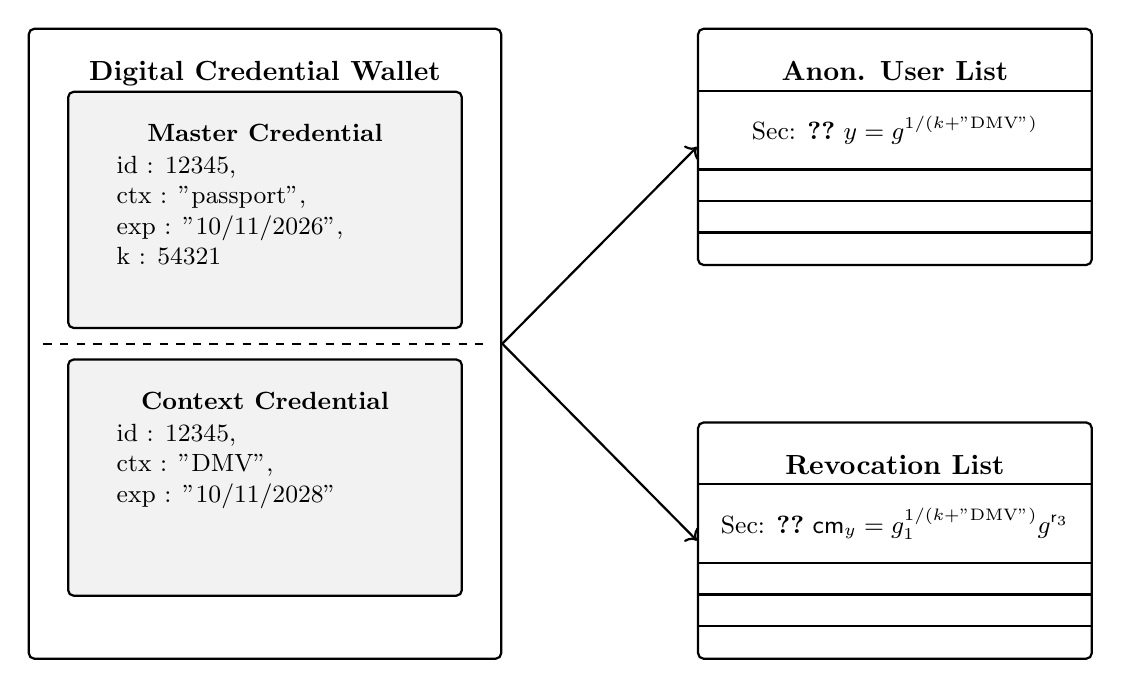
\begin{tikzpicture}[
        box/.style={draw, rounded corners=2pt, minimum width=6cm, minimum height=8cm},
        smallbox/.style={draw, rounded corners=2pt, fill=gray!10, minimum width=5cm, minimum height=3cm},
        listbox/.style={draw, rounded corners=2pt, minimum width=5cm, minimum height=3cm},
        thick
    ]
    
    % Digital Credential Wallet
    \node[box] (wallet) at (0,0) {};
    \node[anchor=north, font=\bfseries] at ($(wallet.north) + (0,-0.3)$) {Digital Credential Wallet};
    
    % Master Credential
    \node[smallbox] (master) at (0,1.7) {};
    \node[anchor=north, font=\small\bfseries] at ($(master.north) + (0,-0.3)$) {Master Credential};
    
    \node[anchor=north west, font=\small, align=left] at ($(master.north west) + (0.5,-0.7)$) {
        id : 12345, \\
        ctx : "passport", \\
        exp : "10/11/2026", \\
        k : 54321
    };
    
    % Context Credential
    \node[smallbox] (context) at (0,-1.7) {};
    \node[anchor=north, font=\small\bfseries] at ($(context.north) + (0,-0.3)$) {Context Credential};
    
    \node[anchor=north west, font=\small, align=left] at ($(context.north west) + (0.5,-0.7)$) {
        id : 12345, \\
        ctx : "DMV", \\
        exp : "10/11/2028"
    };
    
    % Add a dividing line between credentials in wallet
    \draw[dashed] ($(wallet.west) + (0.2,0)$) -- ($(wallet.east) + (-0.2,0)$);
    
    % Anonymous User List
    \node[listbox] (userlist) at (8,2.5) {};
    \node[anchor=north, font=\bfseries] at ($(userlist.north) + (0,-0.3)$) {Anon. User List};
    
    % Draw horizontal lines in the user list
    \draw ($(userlist.north west) + (0,-0.8)$) -- ($(userlist.north east) + (0,-0.8)$);
    
    % Formula in the second row of user list
    \node[font=\small, align=center] at ($(userlist.north) + (0,-1.3)$) {Sec: \ref{sec:privacy-preserving-vrf} $ y = g^{1/(k + \text{"DMV"})}$};
    
    \draw ($(userlist.north west) + (0,-1.8)$) -- ($(userlist.north east) + (0,-1.8)$);
    \draw ($(userlist.north west) + (0,-2.2)$) -- ($(userlist.north east) + (0,-2.2)$);
    \draw ($(userlist.north west) + (0,-2.6)$) -- ($(userlist.north east) + (0,-2.6)$);
    
    % Revocation List
    \node[listbox] (revlist) at (8,-2.5) {};
    \node[anchor=north, font=\bfseries] at ($(revlist.north) + (0,-0.3)$) {Revocation List};
    
    % Draw horizontal lines in the revocation list
    \draw ($(revlist.north west) + (0,-0.8)$) -- ($(revlist.north east) + (0,-0.8)$);
    
    % Formula in the second row of revocation list
    \node[font=\small, align=center] at ($(revlist.north) + (0,-1.3)$) {Sec: \ref{pok-committed-nullifier-vrf} $\cm_y = g_1^{1/(k + \text{"DMV"})}g^{\usk_3}$};

    
    
    \draw ($(revlist.north west) + (0,-1.8)$) -- ($(revlist.north east) + (0,-1.8)$);
    \draw ($(revlist.north west) + (0,-2.2)$) -- ($(revlist.north east) + (0,-2.2)$);
    \draw ($(revlist.north west) + (0,-2.6)$) -- ($(revlist.north east) + (0,-2.6)$);
    
    % Arrows - from wallet to lists, touching the boxes
    \draw[->, thick] (wallet.east) -- (userlist.west);
    \draw[->, thick] (wallet.east) -- (revlist.west);
    
    \end{tikzpicture}
    \caption{A credential hierarchy with nullifiers that bind context credentials to a master credential. The nullifiers create verifiable bindings that prevent sybil attacks while maintaining privacy, with separate paths for anonymous user authentication and revocation management.}
    \label{fig:credential-nullifier-revised}
\end{figure}


\subsection{Goals}


\begin{enumerate}
    \item \textbf{Efficiency}: The nullifier must be generated and verifiable with minimal overhead, avoiding bilinear pairings and MPC while maintaining provable uniqueness and verifiable pseudorandomness.
    
    \item \textbf{Anonymity}: Nullifier generation and verification must not reveal the user inputs $\k, \ctx$ and optionally enable unlinkable outputs. 
    
    \item \textbf{Integration with Anonymous Credentials}: The nullifier mechanism must seamlessly extend our existing anonymous credential framework without compromising its security properties.
\end{enumerate}

\subsection{Core Challenges}


Creating an efficient, privacy-preserving nullifier for credential binding raises three specific challenges:

\begin{enumerate}
    \item \textbf{Prime Order (Pairing-Free) DY VRF}: The DY VRF provides a secure structure but uses expensive bilinear pairings. Our first challenge is to create a Pairing-Free DY VRF using a $\Sigma$-protocol to maintain security under the $q$-DDHI assumption.
    
    \item \textbf{Anonymous Input for Prime-Order VRF}: To transform our Prime-Order DY VRF for Anonymous Credentials, we must use a commitment to the VRF inputs. Our second core challenge is to create a $\Sigma$-protocol to prove knowledge of $x$ such that $y = g^{1/x}$ (the $q$-DDHI challenge). Our third core challenge extends this by incorporating the proof of linear relations, the final protocol proves knowledge of $(x, sk)$ such that $y = g^{1/(sk + x)}$ where $y$ is a deterministic nullifier.
    
    \item \textbf{Unlinkable Output for Prime-Order VRF}: The deterministic nullifier can be used for sybil resistance during credential generation but can't be used ongoing as each output links the user's actions. Our fourth and last core challenge is to extend our protocol to generate provable, probabilistic nullifiers. We need to output a commitment to the nullifier so it can be used without linking the user. The final protocol proves knowledge of $(x, sk,r)$ such that $\cm_y = g_1^{1/(sk + x)}g^r$. 
\end{enumerate}



\subsection{Related Work}

\begin{table}
\begin{center}
\caption{Comparison of Nullifier/VRF Schemes for Credential Binding}
\label{tab:nullifier-comparison}
\begin{tabular}{l|cccccc}
\toprule
\textbf{Scheme} & 
\textbf{Deterministic} & 
\textbf{Unlinkable}  & 
\textbf{Private} & 
\textbf{Pairing-} & 
\textbf{Proof} & 
\textbf{Relative} \\
 & 
 \textbf{Output}$^1$ & 
 \textbf{Output}$^2$ & 
 \textbf{Input}$^3$ & 
 \textbf{Free} & 
 \textbf{Type} & 
 \textbf{Ver. Time}$^4$ \\
\midrule
NSEC5 \cite{goldberg_nsec5_2015} & 
\ding{51} & 
\ding{55} & 
\ding{55} & 
\ding{51} & 
Sigma Only & 3x faster
\\
DY VRF \cite{hutchison_verifiable_2005} & 
\ding{51} & 
\ding{55} & 
\ding{55} & 
\ding{55} & 
Pairing & 3x slower 
\\
CanDID \cite{maram2021candid} & 
\ding{51} & 
\ding{55} & 
\ding{51} & 
- & 
MPC & Very slow $^5$
\\
TACT/S3ID \cite{rabaninejad_attribute-based_2024} & 
\ding{51} & 
\ding{55} & 
\ding{51} & 
\ding{55} & 
Groth Sahai + Pairing & ~4x slower 
\\
SyRA \cite{crites_syra_2024} & 
\ding{51} & 
\ding{55} & 
\ding{55}  &
\ding{55} & 
 Sigma+Pairing & ~4x slower 
\\
UTT Nullifier \cite{tomescu2022utt} & 
\ding{51} & 
\ding{51} & 
\ding{51}  & 
\ding{55} & 
Sigma+Pairing & 4x slower 
\\
\text{Sec:} \ref{sec:privacy-preserving-vrf}: & 
\ding{51} & 
\ding{55} & 
\ding{51} & 
\ding{51} & 
Sigma only & 2x faster
\\
\text{Sec:} \ref{pok-committed-nullifier-vrf}: & 
\ding{51} & 
\ding{51} & 
\ding{51}  & 
\ding{51} & 
Sigma only & 1x (baseline) 
\\
\bottomrule
\end{tabular}
\end{center}
\vspace{1em}
\footnotesize{$^1$Ensures a unique underlying nullifier value per user-context pair for sybil resistance.} \\
\footnotesize{$^2$Nullifier can be presented as a commitment for unlinkability.} \\
\footnotesize{$^3$Operates on inputs (e.g., secret keys, attributes) hidden in commitments.} \\
\footnotesize{$^4$Approximate verification time relative to CRBN, based on benchmarks in Section \ref{sec:performance-vrf}} \\
\footnotesize{$^5$CanDIDs nullifier uses MPF{-}PRF with uncomparable efficiency}
\footnotesize{$^6$}
\end{table}

Previous systems have addressed aspects of hierarchical credential binding and sybil resistance, but all have significant limitations:

\begin{itemize}
    
    \item \textbf{Standard VRFs}~\cite{hutchison_verifiable_2005, goldberg_nsec5_2015} could generate unique nullifiers but use pairings and reveal the user's public key during verification, compromising anonymity.
        
    \item \textbf{Pairing-based systems} like SyRA~\cite{crites_syra_2024} and S3ID~\cite{rabaninejad_attribute-based_2024} implement hierarchical credentials but suffer from efficiency issues due to their reliance on pairings and S3ID uses Groth Sahai proofs which are less efficient than $\Sigma$-protocols.
    
    \item \textbf{UTT}~\cite{tomescu2022utt} uses a similar approach to ours for anonymous payments, creating serial numbers (nullifiers) from a registration credential. However, UTT relies on bilinear pairings, introducing substantial computational overhead.
    
    \item \textbf{CanDID}~\cite{maram2021candid} clearly defines the master/context credential relationship but compromises privacy by maintaining mappings between credential public keys, enabling linkability across interactions.

\end{itemize}


\subsection{Contributions}\label{sec:vrf-contributions}
We start with the $q$-DDHI assumption and work in two different directions. Firstly, we aim for efficiency and reconstruct the Dodis Yampolskiy VRF in a prime-order group and show XXX efficiency improvement while retaining security properties. Secondly, we aim for privacy,  starting with a novel zkpok protocol to prove the DDHI challenge $(g^{1/x})$ which we generalise to a sigma protocol for \emph{proof of inverse exponent}. We then extend this with a new private VRF to generate deterministic nullifiers from private inputs, combining our prime-order DY VRF and the ZKPoK of a DDHI challenge, where inputs are exponents in commitments for use in sybil-resistant mechanisms. We then extend this further for probabilistic outputs, committed but provable nullifiers to be used in revocation schemes. 


\begin{figure}[ht]
\centering
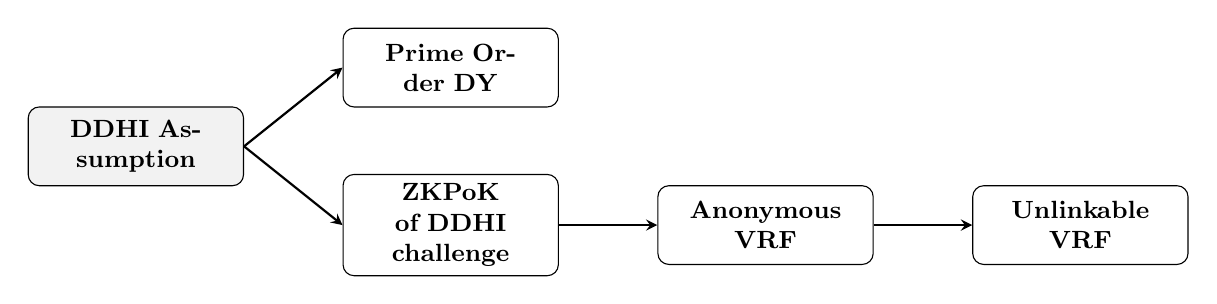
\begin{tikzpicture}[
    node distance=1cm,
    box/.style={rectangle, rounded corners, draw, fill=white, text width=2.5cm, minimum height=1cm, align=center, font=\small},
    arrow/.style={thick,->,>=stealth},
    improvement/.style={text width=3cm, align=center, font=\footnotesize\itshape}
]
% Root node
\node[box, fill=gray!10] (ddhi) {\textbf{DDHI Assumption}};

% Branch 1 - Top horizontal branch
\node[box, right=1.25cm of ddhi, yshift=1cm] (pfdy) {\textbf{Prime Order DY}};

% Branch 2 - Bottom horizontal branch with sequence
\node[box, right=1.25cm of ddhi, yshift=-1cm] (zkpok) {\textbf{ZKPoK of DDHI challenge}};
\node[box, right=1.25cm of zkpok] (anon) {\textbf{Anonymous VRF}};
\node[box, right=1.25cm of anon] (unlink) {\textbf{Unlinkable VRF}};

% Arrows between nodes with smooth curves
\draw[arrow] (ddhi.east) -- ++(0,0) -- (pfdy.west);
\draw[arrow] (ddhi.east) -- ++(0,0) -- (zkpok.west);
\draw[arrow] (zkpok.east) -- (anon.west);
\draw[arrow] (anon.east) -- (unlink.west);

% Improvement labels - positioned below the boxes
% \node[improvement, below=0.2cm of pfdy] {Remove Pairings};

% \node[improvement, below=0.2cm of zkpok] {Prove};
% \node[improvement, below=0.2cm of anon] {Adds privacy protection};
% \node[improvement, below=0.2cm of unlink] {Maintains verifiability while adding unlinkability};
\end{tikzpicture}
\caption{Sigma Protocols and VRF Constructions from the $q$-DDHI assumption}
\label{fig:vrf-construction-overview}
\end{figure}



\section{Preliminaries}

\subsection{Cryptographic Assumptions}

\begin{definition}[q-DDHI Assumption]
Let $\mathbb{G}$ be a cyclic group of prime order $p$ with generator $g$. The $q$-Decisional-Diffie-Hellman Inversion ($q$-DDHI) \cite{mitsunari_new_2002} assumption states that for any PPT adversary $\mathcal{A}$, there exists a negligible function $\negl$ such that:
\[
\left|\Pr\left[ x \sample \Zp^*, b \sample \{0,1\}, z_0 = g^{1/x}, z_1 \sample \G : \mathcal{A}(g, g^x, g^{x^2}, \ldots, g^{x^q}, z_b) = b \right] - \frac{1}{2}\right| \leq \negl(\lambda)
\]
Informally, given $(g, g^x, g^{x^2}, \ldots, g^{x^q})$, no PPT adversary can distinguish $g^{1/x}$ from a random group element with non-negligible advantage.
\end{definition}

% \begin{remark}
% The $q$-DDHI assumption is a variant of the $(q+1)$-generalized Diffie-Hellman assumption as shown by Boneh and Boyen \cite{kanade_efficient_2004}. This assumption directly underpins the security of our pairing-free VRF construction.
% \end{remark}

\begin{definition}[$q$-DBDHI Assumption]
Let $\mathbb{G}_1, \mathbb{G}_2, \mathbb{G}_T$ be cyclic groups of prime order $p$ with a bilinear pairing $e: \mathbb{G}_1 \times \mathbb{G}_2 \to \mathbb{G}_T$, and generators $g \in \mathbb{G}_1$, $\tilde{g} \in \mathbb{G}_2$. The $q$-Decisional-Bilinear Diffie-Hellman Inversion ($q$-DBDHI) assumption states that for any PPT adversary $\mathcal{A}$, there exists a negligible function $\negl$ such that:
\[
\left| \Pr\left[ x \sample \Z_p^*, b \sample \{0,1\}, z_0 = e(g, \tilde{g})^{1/x}, z_1 \sample \G_T : \mathcal{A}(g, g^x, g^{x^2}, \ldots, g^{x^q}, \tilde{g}, z_b) = b \right] - \frac{1}{2}\right| \leq \negl(\lambda)
\]
Informally, no PPT adversary can distinguish $e(g, \tilde{g})^{1/x}$ from a random element in $\mathbb{G}_T$ given $(g, g^x, \ldots, g^{x^q}, \tilde{g})$ with non-negligible advantage.
\end{definition}


\subsection{Building Blocks}

\subsubsection{Pedersen Vector Commitments}
We use position-binding Pedersen Commitments from Chapter 2, which allow committing to a vector of messages while hiding the values. For a message vector $[\id, \ctx, \exp, \k]$ and randomness $\usk$, the commitment is:
\[
\cm = \CMCom([m_1, \ldots, m_n];\usk) = g_1^{m_1} \cdots g_n^{m_n} g^\usk
\]

Pedersen Commitments provide three key properties:
\begin{itemize}
    \item \textbf{Hiding}: The commitment reveals no information about the committed values.
    \item \textbf{Binding}: It's computationally infeasible to open a commitment to different values.
    \item \textbf{Position-Binding}: Each position in the vector is cryptographically bound to its specific base element, preventing attribute swapping.
\end{itemize}


\subsubsection{Verifiable Random Functions}
A Verifiable Random Function (VRF) \cite{micali_verifiable_1999, hutchison_verifiable_2005} is a pseudorandom function that provides proofs of correct evaluation. Following \cite{bitansky_verifiable_2020}, a VRF consists of these algorithms:

\begin{definition}[Verifiable Random Function]
A VRF is a tuple of PPT algorithms \\
$(\VRFGen, \VRFEval, \VRFProve, \VRFVerify)$ with message space $\mathcal{X}$, output space $\mathcal{Y}$ and proof space $\Pi$ where:
\begin{itemize}
    \item $\VRFGen(1^\lambda) \to (sk, pk)$: Generates a secret key $sk$ and public key $pk$.
    \item $\VRFEval(sk,x) \to y$: Computes the VRF output $y \in \mathcal{Y}$ for input $x \in \mathcal{X}$ using secret key $sk$.
    \item $\VRFProve(sk,x) \to \pi$: Produces a proof $\pi \in \Pi$ that $y = \VRFEval(sk,x)$ is computed correctly.
    \item $\VRFVerify(pk,x,y,\pi) \to \{0,1\}$: Verifies that $y$ is the correct VRF output for input $x$ using proof $\pi$.
\end{itemize}
\end{definition}

A secure VRF must satisfy the following properties:

\begin{itemize}
    \item \textbf{Completeness:} Honest evaluation and proof generation always passes verification:
    \[
    \Pr\left[ \VRFVerify(pk,x,y,\pi) = 1 \ \middle| \ 
    \begin{array}{l}
        (sk, pk) \leftarrow \VRFGen(1^\lambda) \\
        y = \VRFEval(sk,x) \\
        \pi \leftarrow \VRFProve(sk,x)
    \end{array}
    \right] = 1
    \]
    
    \item \textbf{Uniqueness:} For each input $x$ and public key $pk$, only one output $y$ can be verified:
    \[
    \text{if} \quad \VRFVerify(pk, x, y_0, \pi_0) = \VRFVerify(pk, x, y_1, \pi_1) = 1 \quad \text{then} \quad y_0 = y_1
    \]
    
    \item \textbf{Pseudorandomness:} The VRF output is indistinguishable from random for any input not previously queried, defined by the following game $\mathcal{G}_{\mathcal{A}}^{\text{vrf}}$:
    \begin{enumerate}
        \item The VRF challenger samples $(sk, pk) \leftarrow \VRFGen(1^\lambda)$, and sends $pk$ to $\mathcal{A}$.
        \item $\mathcal{A}$ submits evaluation queries $x_1, \ldots, x_Q \in \mathcal{X}$, and receives $(y_i, \pi_i)$ for each query, where $y_i = \VRFEval(sk, x_i)$ and $\pi_i \leftarrow \VRFProve(sk, x_i)$.
        \item At any point, $\mathcal{A}$ submits a challenge input $x_* \in \mathcal{X}$ such that $x_* \not\in \{x_1, \ldots, x_Q\}$.
        \item The challenger computes $y_0^* = \VRFEval(sk, x_*)$, samples $y_1^* \sample \mathcal{Y}$ uniformly at random, then samples $b \sample \{0,1\}$ and sends $y_b^*$ to $\mathcal{A}$.
        \item $\mathcal{A}$ may continue to make evaluation queries for inputs other than $x_*$.
        \item At the end, $\mathcal{A}$ outputs a guess $b'$. The game outputs 1 if $b' = b$, and 0 otherwise.
    \end{enumerate}
    
    We say that the VRF satisfies pseudorandomness if for all PPT adversaries $\mathcal{A}$:
    \[
    \text{Adv}_{\mathcal{A}}^{\text{vrf}} := \left|\Pr\left[\mathcal{G}_{\mathcal{A}}^{\text{vrf}}(\lambda) = 1\right] - \frac{1}{2}\right| \leq \text{negl}(\lambda)
    \]
\end{itemize}


    
In our work, we focus on adapting the Dodis-Yampolskiy VRF \cite{hutchison_verifiable_2005}, which computes $y = e(g, \tilde{g})^{1/(sk+x)}$ in bilinear groups, to work efficiently in standard prime-order groups without pairings.

\begin{definition}[Dodis Yampolskiy VRF]
    The Dodis-Yampolskiy (DY) VRF~\cite{hutchison_verifiable_2005} operates in a bilinear group setting with groups $\mathbb{G}_1$, $\mathbb{G}_2$, and $\mathbb{G}_T$ of prime order $p$, and a Type-3 pairing $e: \mathbb{G}_1 \times \mathbb{G}_2 \to \mathbb{G}_T$. Let $g \in \mathbb{G}_1$ and $\tilde{g} \in \mathbb{G}_2$ be generators. The VRF is defined as:

\begin{itemize}
    \item $\mathsf{VRF.Gen}(1^\lambda)$: Sample $sk \sample \mathbb{Z}_p^*$, set $pk = g^{sk}$.
    \item $\mathsf{VRF.Eval}(sk, x)$: Compute $y = e(g, \tilde{g})^{1/(sk + x)}$.
    \item $\mathsf{VRF.Prove}(sk, x)$: Compute $\pi = \tilde{g}^{1/(sk + x)}$.
    \item $\mathsf{VRF.Vfy}(pk, x, y, \pi)$: Check $e(g^{x} \cdot pk, \pi) \stackrel{?}{=} e(g, \tilde{g})$ and $y \stackrel{?}{=} e(g, \pi)$.
\end{itemize}

Security relies on the $q$-DBDHI assumption, ensuring $y$ is pseudorandom.

\end{definition}



\subsubsection{Zero-Knowledge Proofs and Sigma-Protocols}
Our credential binding mechanism relies on zero-knowledge proofs, particularly Sigma-protocols, to verify relations between committed values without revealing them.

A Sigma-protocol is a three-move interactive proof system where:
\begin{enumerate}
    \item The prover $\mathcal{P}$ sends a commitment message $a$.
    \item The verifier $\mathcal{V}$ sends a random challenge $e$.
    \item The prover responds with $z$, and $\mathcal{V}$ accepts if the verification equation holds.
\end{enumerate}
These protocols satisfy:
\begin{itemize}
    \item \textbf{Completeness}: For all $(x,w) \in \mathcal{R}$, an honest prover always convinces the verifier.
    \item \textbf{Special Soundness}: There exists an efficient extractor $\mathcal{E}$ such that, given any statement $x$ and two accepting transcripts $(a,e,z)$ and $(a,e',z')$ with $e \neq e'$, $\mathcal{E}$ can extract a witness $w$ such that $(x,w) \in \mathcal{R}$.
    \item \textbf{Special Honest-Verifier Zero-Knowledge}: There exists an efficient simulator $\mathcal{S}$ that, given a statement $x$ and a challenge $e$, produces a transcript $(a,e,z)$ that is computationally indistinguishable from a real transcript between an honest prover and verifier, without using a witness.
\end{itemize}












\section{Prime-Order VRF from the q-DDHI Assumption}\label{sec:pairing-free-vrf}

The Dodis-Yampolskiy \cite{hutchison_verifiable_2005} VRF provides an elegant solution for generating unique, pseudorandom nullifiers $y$ and their proofs of correctness $\pi$. We start with the question of removing pairings to improve efficiency. DY consists of $(y, \pi)$:
\[
y = e(g, \tilde{g})^{1/(sk+x)} \qquad \pi = \tilde{g}^{1/(sk+x)}
\]

Verification depends on the bilinearity property $e(g^a, \tilde{g}^b)^c = e(g, \tilde{g})^{abc}$, which enables "exponent multiplication" across groups, allowing the transformations:

\begin{align*}
    \begin{array}{rcl}
    e(g^x \cdot pk, \pi) & \stackrel{?}{=} & e(g^{sk+x}, \tilde{g}^{1/(sk+x)}) \\
     & \stackrel{?}{=} & e(g, \tilde{g})^{(sk+x)/(sk+x)} \\
     & = & e(g, \tilde{g})
    \end{array}
    &&
    \begin{array}{rcl}
    y & \stackrel{?}{=} & e(g, \pi) \\
     & \stackrel{?}{=} & e(g,\tilde{g}^{1/(sk+x)}) \\
     & = & e(g, \tilde{g})^{1/(sk+x)}
    \end{array}
\end{align*}

Security relies on the $q$-DBDHI problem which states that given $(g, g^x, g^{x^2}, \ldots, g^{x^q}, \tilde{g})$, no $\PPT$ adversary can distinguish between $e(g,\tilde{g})^{1/x}$ and a uniform element in $\G_T$ with non-negligible advantage , ensuring the VRF outputs maintain pseudorandomness after the adversary has observed $(x',y',\pi')$ pairs.

\subsubsection{The Prime-Order Group Challenge}

Prime-order groups and standard group operations (without such bilinearity property) cannot be used to directly verify the $1/(sk+x)$ relationship with standard cryptographic operations. For example, given $pk  \cdot g^x = g^{sk+x}$, verification attempts to equate or cancel out fail:

\begin{enumerate}
    \item $g^{sk+x} \cdot g^{1/(sk+x)} = g^{sk + x + \frac{1}{sk+x}}$
    \item $\frac{g^{sk+x}}{g^{1/(sk+x)}} = g^{(sk+x)^2-\frac{1}{sk+x}}$
\end{enumerate}

Our insight is to reverse the verification approach. Instead of trying to derive $g^{1/(sk+x)}$ from $g^{sk+x}$ or cancel with a reciprocal, we use a zero knowledge proof $\Sigma$-protocol to verify that $y$ raised to the power $(sk+x)$ equals $g$. In doing so, our pairing-free construction shifts from the $q$-DBDHI assumption to the $q$-DDHI assumption. This gives us the relation:

\[
\mathcal{R}_{\mathsf{DY-PF}} = \left\{ 
\begin{array}{l} 
(\pk, x, y),\\
(sk) 
\end{array}
\ \middle|
\ \begin{array}{l}
pk = g^{sk} \\
y^{sk + x} = g  \\
\end{array} \right\}
\]

\subsection{Construction}\label{sec-dy-pf}

Our VRF operates in a prime-order group $\mathbb{G}$ of order $p$ with generator $g$. The message space is $\mathcal{X} = \mathbb{Z}_p$, the output space is $\mathcal{Y} = \mathbb{G}$, and the proof space is $\Pi = \mathbb{G} \times \mathbb{G} \times \mathbb{Z}_p$. The algorithms are defined as follows:

\begin{itemize}
    \item $\mathsf{VRF.Gen}(1^\lambda) \to (sk, pk)$: Sample $sk \sample \mathbb{Z}_p^*$, compute $pk = g^{sk}$, and output $(sk, pk)$.
    \item $\mathsf{VRF.Eval}(sk, x) \to y$: Compute $y = g^{1/(sk + x)} \in \mathbb{G}$.
    \item $\mathsf{VRF.Prove}(sk, x) \to \pi$: Generate proof $\pi$ using the $\Sigma$-protocol described below.
    \item $\mathsf{VRF.Verify}(pk, x, y, \pi) \to \{0, 1\}$: Output 1 if $\pi$ verifies $y$ correctly per the $\Sigma$-protocol, else 0.
\end{itemize}

\begin{remark}
    Verifying $\VRFVerify(pk, x, \VRFEval(sk, x) \to y) \to 1$ is a naive verification approach without a proof which yeilds a Verifiable Unpredictable Function (VUF), not a VRF because it lacks the mechanism to prove pseudorandomness to a verifier. DY uses pairings to bridge the gap, we replace pairings with a $\Sigma$-protocol. 
\end{remark}

\subsection{Proof Protocol}
\begin{protocol}{DY Prime Order Proof Protocol}{}\label{protocol-pdy-protocol1}
\textbf{Common Input:} $g, pk, y \in \mathbb{G}$, $x \in \mathbb{Z}_p$ \\
\textbf{Prover Input:} $sk \in \mathbb{Z}_p^*$ with $pk = g^{sk}$, $y = g^{1/(sk + x)}$ \\
\textbf{Relation: }
\[
\mathcal{R} = \left\{ (\pk, x, y), (sk) \ \middle| pk = g^{sk} \land y^{sk + x} = g \right\}
\]
\begin{enumerate}
    \item \textbf{Commitment:} Prover samples $r \sample  \mathbb{Z}_p$, computes $T_1 = g^r$, $T_2 = y^r$, sends $(T_1, T_2)$.
    \item \textbf{Challenge:} Verifier samples $c \sample  \mathbb{Z}_p$, sends $c$.
    \item \textbf{Response:} Prover computes $z = r + c \cdot (sk + x)$, sends $z$.
    \item \textbf{Verification:} Verifier checks: $g^z \stackrel{?}{=} T_1 \cdot (pk \cdot g^x)^c$ and $y^z \stackrel{?}{=} T_2 \cdot g^c$
\end{enumerate}
\end{protocol}

\subsection{Security Analysis}

Our construction replaces the stronger information-theoretic uniqueness of DY VRF with (weaker) computational uniqueness via the $\Sigma$-protocol and discrete logarithm assumption.


\subsubsection{Correctness}

Correctness requires that an honest prover’s output $y$ and proof $\pi$ always pass verification. For $pk = g^{sk}$, $y = g^{1/(sk + x)}$, $T_1 = g^r$, $T_2 = y^r$, and $z = r + c(sk + x)$, the verification equations hold:
\begin{align*}
g^z &= g^{r + c(sk + x)} = g^r \cdot g^{c(sk + x)} = g^r \cdot (g^{sk} \cdot g^x)^c = T_1 \cdot (pk \cdot g^x)^c \\
y^z &= y^{r + c(sk + x)} = y^r \cdot y^{c(sk + x)} = y^r \cdot (y^{sk + x})^c = y^r \cdot g^c = T_2 \cdot g^c
\end{align*}

Since $y^{sk + x} = g^{1/(sk + x) \cdot (sk + x)} = g$, both checks pass, confirming correctness.

\subsubsection{Uniqueness}

Uniqueness ensures that, for a fixed $pk$ and $x$, only one $y$ can be successfully verified. In DY, pairings enforce this information theoretically. In P-DY, uniqueness is computational, relying on the discrete logarithm problem.

For a valid $y$, $y^{sk + x} = g$, so $y = g^{1/(sk + x)}$ is unique in $\mathbb{G}$. Suppose an adversary produces $y' \neq y$ with a valid proof $\pi'$. Then $y'^{sk + x} = g$ and $y^{sk + x} = g$, implying $(y'/y)^{sk + x} = 1$. In a prime-order group, $y'/y = g^k$ for some $k \neq 0$, so $y' = y \cdot g^k$. But $y'^{sk + x} = (y \cdot g^k)^{sk + x} = g \cdot g^{k(sk + x)} = g$ requires $g^{k(sk + x)} = 1$, which holds only if $k(sk + x) = 0 \pmod{p}$. For random $sk$ and $x$, $sk + x = 0$ is negligible. Alternatively, if $y'$ corresponds to a different $sk'$ where $pk = g^{sk'}$, finding $sk' \neq sk$ breaks the discrete logarithm assumption.

Thus, producing a distinct verifiable $y'$ is computationally infeasible, ensuring uniqueness.

\subsubsection{Pseudorandomness}

Pseudorandomness requires that $y = g^{1/(sk + x)}$ appears random in $\mathbb{G}$ without knowledge of $sk$, even given other input-output pairs. We rely on the $q$-DDHI assumption, which states that $g^{1/(sk + x)}$ is indistinguishable from random given $(g, g^{sk}, \ldots, g^{(sk)^q})$ for polynomial $q$. 
The $\Sigma$-protocol is zero-knowledge, leaking no information about $sk$ beyond $pk$.

\begin{proof}[Sketch]
    Assume an adversary can distinguish $y$ from random, solving $q$-DDHI. The challenger simulates proofs for $q$ inputs using $g^{sk^i}$ for challenge $x^*$, provides $y^* = g^{a/(sk + x^*)}$ or a random element. A successful distinguished implies a $q$-DDHI solver which is assumed to be a hard problem.
\end{proof}










\section{Anonymous Prime-Order VRFs from the $q$-DDHI}\label{sec:privacy-preserving-vrf}

While our pairing-free VRF construction, presented in Section 3, eliminates the computational overhead of bilinear pairings, it still exposes the public key $pk = g^{sk}$ and input $x$ during verification. This is a limitation for anonymous credential systems, where both the master credential key $sk$ and the context identifier $x$ must remain private to ensure user anonymity. In this section, we address this challenge by developing zero-knowledge proof techniques that enable verification of VRF outputs computed from committed attributes, without revealing sensitive information.

Our approach builds progressively across three key stages:

\begin{enumerate}
    \item \textbf{Proving Knowledge of a Committed Inverse Exponent}: We start with a foundational protocol to prove that a value $y = g^{1/x}$ corresponds to a committed exponent $x$, leveraging the $q$-DDHI assumption. This establishes the base for our next protocols.

    \item \textbf{Proving Knowledge of a Committed Inverse Linear Relation}: We extend this technique to handle linear combinations of committed values, enabling verification of a VRF output $y = g^{1/(sk + x)}$ where $sk$ and $x$ are committed in separate credentials. This deterministic nullifier supports privacy-preserving credential binding and sybil resistance.

    \item \textbf{Proving Knowledge of a Committed Nullifier}: Finally, we introduce a protocol to commit to the VRF output itself (i.e., $\cm_y = g_3^{1/(sk + x)} g^{r_3}$), allowing unlinkable presentations. This probabilistic nullifier ensures that repeated uses of the same credential relationship remain unlinkable while still verifiable.
\end{enumerate}

These protocols collectively transform our prime-order VRF into a privacy-preserving tool suitable for hierarchical anonymous credential systems. In the subsections that follow, we detail each stage, presenting the cryptographic constructions and their security properties. \ref{sec-instantiation} will later demonstrate how these building blocks are instantiated for sybil resistance and revocation in the Multi-Issuer Multi-Credential (MIMC) system.














\subsection{Proving Knowledge of a Committed Inverse Exponent}

The central challenge in constructing a pairing-free VRF lies in verifying the correctness of an inverse relationship, specifically that $y = g^{1/x}$ for committed values, without relying on bilinear pairings. In standard prime-order group cryptography, while computing $g^x$ is straightforward, directly verifying $g^{1/x}$ is not, as pairings typically enable this through $e(g^x, g^{1/x}) = e(g,g)$. Our key insight is to reformulate this verification by proving an equivalent relationship: $y^x = g$. This equivalence holds because if $y = g^{1/x}$, then $y^x = (g^{1/x})^x = g^{(1/x) \cdot x} = g$, and conversely, if $y^x = g$, then $y = g^{1/x}$ (assuming $x \neq 0 \mod q$). This transformation eliminates the need for pairings by enabling verification via standard exponentiation, which can be efficiently proven using zero-knowledge techniques.

The protocol we present leverages this equivalence through a zero-knowledge proof where the prover demonstrates knowledge of the opening of a commitment $\cm = g_1^x g^r$ while simultaneously proving that $y^x = g$. This dual verification ensures that $y$ correctly encodes the inverse of $x$ without revealing $x$, forming a foundation for our pairing-free VRF that balances efficiency and privacy.


\subsubsection{Construction}

We begin with a simplified relation: given a commitment $\cm = g_1^x g^r$ and an element $y = g^{1/x}$, the prover demonstrates knowledge of $x$ and $r$ satisfying both equations, without revealing them. This is linked to the Decisional Diffie-Hellman Inversion (DDHI) assumption—where distinguishing $g^{1/x}$ from a random element given $g, g^x$ is computationally hard—making it a secure and essential starting point for our privacy-preserving construction.


\begin{protocol}{Proving Knowledge of Inverse Exponent}{committed-inverse-exponent}\label{pok-committed-inverse-exponent}
\textbf{Common Input:} Group generators $g_1, g \in \mathbb{G}$, commitment $\cm \in \mathbb{G}$, and element $y \in \mathbb{G}$ \\
\textbf{Prover Input:} Witness $(x, r)$ such that $\cm = g_1^x g^r$ and $y = g^{1/x}$ \\
\textbf{Relation:} 
\[
\mathcal{R} = \left\{ (\cm, y), (x, r) \ \middle|\ \cm = g_1^x g^r \ \land\ y = g^{1/x} \right\}
\]
\begin{enumerate}
    \item \textbf{Commitment:} Prover samples $a_x, a_r \sample \mathbb{Z}_q$ and computes:
    \[
    T_1 = g_1^{a_x} g^{a_r}, \quad T_y = y^{a_x}
    \]
    Sends $(T_1, T_y)$ to the verifier.

    \item \textbf{Challenge:} Verifier samples $c  \sample  \mathbb{Z}_q$ and sends $c$ to the prover.

    \item \textbf{Response:} Prover computes:
    \[
    z_x = a_x + c \cdot x, \quad z_r = a_r + c \cdot r
    \]
    Sends $(z_x, z_r)$ to the verifier.

    \item \textbf{Verification:} Verifier checks:
    \[
    T_1 \cdot \cm^c \stackrel{?}{=} g_1^{z_x} g^{z_r}, \quad T_y \cdot g^c \stackrel{?}{=} y^{z_x}
    \]
\end{enumerate}
\end{protocol}



This protocol achieves two objectives simultaneously:
\begin{enumerate}
    \item The first verification equation ($T_1 \cdot \cm^c \stackrel{?}{=} g_1^{z_x} g^{z_r}$) proves the prover knows a valid opening $(x, r)$ of the commitment $\cm$. This is a standard Schnorr-type proof for Pedersen commitments.
    
    \item The second equation ($T_y \cdot g^c \stackrel{?}{=} y^{z_x}$) verifies that $y^x = g$, which means $y = g^{1/x}$. This is the critical link proving that $y$ is correctly computed as the inverse exponent.
\end{enumerate}


\subsubsection{Security Analysis}

The protocol satisfies the standard security properties of Sigma protocols: completeness, special soundness, and honest-verifier zero-knowledge.

\paragraph{Completeness.} For an honest prover with witness $(x, r)$ satisfying $\cm = g_1^x g^r$ and $y = g^{1/x}$, the verification equations hold as demonstrated in the protocol~\ref{pok-committed-inverse-exponent}.

\paragraph{Special Soundness.} Given two accepting transcripts with different challenges, an extractor $\mathcal{E}$ can compute $x = \frac{z_x - z_x'}{c - c'}$ and $r = \frac{z_r - z_r'}{c - c'}$. The extracted values satisfy both $\cm = g_1^x g^r$ and $y^x = g$, confirming $y = g^{1/x}$.

\paragraph{Honest-Verifier Zero-Knowledge.} There exists a simulator $\mathcal{S}$ that, given only the statement $(\cm, y)$ and a challenge $c$, produces transcripts indistinguishable from real protocol executions by sampling $z_x, z_r \sample \mathbb{Z}_p$ and computing commitment values that satisfy the verification equations.

Detailed proofs of these properties are provided in Appendix~\ref{app:vrf-committed-inverse-exponent}.


\paragraph{Relation to $q$-DDHI Assumption.}  The $q$-DDHI assumption ensures that $g^{1/x}$ is computationally indistinguishable from random elements when $x$ is hidden. However, pseudorandomness requires outputs remain indistinguishable even after seeing multiple input-output pairs from the same secret key, and therefore $y = g^{1/x}$ is not pseudorandom.





























\subsection{Proving Knowledge of a Committed Inverse Linear Relation}

We then extend this to prove a linear relation of inverse exponents $y = g^{1/(sk+x)}$ where $sk$ and $x$ come from different commitments, enforcing a relation $\mathcal{R}_{\mathsf{nullifier}}$ holds. We show the full protocol here \ref{pok-committed-inverse-linear-relation}. 

\[
\mathcal{R}_{\mathsf{nullifier}} = \left\{ 
\begin{array}{l} (\cm_1, \cm_2, y),\\
(sk, x, r_1, r_2) 
\end{array}
\ \middle|
\ \begin{array}{l}
\cm_1 = g_1^{sk} g^{r_1} \\
\cm_2 = g_2^{x} g^{r_2} \\
y = g^{1/(sk + x)} \\
\end{array} \right\}
\]






\subsubsection{Construction}

We now extend our approach to handle linear combinations of committed values. Given commitments $\cm_1 = g_1^{sk} g^{r_1}$ and $\cm_2 = g_2^{x} g^{r_2}$ to values $sk$ and $x$, we want to prove that $y = g^{1/(sk + x)}$ without revealing $sk$, $x$, or the randomness values.

This extension is essential for the credential binding scenario, where $sk$ is a secret key in a master credential and $x$ is a context identifier in a separate credential. The protocol must verify the correct computation of $y$ from these disparate committed values.

\begin{protocol}{Proving Committed Inverse Linear Relation}{}\label{pok-committed-inverse-linear-relation}
\textbf{Common Input:} Group generators $g_1, g_2, g \in \mathbb{G}$, $\cm_1, \cm_2, y \in \mathbb{G}$ \\
\textbf{Prover Input:} Witness $(sk, x, \usk_1, \usk_2)$ such that $\cm_1 = g_1^{sk} g^{\usk_1}$, $\cm_2 = g_2^{x}g^{\usk_2}$ and $ y = g^{1/(sk + x)}$ \\
\textbf{Relation: }
\[
\mathcal{R} = \{(\cm_1,\cm_2, y), (sk, x, \usk_1, \usk_2) \mid \cm_1 = g_1^{sk} g^{\usk} \wedge \cm_2 = g_2^{x}g^{\usk_2} \wedge y = g^{1/(sk + x)}\}
\]
\begin{enumerate}
    \item \textbf{Commitment:} Prover computes:
    \begin{align*}
        a_{sk}, a_x, a_{r_1}, a_{r_2} &\sample \Z_q & T_1 &\gets g_1^{a_{sk}} g^{a_{r_1}} & T_2 &\gets g_2^{a_x} g^{a_{r_2}} & T_y &\gets y^{a_{sk} + a_x}
    \end{align*}
    Sends $(T_1, T_2, T_y)$ to verifier.
    
    \item \textbf{Challenge:} Verifier samples $c \sample \mathbb{Z}_q$ and sends to prover.
    
    \item \textbf{Response:} Prover computes:
     \begin{align*}
        z_{sk} &= a_{sk} + c \cdot sk & z_x &= a_x + c \cdot x &  z_m &= (a_{sk} + a_x) + c \cdot (sk + x)\\   
        z_{r_1} &= a_{r_1} + c \cdot r_1 & z_{r_2} &= a_{r_2} + c \cdot r_2
    \end{align*}
    Sends $(z_{sk}, z_x, z_{r_1} z_{r_2}, z_m)$ to verifier.
    
    \item \textbf{Verification:} Verifier checks:
    \begin{align*}
        T_1 \cdot \cm_1^c &\stackrel{?}{=} g_1^{z_{sk}}g^{z_{r_1}} 
        &
        T_2 \cdot \cm_2^c &\stackrel{?}{=}  g_2^{z_x} g^{z_{r_2}} 
        &
        T_y \cdot g^c &\stackrel{?}{=} y^{z_m} &
        z_m &\stackrel{?}{=} z_{sk} + z_x
    \end{align*}
\end{enumerate}
\end{protocol}


This protocol extends our basic approach in two key ways:
\begin{enumerate}
    \item It simultaneously proves knowledge of openings for two separate commitments ($\cm_1$ and $\cm_2$).
    \item It verifies that $y^{sk+x} = g$, proving $y = g^{1/(sk+x)}$, where the exponent $sk+x$ is a linear combination of values from different commitments.
\end{enumerate}

The additional check $z_m \stackrel{?}{=} z_{sk} + z_x$ ensures consistency between the individual responses and their sum, preventing a malicious prover from using different values in different parts of the proof.

\subsubsection{Security Analysis}

The security analysis follows similar principles to the basic protocol, with the additional complexity of handling two commitments and their linear combination.

\paragraph{Completeness:} For an honest prover, all verification equations hold by similar derivations to the basic case, with the additional consistency check $z_m = z_{sk} + z_x$ holding by construction.

\paragraph{Special Soundness:} Given two accepting transcripts with different challenges, we can extract $sk$, $x$, $r_1$, and $r_2$ satisfying the commitment openings and, crucially, verify through the third equation that $y^{sk+x} = g$, proving $y = g^{1/(sk+x)}$.

\paragraph{Honest-Verifier Zero-Knowledge:} A simulator can generate indistinguishable transcripts by sampling responses randomly and computing commitments that satisfy the verification equations, ensuring no information about the witness is revealed.

This protocol forms the foundation for our credential binding nullifier, allowing us to prove relationships between attributes from different credentials without compromising privacy.





































\subsection{Proving Knowledge of a Committed Nullifier}

A deterministic nullifier $y = g^{1/(sk+x)}$ is necessary for Sybil resistance ensuring a unique, verifiable value for each $(sk,x)$ pair. However, deterministic algorithms create privacy problems with linkability. There are many use-cases for the verifiable connection of $(sk, x)$, such as revocation accumulators, which a user would need to interact with frequently, requiring a probabilistic output that can verify the $(sk+x)$ connection. 

Our solution is to commit to the nullifier rather than revealing it directly:
\[
\cm_{\mathsf{null}} = g_3^{1/(sk+x)} g^{r_3}
\]

We must now prove that the committed value represents the nullifiers $(sk+x)$, we do so with the following relation:


\[
\mathcal{R}_{\mathsf{CommittedNull}} = \left\{ 
\begin{array}{l} 
(\cm_1, \cm_2, \cm_3, \cm_4), \\
(sk, x, r_1, r_2, r_3, r_4) 
\end{array}
\ \middle| \
\begin{array}{l}
\cm_1 = g_1^{sk} g^{r_1} \\
\cm_2 = g_2^{x} g^{r_2} \\
\cm_3 = g_3^{1/(sk + x)} g^{r_3}  \quad \text{\small{The Committed Nullifier}}\\
\cm_4 = \cm_3^{sk + x} g^{r_4} = g_3 g^{r_3 (sk + x) + r_4}
\end{array} \right\}
\]

The auxiliary commitment $\cm_4$ enables verification analogous to our approach in Challenge 1: instead of verifying $y^{sk+x} = g$ directly, we prove that $\cm_3^{sk+x} = g_3$ (modulo some randomness $g^{r_4}$). This algebraic relationship can only hold if $\cm_3$ commits to $g_3^{1/(sk+x)}$, thus verifying the correctness of the committed nullifier without revealing it.

This construction extends our technique from Challenge 2 by applying the exponentiation-inversion verification paradigm entirely within the commitment space. The verification operates on the same mathematical principle ($x \cdot \frac{1}{x} = 1$), but now uses homomorphic properties of Pedersen commitments to prove the relationship between committed values, enabling both unlinkable presentations and verifiable credential binding.



\subsubsection{Construction}\label{sec:committed-nullifier}


In the Multi-Issuer Multi-Credential Attribute-Based Anonymous Credential (MIMC-ABC) system, nullifiers ensure sybil resistance by enforcing uniqueness of context-specific credentials bound to a master credential. However, exposing nullifiers as public values, as in our pairing-free Verifiable Random Function (VRF) construction (Section~\ref{sec-dy-pf}), risks linkability across presentations, compromising user privacy. To address this, we propose a novel zero-knowledge protocol that commits the nullifier within a Pedersen commitment, proving its correctness relative to committed attributes from master and context credentials without revealing sensitive information.

Our goal is to design a Sigma-protocol that proves a commitment $\cm_3 = g_3^{1/(sk + x)} g^{r_3}$ contains the inverse exponent $1/(sk + x)$, where $sk$ and $x$ are attributes committed in $\cm_1 = g_1^{sk} g^{r_1}$ (master credential) and $\cm_2 = g_2^{x} g^{r_2}$ (context credential), respectively. This enables privacy-preserving sybil resistance, allowing nullifiers to be used in applications like set membership proofs without linking user actions. The protocol operates in prime-order groups, avoiding the computational overhead of bilinear pairings, and integrates seamlessly with MIMC-ABC's efficient Sigma-protocol framework.

The novelty of our approach lies in its pairing-free, zero-knowledge proof of a committed inverse linear relation, a significant advancement over prior VRF-based nullifiers that rely on pairings or expose inputs \cite{hutchison_verifiable_2005,tomescu2022utt}. By committing the nullifier, we achieve unlinkability, a critical requirement for anonymous credential systems in regulatory contexts like KYC/AML. Furthermore, our protocol is 33\% faster in evaluation and 60\% faster in verification compared to pairing-based schemes (Section~\ref{sec:performance}), offering practical scalability for real-world deployments.

This contribution is crucial for enabling hierarchical, sybil-resistant anonymous credentials that balance privacy, accountability, and efficiency. It addresses practical challenges in federated identity systems, where users must prove credential relationships without compromising anonymity, and lays the foundation for advanced functionalities like private revocation and accumulator-based proofs.

\begin{protocol}{Proving Committed Nullifier for VRF}{committed-nullifier-vrf}\label{pok-committed-nullifier-vrf}
\textbf{Common Input:} Group generators $g_1, g_2, g_3, g \in \mathbb{G}$, commitments $\cm_1, \cm_2, \cm_3, \cm_4 \in \mathbb{G}$ \\
\textbf{Prover Input:} Witness $(sk, x, r_1, r_2, r_3, r_4)$ such that:
    \[
    \cm_1 = g_1^{sk} g^{r_1}, \quad \cm_2 = g_2^{x} g^{r_2}, \quad \cm_3 = g_3^{1/(sk + x)} g^{r_3}, \quad \cm_4 = \cm_3^{sk + x} g^{r_4} = g_3 g^{r_3 (sk + x) + r_4}
    \]
\textbf{Relation:}
\[
\mathcal{R} = \left\{ 
\begin{array}{l} 
(\cm_1, \cm_2, \cm_3, \cm_4), \\
(sk, x, r_1, r_2, r_3, r_4) 
\end{array}
\ \middle| \
\begin{array}{l}
\cm_1 = g_1^{sk} g^{r_1} \\
\cm_2 = g_2^{x} g^{r_2} \\
\cm_3 = g_3^{1/(sk + x)} g^{r_3} \\
\cm_4 = \cm_3^{sk + x} g^{r_4} = g_3 g^{r_3 (sk + x) + r_4}
\end{array} \right\}
\]
\begin{enumerate}
    \item \textbf{Commitment:} Prover samples $a_{sk}, a_x, a_{r_1}, a_{r_2}, a_{r_3}, a_{r_4} \sample \mathbb{Z}_q$ and computes:
       \[
       T_1 = g_1^{a_{sk}} g^{a_{r_1}}, \quad T_2 = g_2^{a_x} g^{a_{r_2}}, \quad T_3 = g_3^{a_{\beta}} g^{a_{r_3}}, \quad T_4 = \cm_3^{a_{sk} + a_x} g^{a_{r_4}}
       \]
       where $a_{\beta} = 1/(a_{sk} + a_x)$. Sends $(T_1, T_2, T_3, T_4)$ to verifier.
    
    \item \textbf{Challenge:} Verifier samples $c \sample \mathbb{Z}_q$ and sends to prover.
    
    \item \textbf{Response:} Prover computes:
       \[
       z_{sk} = a_{sk} + c \cdot sk, \quad z_x = a_x + c \cdot x, \quad z_{r_1} = a_{r_1} + c \cdot r_1, \quad z_{r_2} = a_{r_2} + c \cdot r_2
       \]
       \[
       z_{r_3} = a_{r_3} + c \cdot r_3, \quad z_{r_4} = a_{r_4} + c \cdot r_4
       \]
       Sends $(z_{sk}, z_x, z_{r_1}, z_{r_2}, z_{r_3}, z_{r_4})$ to verifier.
    
    \item \textbf{Verification:} Verifier checks:
       \[
       T_1 \cdot \cm_1^c \stackrel{?}{=} g_1^{z_{sk}} g^{z_{r_1}}, \quad T_2 \cdot \cm_2^c \stackrel{?}{=} g_2^{z_x} g^{z_{r_2}}, \quad T_3 \cdot \cm_3^c \stackrel{?}{=} g_3^{z_{\beta}} g^{z_{r_3}}
       \]
       \[
       T_4 \cdot \cm_4^c \stackrel{?}{=} \cm_3^{z_{sk} + z_x} g^{z_{r_4}}
       % \cm_4 \stackrel{?}{=} g_3 g^{s} \text{ for some } s \in \mathbb{Z}_q
       \]
\end{enumerate}
\end{protocol}


\subsubsection{Security Analysis}












\section{Performance Evaluation}\label{sec:performance-vrf}

We implemented our constructions \cite{polgar_anonymous_2025} using the arkworks cryptography library \cite{arkworks_contributors_arkworks_2022} in Rust and evaluated performance on a MacBook Air M2 with 16GB RAM. Table~\ref{tab:performance-vrf} compares our constructions on BLS12-381 curve against baseline approaches, focusing on the critical operations of evaluation, proof generation, and verification. Table \ref{tab:performance-vrf-curves} shows our constructions built on different, non-pairing curves.

\begin{table}[ht]
\begin{center}
\caption{VRF Comparison with curve BLS12-381}
\label{tab:performance-vrf}
\begin{tabular}{l@{\hspace{1em}}c@{\hspace{1em}}r@{\hspace{2em}}r@{\hspace{5em}}r@{\hspace{2em}}r}
\toprule
\textbf{Scheme} & \textbf{Pairing} & \multicolumn{2}{c}{\textbf{Eval + Prove (ms)}} & \multicolumn{2}{c}{\textbf{Verify (ms)}} \\
\cmidrule(lr){3-4} \cmidrule(lr){5-6}
& & \textbf{ms} & \textbf{Speedup} & \textbf{ms} & \textbf{Speedup} \\
\midrule
DY$^1$ \cite{hutchison_verifiable_2005}                     & yes & 1.27 &  -      & 2.2   &  -     \\
Our DY-PF \ref{sec-dy-pf}                                   & no  & 0.41 & 3.1x   & 0.70  & 3.1x  \\
\midrule
DY Private \cite{tomescu2022utt}                            & yes & 5.91 &   -     & 6.47  &   -    \\
Our DY-PF-Private \ref{pok-committed-inverse-linear-relation} & no  & 1.08 & 5.5x   & 1.41  & 4.6x  \\
Our DY-PF-Private-ComOut \ref{pok-committed-nullifier-vrf}  & no  & 2.01 & 2.9x   & 1.65  & 3.9x  \\
\bottomrule
\end{tabular}
\par\medskip
\raggedright
\footnotesize{$^1$We use optimized pairing for verification by computing all pairings in Miller Loop format before a single Final Exponentiation, reducing verify time from 2.85(ms) to 2.27(ms), a 1.26x speedup.}
\end{center}
\end{table}

\begin{table}[ht]
\begin{center}
\caption{Performance of our VRF Constructions Across Elliptic Curves (time in ms)}
\label{tab:performance-vrf-curves}
\begin{tabular}{ll@{\hspace{1em}}r@{\hspace{1em}}r@{\hspace{3em}}r@{\hspace{1em}}r}
\toprule
\textbf{Curve} & \textbf{Scheme} & \multicolumn{2}{c}{\textbf{Eval + Prove}} & \multicolumn{2}{c}{\textbf{Verify}} \\
\cmidrule(lr){3-4} \cmidrule(lr){5-6}
& & \textbf{ms} & \textbf{Speedup} & \textbf{ms} & \textbf{Speedup} \\
\midrule
\multirow{3}{*}{BLS12-381} 
& DY-PF  \S\ref{sec-dy-pf} & 0.41 & - & 0.71 & - \\
& DY-PF-Private \S\ref{pok-committed-inverse-linear-relation} & 1.15 & - & 1.08 & - \\
& DY-PF-Private-ComOut \S\ref{pok-committed-nullifier-vrf} & 2.01 & - & 1.65 & - \\
\midrule
\multirow{3}{*}{Ed25519} 
& DY-PF \S\ref{sec-dy-pf} & 0.21 & 2.0$\times$ & 0.37 & 1.9$\times$ \\
& DY-PF-Private \S\ref{pok-committed-inverse-linear-relation} & 0.56 & 2.0$\times$ & 0.56 & 1.9$\times$ \\
& DY-PF-Private-ComOut \S\ref{pok-committed-nullifier-vrf} & 1.04 & 1.9$\times$ & 0.84 & 2.0$\times$ \\
\midrule
\multirow{3}{*}{secp256k1} 
& DY-PF \S\ref{sec-dy-pf} & 0.25 & 1.6$\times$ & 0.42 & 1.7$\times$ \\
& DY-PF-Private \S\ref{pok-committed-inverse-linear-relation} & 0.66 & 1.8$\times$ & 0.66 & 1.6$\times$ \\
& DY-PF-Private-ComOut \S\ref{pok-committed-nullifier-vrf} & 1.29 & 1.6$\times$ & 1.05 & 1.6$\times$ \\
\bottomrule
\end{tabular}
\par\medskip
\raggedright
\footnotesize{Measurements conducted on a MacBook Air M2 with 16GB RAM using the arkworks library \cite{arkworks_contributors_arkworks_2022} in Rust. Speedup is calculated relative to BLS12-381 for each scheme and operation. Times are rounded to two decimal places for clarity.}
\end{center}
\end{table}




Our evaluation reveals several key findings:

\begin{enumerate}
    \item \textbf{Pairing Elimination:} Our DY-PF construction achieves a 3.1× speedup over the original DY VRF by eliminating pairing operations, demonstrating the efficiency benefits of our approach.
    
    \item \textbf{Privacy Preservation Overhead:} Adding privacy preservation through commitments inevitably increases computational costs, but our DY-PF-Private design achieves a 5.5× speedup over comparable pairing-based private VRF schemes.
    
    \item \textbf{Unlinkability Trade-off:} The committed nullifier variant (DY-PF-Private-ComOut) involves additional operations for commitment handling, yet still maintains a 2.9× evaluation speedup and 3.9× verification speedup over pairing-based alternatives.

    \item \textbf{Inefficiency of Pairing Curve Operations} The non-pairing curve operations are from 1.6x - 2x more efficient
\end{enumerate}

These performance improvements have significant practical implications. The verification time of 1.65ms for our committed nullifier means that credential binding can be performed at interactive speeds on standard hardware. This enables real-time verification in applications like authentication systems, doorkey access, and mobile identity solutions.

Even with the additional privacy and unlinkability properties, our CRBN construction remains efficient enough for practical deployment in resource-constrained environments like mobile devices, where the elimination of pairing operations provides particular benefits in terms of battery usage and computational demand.




\section{Instantiation: Anonymous Nullifiers for Sybil Resistance and Revocation}\label{sec-instantiation}

\subsection{Applications}

The CRBN enables several important applications for privacy-preserving identity systems:

\begin{enumerate}
    \item \textbf{Hierarchical Credential Systems:} Users can prove relationships between credentials from different issuers without revealing their identity or enabling tracking.
    
    \item \textbf{Private Revocation:} The nullifier can be used to implement privacy-preserving revocation mechanisms where credentials can be invalidated without compromising user anonymity.
    
    \item \textbf{One-Time Credentials:} Services can issue credentials meant for single use, with nullifiers ensuring they cannot be reused while maintaining privacy.
    
    \item \textbf{Secure Attribute Aggregation:} Organizations can verify attribute relationships across credentials (e.g., "this person's income exceeds their claimed threshold") without learning the underlying values.
\end{enumerate}

These applications demonstrate how CRBN addresses a critical gap in privacy-preserving digital identity: enabling hierarchical credential structures with binding enforceable through zero-knowledge proofs.


\subsubsection{Sybil Resistance}

The CRBN provides sybil resistance through the uniqueness property: for any fixed master credential key $sk$ and context $x$, there exists only one valid nullifier value $g^{1/(sk+x)}$ that will verify correctly. Even with the committed variant, the underlying deterministic value ensures a user cannot create multiple valid credential relationships for the same context.

This uniqueness is rooted in the algebraic structure of the inverse relationship. If a user could produce two different nullifiers $y$ and $y'$ for the same $(sk,x)$ pair, both would satisfy $y^{sk+x} = g$ and $y'^{sk+x} = g$, which implies $(y/y')^{sk+x} = 1$. In a prime-order group, this is only possible if $y = y'$ or $sk+x \equiv 0 \pmod{p}$, the latter occurring with negligible probability.

\subsubsection{Revocation}

Both the deterministic and committed variants protect the privacy of credential attributes. The zero-knowledge property of our protocols ensures that nothing is revealed about $sk$ or $x$ beyond the fact that they satisfy the nullifier relationship.

In the deterministic variant, the nullifier $y = g^{1/(sk+x)}$ is pseudorandom under the $q$-DDHI assumption, appearing as a random group element to any party not knowing $sk$ and $x$. The committed variant provides even stronger privacy by hiding the nullifier value itself.

\subsubsection{Unlinkability}

The committed CRBN variant enables unlinkable presentations through randomized commitments. Each time a user presents their credential relationship, they generate fresh randomness $r_3, r_4$ for commitments $\cm_3$ and $\cm_4$. These commitments appear as new, unrelated values in each presentation, preventing linking across verifications.

The hiding property of Pedersen commitments ensures that $\cm_3$ and $\cm_4$ reveal no information about the underlying deterministic nullifier. Even a verifier who sees multiple presentations of the same credential relationship cannot determine whether they originated from the same user.


\section{Conclusion}

% Could compare my construction with others
% https://eprint.iacr.org/2022/1255 e.g.
% https://xn--2-umb.com/22/nullifiers/#zerocoin-nullifiers







\section{Appendix}



\subsection{Security Analysis - Committed Inverse Exponent}\label{app:vrf-committed-inverse-exponent}

\subsubsection*{Special Soundness.} Given two accepting transcripts $(T_1, T_y, c, z_x, z_r)$ and $(T_1, T_y, c', z_x', z_r')$ with $c \neq c'$, we extract:
\begin{align}
x &= \frac{z_x - z_x'}{c - c'} \\
r &= \frac{z_r - z_r'}{c - c'}
\end{align}

We verify that the extracted values satisfy both required properties. From the first verification equation, we have:
\begin{align}
T_1 \cdot \cm^c &= g_1^{z_x} g^{z_r} \\
T_1 \cdot \cm^{c'} &= g_1^{z_x'} g^{z_r'}
\end{align}

Dividing these equations and using the definition of $\cm$:
\begin{align}
\cm^{c-c'} &= g_1^{z_x - z_x'} g^{z_r - z_r'} \\
(g_1^{x} g^{r})^{c-c'} &= g_1^{z_x - z_x'} g^{z_r - z_r'} \\
g_1^{x(c-c')} g^{r(c-c')} &= g_1^{z_x - z_x'} g^{z_r - z_r'} 
\end{align}

This implies:
\begin{align}
x(c-c') &= z_x - z_x' \\
r(c-c') &= z_r - z_r'
\end{align}

Thus $x$ and $r$ are the unique values that satisfy $\cm = g_1^x g^r$.

For the second verification equation:
\begin{align}
T_y \cdot g^c &= y^{z_x} \\
T_y \cdot g^{c'} &= y^{z_x'}
\end{align}

Dividing these equations:
\begin{align}
g^{c-c'} &= y^{z_x - z_x'} \\
g^{c-c'} &= y^{x(c-c')} \\
g &= y^x
\end{align}

This confirms that $y = g^{1/x}$, proving that any prover producing valid protocol transcripts must know the witness $(x,r)$ satisfying both required relations.

\subsubsection*{Honest-Verifier Zero-Knowledge.} To establish HVZK, we construct a simulator $\mathcal{S}$ that, given the statement $(\cm, y)$ and a challenge $c$, produces a transcript indistinguishable from a real protocol execution without knowing the witness.

The simulator operates as follows:
\begin{enumerate}
    \item Sample $z_x, z_r \sample \mathbb{Z}_p$ uniformly at random
    \item Compute $T_1 = g_1^{z_x} g^{z_r} \cdot \cm^{-c}$
    \item Compute $T_y = y^{z_x} \cdot g^{-c}$
    \item Output the transcript $(T_1, T_y, c, z_x, z_r)$
\end{enumerate}

We verify that this transcript passes verification:
\begin{align}
T_1 \cdot \cm^c &= g_1^{z_x} g^{z_r} \cdot \cm^{-c} \cdot \cm^c = g_1^{z_x} g^{z_r} \\
T_y \cdot g^c &= y^{z_x} \cdot g^{-c} \cdot g^c = y^{z_x}
\end{align}

Since $z_x$ and $z_r$ are uniformly distributed in $\mathbb{Z}_p$ in both real protocols and simulation, the simulated transcript is perfectly indistinguishable from a real transcript, establishing perfect HVZK.
  \mychapter{Threshold Sybil-Resistant Identity System}\label{chap6}

\section{Introduction}\label{sec:threshold-intro}

This chapter presents the Threshold Sybil-Resistant Identity System (T-SIRIS), the culmination of our thesis, integrating the expressive attribute-based credentials (ABCs) from Chapter~\ref{chap2}, the Multi-Issuer Multi-Credential (MIMC) system from Chapter~\ref{chap3}, and the efficient nullifier scheme from Chapter~\ref{chap4} with standard threshold cryptography. T-SIRIS addresses critical gaps in prior privacy-preserving identity systems—such as CanDID's inefficiency~\cite{maram2021candid}, SyRA's lack of multi-issuer support~\cite{crites_syra_2024}, and S3ID's limited expressiveness and slower deduplication~\cite{rabaninejad_attribute-based_2024}—delivering a decentralized, efficient, and feature-rich solution.

\subsection{Motivation and Challenges}

Existing systems struggle to balance privacy, efficiency, and functionality. S3ID~\cite{rabaninejad_attribute-based_2024}, while advancing threshold issuance with anonymous counting tokens (tACT), lacks revocation and expressive proof predicates, and its deduplication via EDDX operations is computationally expensive ($15.7$ ms vs. our $3.2$ ms). Our work in Chapters~\ref{chap2}–\ref{chap4} laid the groundwork for overcoming these limitations, but decentralization via threshold issuance remained unaddressed. T-SIRIS meets this challenge, ensuring no single point of trust while maintaining performance.

\subsection{Contributions}

\begin{itemize}
    \item \textbf{First Comprehensive Threshold System}: T-SIRIS is the first to combine sybil resistance, expressive proofs, revocation, and threshold issuance in a privacy-preserving identity framework.
    \item \textbf{Efficient Deduplication}: Leveraging pairing-free nullifiers, we achieve a $5\times$ faster deduplication () compared to S3ID's EDDX-based approach.
    \item \textbf{Performance Edge}: We demonstrate $2$–$3\times$ improvements over S3ID across key operations, with added functionality (e.g., expressive proofs at $4.1$ ms).
\end{itemize}

\begin{table}[h]
\centering
\caption{Comparison of our construction over previous work.}
\label{tab:comparison-chap5}
\begin{tabular}{l|ccccc}
\toprule
\textbf{Features} & \textbf{Sybil Resist.} & \textbf{Multi Issuer} & \textbf{Revocation} & \textbf{Expressive Proofs}$^{\dagger}$ & \textbf{M.I. Anonymity}$^{\ddagger}$ \\
\midrule
CanDID~\cite{maram2021candid} & \ding{51} & \ding{51} & \ding{51} & \ding{55} & \ding{55} \\
SyRA~\cite{crites_syra_2024} & \ding{51} & \ding{55} & \ding{55} & \ding{55} & \ding{55} \\
S3ID~\cite{rabaninejad_attribute-based_2024} & \ding{51} & \ding{51} & \ding{55} & \ding{55} & \ding{55} \\
Our Work & \ding{51} & \ding{51} & \ding{51} & \ding{51} & \ding{51} \\
\bottomrule
\end{tabular}
\begin{flushleft}
\footnotesize
$^{\dagger}$ Expressive Predicate Proofs allow users to prove expressive statements about their credentials privately. \\
$^{\ddagger}$ Anonymity in the presence of Malicious Issuers.
\end{flushleft}
\end{table}

\section{System Model and Definitions}
\label{sec:threshold-model}

\subsection{System Overview}

T-SIRIS integrates four key components:
\begin{itemize}
    \item \textbf{Threshold Key Generation}: Uses distributed key generation (DKG) with Shamir secret sharing for decentralized trust across $n$ issuers.
    \item \textbf{Threshold Issuance}: Extends MIMC-ABC (Chapter~\ref{chap3}) to issue credentials with $t$ of $n$ issuers, ensuring robustness.
    \item \textbf{Deduplication}: Employs nullifiers from Chapter~\ref{chap4} for efficient sybil resistance without costly operations.
    \item \textbf{Expressive Proofs}: Leverages Chapter~\ref{chap2}'s ABCs for privacy-preserving predicate verification (e.g., range proofs).
\end{itemize}

\subsection{Threat Model}

We assume up to $t-1$ malicious issuers in an $n$-issuer system, where $t$ is the threshold, reflecting realistic collusion scenarios in decentralized settings. The adversary cannot break the Discrete Logarithm (DL) or $q$-Diffie-Hellman Inversion ($q$-DDHI) assumptions, and network conditions support standard threshold protocols.

\section{Construction}
\label{sec:threshold-construction}

T-SIRIS builds on a PS threshold signature scheme over Pedersen commitments (detailed in Chapter~\ref{chap3}), enhanced with nullifiers for deduplication. The core protocol is outlined in Figure~\ref{fig:single-cred-protocol}.

\begin{figure}[h]
\caption{T-SIRIS Protocol Overview}
\label{fig:single-cred-protocol}
\begin{center}
\begin{tabular}{l@{\hspace{5em}}c@{\hspace{5em}}l}
\multicolumn{3}{l}{$\underline{\mathsf{OrgKeyGen}(1^{\lambda}, 1^{\ell})}$ for attribute vector length $\ell$} \\[1em]
\multicolumn{3}{l}{$\BG = (\mathbb{G}_1, \mathbb{G}_2, \mathbb{G}_T, e, g, \tilde{g}, p) \leftarrow \mathsf{BGGen}(1^{\lambda}), \; \mathsf{ck} \leftarrow \mathsf{CM.Setup}(\BG, 1^{\lambda}, \ell)$} \\[1em]
\multicolumn{3}{l}{$(\mathsf{sk}, \mathsf{vk}) \leftarrow \mathsf{RS.KeyGen}(\mathsf{ck}), \; \text{Return } (\mathsf{osk}, \mathsf{opk}) = (\mathsf{sk}, (\mathsf{vk}, \mathsf{ck}))$} \\[1em]
\multicolumn{3}{l}{$\underline{\mathsf{(Obtain, Issue)}}$:} \\[1em]
\multicolumn{3}{l}{User proves key validity via ZKPoK; issuers issue credential if valid.} \\[1em]
$\underline{\mathsf{Obtain}(\mathsf{opk})}$ && $\underline{\mathsf{Issue}(\pi_{\text{verkey}}, \mathsf{cm}, \mathsf{id}, \mathsf{ctx}, \mathsf{exp}, \mathsf{osk})}$ \\[1em]
& $\xleftarrow{\pi_{\text{verkey}}(\mathsf{sk}, \mathsf{vk}, \mathsf{ck})}$ & Compute and send $\pi_{\text{verkey}}$ \\[1em]
If $\pi_{\text{verkey}}(\mathsf{vk}, \mathsf{ck})$ fails, return $\bot$ && \\[1em]
\multicolumn{3}{l}{$\k_1 \leftarrow \mathbb{Z}_p, \usk \leftarrow \mathbb{Z}_p, \; \mathsf{cm}_1 = \mathsf{CM.Com}([0,0,0,\k_1];\usk)$} \\[1em]
& $\xrightarrow{\;\; \pi_{\text{zero}}(\mathsf{cm}_1) \;\;}$ & If $\pi_{\text{zero}}(\mathsf{cm}_1)$ fails, return $\bot$ \\[1em]
\multicolumn{3}{r}{$\k_2 \leftarrow \mathbb{Z}_p, \mathsf{cm}_2 = \mathsf{CM.Com}([\mathsf{id},\mathsf{ctx},\mathsf{exp},\k_2];0)$ where $\mathsf{ctx}=\text{"master"}$} \\[1em]
\multicolumn{3}{r}{$\mathsf{cm} = \mathsf{cm}_1 + \mathsf{cm}_2 = \mathsf{CM.Com}([\mathsf{id},\mathsf{ctx},\mathsf{exp},\k_1 + \k_2];\usk)$} \\[1em]
If $\mathsf{RS.Ver}(\sigma, \mathsf{cm}, \mathsf{opk}) = 0$, return $\bot$ & $\xleftarrow{\sigma, \mathsf{cm}, \k_2, \mathsf{id}, \mathsf{ctx}, \mathsf{exp}}$ & $u \leftarrow \mathbb{Z}_p, \; \sigma \leftarrow \mathsf{RS.Sign}(\mathsf{cm}, \mathsf{osk}, u)$ \\[1em]
\multicolumn{3}{l}{Else, return $\mathsf{cred} = (\sigma, \mathsf{cm}, \usk, \mathsf{opk})$} \\[1em]
\multicolumn{3}{l}{$\underline{\mathsf{(Show, Verify)}}$ for credential $\mathsf{cred}$ and predicate $\phi$:} \\[1em]
\multicolumn{3}{l}{User sends rerandomized proof; verifier checks validity.} \\[1em]
$\underline{\mathsf{Show}(\mathsf{cred})}$ && $\underline{\mathsf{Verify}(\sigma', \mathsf{cm}', \pi_{\phi}, \mathsf{opk})}$ \\[1em]
\multicolumn{3}{r}{Send empty access policy $\phi = \bot$} \\[0.5em]
\multicolumn{3}{l}{Parse $\mathsf{cred} = (\sigma, \mathsf{cm}, \usk, \mathsf{opk})$} \\[0.5em]
\multicolumn{3}{l}{\quad Sample $\Delta_{\usk}, \Delta_u \leftarrow \mathbb{Z}_p$} \\[1em]
\multicolumn{3}{l}{\quad $\sigma' = \mathsf{RS.Rand}(\sigma, \Delta_{\usk}, \Delta_u)$} \\[1em]
\multicolumn{3}{l}{\quad $\mathsf{cm}' = \mathsf{CM.Rand}(\mathsf{cm}, \Delta_{\usk}), \; \usk' = \usk + \Delta_{\usk}$} \\[1em]
\multicolumn{3}{l}{\quad Compute $\pi_{\phi}$} \\[1em]
& $\xrightarrow{\sigma', \mathsf{cm}', \pi_{\phi}}$ & If $\pi_{\phi}$ fails, return $0$, else $1$ \\[1em]
\end{tabular}
\end{center}
\footnotesize{Note: Full ZKPoK definitions in Appendix~\ref{app:zkpok}.}
\end{figure}






































\begin{definition}[PS Threshold Signatures over Pedersen Commitments]
A PS threshold signature scheme $\mathsf{RS}$ over Pedersen commitments consists of the following algorithms:
\begin{itemize}
    \item $\mathsf{DistKeyGen}(1^{\lambda}, t+1, n, \ell) \to (\mathsf{ck}, \mathsf{vk}, (\mathsf{sk}_i, \mathsf{vk}_i)_{i \in [n]}):$ Takes security parameter $\lambda$, corruption threshold $t$, number of parties $n$, and attribute count $\ell$. Outputs commitment key $\mathsf{ck}$, verification key $\mathsf{vk}$, and per-party keys $(\mathsf{sk}_i, \mathsf{vk}_i)$.
    \item $\mathsf{ShareSign}(\mathsf{ck}, \mathsf{sk}_i, (\mathsf{cm}_k, \pi_k^{\mathsf{zkpok}})_{k \in [\ell]}; h) \to [\sigma^*]_i:$ Takes party $i$'s secret key $\mathsf{sk}_i$, commitments $\mathsf{cm}_k$ with ZK proofs $\pi_k^{\mathsf{zkpok}}$, and randomizer $h$. Outputs signature share $[\sigma^*]_i$.
    \item $\mathsf{ShareVer}(\mathsf{ck}, \mathsf{vk}_i, (\mathsf{cm}_k, \pi_k^{\mathsf{zkpok}})_{k \in [\ell]}, [\sigma^*]_i; h) \to \{0,1\}:$ Takes party $i$'s verification key $\mathsf{vk}_i$, commitments with proofs, and signature share $[\sigma^*]_i$. Outputs accept ($1$) or reject ($0$).
    \item $\mathsf{Aggregate}(\mathsf{ck}, ([\sigma^*]_i)_{i \in S}, (r_k)_{k \in [\ell]}) \to \sigma:$ Takes signature shares from subset $S$ of parties and commitment randomness values. Outputs aggregated signature $\sigma$.
\end{itemize}
\end{definition}

\section{Construction}
\label{sec:threshold-construction}

\begin{figure}
    \caption{T-ABC System with Master Credential and Nullifier}
    \begin{center}
    \begin{tabular}{l@{\hspace{5em}}c@{\hspace{5em}}l}
    \multicolumn{3}{l}{$\underline{\mathsf{OrgKeyGen}(1^{\lambda}, 1^\ell)}$ for attribute vector length $\ell$} \\[1em]
    \multicolumn{3}{l}{$\BG = (\G_1, \G_2, \G_T, e, g, \tilg, p) \sample \BGGen(\secparam), \; \mathsf{ck} \sample \mathsf{CM.Setup}(\BG, \secparam, \ell)$} \\[1em]
    \multicolumn{3}{l}{$\text{Assume threshold keys } (\sk_1, \dots, \sk_n), \vk \text{ are generated via DKG.}$} \\[1em]
    \multicolumn{3}{l}{$\text{Return } (\osk, \opk) = ((\sk_1, \dots, \sk_n), (\vk, \ck))$} \\[1em]

    \multicolumn{3}{l}{$\underline{\mathsf{(ObtainContext, IssueContext)}}$ for context credential:} \\[1em]
    \multicolumn{3}{l}{$\text{Assume user holds master credential } \cred_{\text{master}} = (\sigma_{\text{master}}, \cm_{\text{master}}, \usk_{\text{master}}, \opk)$} \\[1em]
    \multicolumn{3}{l}{$\pirverkey(\vk, \ck) = \zkpok\{(\vk, x) \mid \vk = \tilde{g}^x \}$} \\[1em]
    \multicolumn{3}{l}{$\pirnull(\cm_{\text{master}}, \mathsf{ctx}) = \zkpok\{(\k_{\text{master}}, \usk_{\text{master}}) \mid \cm_{\text{master}} = g_1^{\id} g_2^{\text{"master"}} g_3^{\exp} g_4^{\k_{\text{master}}} g^{\usk_{\text{master}}} \land y = g^{1/(\k_{\text{master}} + \mathsf{ctx})} \}$} \\[1em]

    $\underline{\mathsf{ObtainContext}(\credm, \cmc)}$ && $\underline{\mathsf{IssueContext}(\pirverkey, \pirnull, y, \cm_{\text{ctx}}, \osk)}$ \\[1em]
    & $\xleftarrow{\pirverkey(\vk, \ck)}$ & Each issuer $i$ sends $\pirverkey(\vk, \ck)$ \\[1em]
    If $\pirverkey(\vk, \ck)$ fails for any $i$, return $\bot$ && \\[1em]
    \multicolumn{3}{l}{User computes nullifier $y = g^{1/(\k_{\text{master}} + \mathsf{ctx})}$ for context $\mathsf{ctx}$} \\[1em]
    \multicolumn{3}{l}{User generates $\pirnull(\cmm, \cmc)$} \\[1em]
    & $\xrightarrow{\;\; y, \pirnull \;\;}$ & If $\pirnull$ fails or $y \in \text{DedupTable}$, return $\bot$ \\[1em]
    \multicolumn{3}{l}{$\k_{\text{ctx}} \sample \Z_p, \usk_{\text{ctx}} \sample \Z_p, \; \cm_{\text{ctx}} = \CMCom([\id, \mathsf{ctx}, \exp, \k_{\text{ctx}}]; \usk_{\text{ctx}})$} \\[1em]
    \multicolumn{3}{r}{Each issuer $i$ computes partial signature $\sigma_i \sample \mathsf{RS.ShareSign}(\cm_{\text{ctx}}, \sk_i)$} \\[1em]
    \multicolumn{3}{r}{User aggregates $\sigma = \mathsf{RS.Aggregate}(\{\sigma_i\}_{i \in S})$ for threshold set $S$} \\[1em]
    If $\RSVer(\sigma, \cm_{\text{ctx}}, \opk) = 0$, return $\bot$ & $\xleftarrow{\qquad \sigma, \cm_{\text{ctx}} \qquad}$ & \\[1em]
    \multicolumn{3}{l}{Else, return $\cred_{\text{ctx}} = (\sigma, \cm_{\text{ctx}}, \usk_{\text{ctx}}, \opk)$} \\[1em]

    \multicolumn{3}{l}{$\underline{\mathsf{(Show, Verify)}}$ for credential $\cred$ and predicate $\phi$:} \\[1em]
    \multicolumn{3}{l}{$\Pi_\phi = \zkpok\{(\vec{m}, \usk') \mid \cm' = \CMCom(\vec{m}; \usk') \wedge \RSVer(\sigma', \cm', \opk) = 1 \wedge \phi(\vec{m}) = 1 \}$} \\[1em]
    $\underline{\mathsf{Show}(\cred)}$ && $\underline{\mathsf{Verify}(\sigma', \cm', \pi_\phi, \opk)}$ \\[1em]
    \multicolumn{3}{r}{Send access policy $\phi$} \\[0.5em]
    \multicolumn{3}{l}{Parse $\cred = (\sigma, \cm, \usk, \opk)$} \\[0.5em]
    \multicolumn{3}{l}{\quad Sample $\Delta_\usk, \Delta_u \sample \Z_p$} \\[1em]
    \multicolumn{3}{l}{\quad $\sigma' = \RSRand(\sigma, \Delta_\usk, \Delta_u)$} \\[1em]
    \multicolumn{3}{l}{\quad $\cm' = \CMRand(\cm, \Delta_\usk), \; \usk' = \usk + \Delta_\usk$} \\[1em]
    \multicolumn{3}{l}{\quad Compute $\Pi_\phi$} \\[1em]
    & $\xrightarrow{\sigma', \cm', \pi_\phi}$ & If $\pi_\phi$ fails, return 0, else 1 \\[1em]
    \end{tabular}
    \end{center}
    \label{fig:threshold-cred-protocol}
\end{figure}





\subsection{Deduplication Protocol}

Efficient sybil resistance using nullifiers:
\begin{itemize}
    \item \textbf{Process}: During issuance, issuers check nullifier $y = g^{1/(k + \mathsf{ctx})}$ against a deduplication table, where $k$ is a user secret and $\mathsf{ctx}$ is context. Users prove correctness via
    \[
    \pi_{\mathsf{dedup}} = \mathsf{ZKPoK}\{(k, \mathsf{ctx}, r) : \mathsf{cm} = \mathsf{Commit}([\mathsf{id}, \mathsf{ctx}, \ldots]; r) \land y = g^{1/(k + \mathsf{ctx})}\}.
    \]
    \item \textbf{Advantage}: Unlike S3ID's EDDX-based deduplication (relying on tACT token comparison~\cite{rabaninejad_attribute-based_2024}), our pairing-free nullifiers avoid expensive operations, reducing time from $15$–$19$ ms to $2.49$ ms (see Section~\ref{sec:threshold-performance}).
\end{itemize}














\subsection{Deduplication Protocol}
Efficient Sybil Resistance Using Nullifiers:
\begin{itemize}
    \item During issuance: Check nullifier $y = g^{1/(k + \mathsf{ctx})}$ against deduplication table
    \item Zero-knowledge proof: $\pi_{\mathsf{dedup}} = \mathsf{ZKPoK}\{(k, \mathsf{ctx}, r) : \mathsf{cm} = \mathsf{Commit}([\mathsf{id}, \mathsf{ctx}, \ldots]; r) \land y = g^{1/(k + \mathsf{ctx})}\}$
    \item Advantage: Efficiency
\end{itemize}

\section{Security Analysis}
\label{sec:threshold-security}

\subsection{Security Properties}
\begin{itemize}
    \item \textbf{Unforgeability}: Reduction to threshold signature security and MIMC-ABC unforgeability
    \item \textbf{Sybil Resistance}: Reduction to nullifier uniqueness (Chapter~\ref{sec:nullifier})
    \item \textbf{Anonymity}: Preserved from MIMC-ABC with threshold enhancement
    \item \textbf{Strong Unlinkability}: Inherited from underlying components
\end{itemize}

\subsection{Security Theorems}
\begin{theorem}[Unforgeability]
If the threshold signature scheme is EUF-CMA secure and the MIMC-ABC system is unforgeable, then $\mathsf{T\text{-}SIRIS}$ is unforgeable against up to $t-1$ malicious issuers.
\end{theorem}

\begin{theorem}[Sybil Resistance]
If the nullifier scheme from Chapter~\ref{chap4} satisfies uniqueness, then $\mathsf{T\text{-}SIRIS}$ is sybil-resistant.
\end{theorem}

\newpage
\section{Performance Evaluation}

First we compare the threshold anonymous counting token TACT with our Threshold ABC system. 

Then we compare their S3ID system (based on TACT) with our Threshold Identity System based on our ABC system and MIMC-ABC. 


\label{sec:threshold-performance-tact}
We have 2 subsets of tests, our first is where we benchmark the threshold primitive TABC in Token Request, Issue, Aggregate, Unblind, Prove, Verify algorithms, and compare ours against the construction from \cite{rabaninejad_attribute-based_2024}.

The second is its instantiation in an identity system where we combine our benchmark times from our threshold primitive with our other times to estimate and compare against the Dedup, MicroCred, AppCred, VerifyCred algorithms in \cite{rabaninejad_attribute-based_2024}.

\subsection{T-ABC Algorithm Benchmarks}

We evaluate performance with a fixed $N = 16$ (number of Threshold Nodes) and $t = 9$ (Threshold), varying attribute sizes $n = 4, 16, 64$, as shown in Table~\ref{tab:perf-comp-vary-n}. We set the middleground $N$ with comprehensive results for other $N$ in the appendix \ref{chap5:appendix-tactvspsutt-results}. The $n = 64$ case represents the worst-case scenario for large attribute sets. We then set $n$ (the number of attributes) to 16 and vary $N, t$ and show results in Table ~\ref{tab:perf-comp-vary-N}.

\subsubsection{Key Observations}

\begin{itemize}
    \item \textbf{Table \ref{tab:perf-comp-vary-n}: Fixed $N = 16, t = 9$, Varying $n$}
        \begin{itemize}
        \item Our scheme (PS-UTT) outperforms TACT in \textit{Token Request} ($6.0\times$) and \textit{Aggregate, Unblind} ($36.0\times$) at $n = 64$, leveraging \textit{multi-scalar multiplication} (MSM) in Schnorr proofs for sublinear scaling as explored in benchmarks \ref{fig:schnorr-benchmarks}. 
        
        \item In \textit{Prove} and \textit{Verify}, PS-UTT achieves speedups of $25.2\times$ and $44.1\times$ at $n = 64$, respectively, due to optimized Schnorr protocols avoiding TACT's costly pairings. TACT's \textit{Verify} time scales linearly with $n$ due to individual pairing checks per message in its threshold Shacham-Waters (tSW) signature verification.
        
        \item TACT excels in \textit{Issue} ($4.0\times$ faster at $n = 64$)
    \end{itemize}

    \item  \textbf{Table \ref{tab:perf-comp-vary-N}: Fixed $n = 16$, Varying $N,t$}
        \begin{itemize}
            \item \textit{Issue:} PS-UTT's time rises from 21.19 ms ($N = 4$) to 283.72 ms ($N = 64$) due to \textit{distributed key generation and threshold signing}, scaling linearly with $N$. 
            \item \textit{Token Request, Prove, Verify:} PS-UTT maintains consistent performance (e.g., Verify: 1.69-1.82 ms) with speedups of $6.1\times$ to $14.8\times$ at $N = 64$, as these operations are $N$-independent.
        \end{itemize}

    \item \textbf{Synthesis}
    PS-UTT scales efficiently with attributes $n$, achieving up to $44.1\times$ speedup in \textit{Verify} at $n = 64$, thanks to \textit{MSM-optimized Schnorr proofs}. However, it scales less favorably with nodes $N$, with \textit{Issue} performance dropping as $N$ grows, unlike TACT’s stable 13-14 ms. PS-UTT suits frequent credential use, while TACT fits large $N$, infrequent issuance scenarios.

\end{itemize}



\begin{table}[!htbp]
\centering
\caption[Threshold ABC Performance Comparison, fixed number of nodes, varying attribute length]{Performance Comparison for fixed $ N = 16, t = 9 $, varying $n$ (milliseconds)}
\begin{tabular}{lccccc}
\toprule
\textbf{Operation} & \textbf{Scheme} & \textbf{n=4} & \textbf{n=16} & \textbf{n=64} & \textbf{Speedup (n=64)} \\
\midrule
Token Request & PS-UTT & 1.65 & 6.16 & 22.71 & 6.0$\times$ \\
              & TACT   & 8.55 & 37.15 & 135.91 & \\
\midrule
Issue         & PS-UTT & 20.95 & 63.40 & 244.22 & -3.98$\times^\dagger$ \\
              & TACT   & 3.09 & 14.14 & 61.34 & \\
\midrule
(Aggregate, Unblind) & PS-UTT & 0.99 & 1.10 & 1.46 & 36.0$\times$ \\
                     & TACT   & 3.92 & 15.04 & 52.55 & \\
\midrule
Prove         & PS-UTT & 1.26 & 1.35 & 1.61 & 25.2$\times$ \\
              & TACT   & 7.90 & 15.78 & 40.56 & \\
\midrule
Verify        & PS-UTT & 1.71 & 1.82 & 1.68 & 44.1$\times$ \\
              & TACT   & 11.20 & 26.64 & 74.07 & \\
\bottomrule
\multicolumn{6}{l}{\small $^\dagger$ TACT is faster; speedup computed as PS-UTT time / TACT time.}
\end{tabular}
\label{tab:perf-comp-vary-n}
\end{table}


\begin{table}[htbp]
\centering
\caption[Threshold ABC Performance Comparison, fixed attribute length, varying number of nodes]{Performance Comparison for $n = 16$ (milliseconds)}
\begin{tabular}{lccccc}
\toprule
\textbf{Operation} & \textbf{Scheme} & \textbf{N=4, t=3} & \textbf{N=16, t=9} & \textbf{N=64, t=33} & \textbf{Speedup (N=64)} \\
\midrule
Token Request & PS-UTT & 5.97 & 6.16 & 5.88 & 6.1$\times$ \\
              & TACT   & 33.84 & 37.15 & 36.11 & \\
\midrule
Issue         & PS-UTT & 21.19 & 63.40 & 283.72 & -20.99$\times^\dagger$ \\
              & TACT   & 13.68 & 14.14 & 13.52 & \\
\midrule
(Aggregate, Unblind) & PS-UTT & 0.51 & 1.10 & 4.89 & 8.4$\times$ \\
                     & TACT   & 6.46 & 15.04 & 41.02 & \\
\midrule
Prove         & PS-UTT & 1.33 & 1.35 & 1.33 & 10.9$\times$\\
              & TACT   & 14.67 & 15.78 & 14.55 & \\
\midrule
Verify        & PS-UTT & 1.69 & 1.82 & 1.69 & 14.8$\times$ \\
              & TACT   & 23.51 & 26.64 & 25.03 & \\
\bottomrule
\multicolumn{6}{l}{\small $^\dagger$ TACT is faster; speedup computed as PS-UTT time / TACT time.}
\end{tabular}
\label{tab:perf-comp-vary-N}

\end{table}






\subsection{T-SIRIS Algorithm Benchmarks}










\section{Discussion}
\label{sec:threshold-discussion}

\subsection{Practical Deployment Considerations}
\begin{itemize}
    \item Standard threshold infrastructure compatible
    \item Efficient client-side operations for mobile deployment
    \item Flexible predicate system for diverse use cases
\end{itemize}

\subsection{Extensions and Future Work}
\begin{itemize}
    \item Post-quantum security considerations
    \item Dynamic threshold adjustments
    \item Integration with existing identity infrastructure
\end{itemize}

\section{Conclusion}
\label{sec:threshold-conclusion}

We presented the first threshold identity system that efficiently combines sybil resistance, expressive proofs, and revocation capabilities. By leveraging our efficient building blocks from previous chapters, we achieve 2-3× better performance than state-of-the-art systems while supporting strictly more functionality. Our system demonstrates that practical, privacy-preserving decentralized identity is achievable with proper cryptographic design.














\section{Threshold Credential Comparison}




\section{Identity System}

\begin{table}[h]
\centering
\caption{System Comparison Summary}
\begin{tabular}{lccc}
\toprule
\textbf{Feature/Operation} & \textbf{Our System} & \textbf{S3ID} & \textbf{Advantage} \\
\midrule
Threshold Credential & PS-UTT & TACT & 5-10× faster verify \\
Deduplication & Nullifier+ZKP & EDDX & ~5× faster \\
Expressive Proofs & Yes (Ch. 2) & Limited & Richer functionality \\
Token Request & 1.67-3.08ms & 8.33-16.58ms & 5× faster \\
Prove+Verify & <3ms & >20ms & >7× faster \\
\bottomrule
\end{tabular}
\end{table}

  \mychapter{Open Source Anonymous Credentials Benchmark Library}
Anonymous Credentials serve as the backbone of privacy-preserving identity systems. 

Since their inception, Anonymous Credentials have primarily been academic works; however, with the increasing need for governments and organizations to migrate secure digital identity infrastructure, for example, in the US, 13 states have interoperable mobile digital driving licenses \cite{aamva_jurisdiction_nodate} with 30 more states in consideration, in addition to the EU's eIDAS framework requiring all member states to have such infrastructure by 2026 \cite{european_parliament_meps_2024}. In light of this, there are products from Microsoft \cite{microsoft_microsoft_2025}, AWS \cite{aws_verifiable_nodate}, and \cite{dock_labs_dock_nodate} enabling this technology in addition to standardisation efforts at W3C \cite{w3c_verifiable_2025, w3c_decentralized_2022}

Therefore, the urgent question is, what is this technology's privacy/security cost? There are constant trade-offs between privacy, security, functionality, and efficiency. Improving privacy and security comes at the expense of functionality and efficiency, and vice versa. To answer this, we have built an Open-Source Anonymous Credentials Benchmark Library and (thus far) built 6 different schemes with the goal of fair comparison. We show why previous benchmark analyses are not fair and furthermore we show our analysis of using efficient practical cryptography libraries.  

Previous deployments like IBM's Idemix \cite{camenisch_design_2002} and IRMA \cite{fischer-hubner_towards_2013} based on CL-Signatures \cite{camenisch_design_2002, cimato_signature_2003}, Hyperledger Fabric based on BBS+ \cite{hutchison_constant-size_2006}, Microsoft's U-Prove \cite{dunkelman_formal_2016} based on Brands' signatures \cite{brands_rethinking_2000}, were deployed in pilot programs \cite{dunkelman_formal_2016}, and proved that these systems were secure, private and feature-rich, but inefficient for widespread adoption. Their implementations were based on early constructions we label as "previous generation" and lacked efficient credential verification procedures required for the expected user experience needed for large-scale uptake, which we illustrate below.

\paragraph{IRMA, Idemix and U-Prove}

IRMA \cite{fischer-hubner_towards_2013} presents the Show+Verify for credential with 3 attributes costs about 1.3seconds (Intel Core i7-8650U CPU with 16 GB of RAM GNU/Linux) in \cite{zhang_passo_2021}

\cite{habib_evaluation_2016}: presents a more thorough evaluation of the Show+Verify algorithms:
Idemix presents Show + Verify algorithm for 1,2,3 credentials as 110ms, 220ms, 450ms
U-Prove presents Show + Verify algorithm for 1,2,3 credentials as 180ms, 460ms, 600ms
Furthermore, they show functionality use-case like selective disclosure (400ms for 1 attribute selective disclosure and 670ms for 2 attributes selective disclosure) and committed attribute equality (120ms). 

The gap we see here is that 
- doesn't take batch verification into account.
- selective disclosure costs minimal overhead. (under 1ms)
- attribute equality costing minimal overhead (under 1ms)
- Newer schemes \cite{camenisch_anonymous_2016, tomescu_utt_2022} reduce pairing operations in the signature construction itself, coupled with cryptography library improvements reduce all metrics significantly. 
This hasn't been illustrated properly. 

There is a gap in practical evaluation analysis for newer state-of-the-art constructions which we provide benchmarks for.




\textbf{ABC Comparison}
My table showing comparison of Anonymous Credential Schemes
- The newer schemes reduce the number of pairings resulting in efficiencies. 

\textbf{Threshold}
Do a Table comparing Threshold Keys from TACT, Us, and BBS+




\textbf{Crypto Library Optimizations}
Do a Table showing 
Single Pairing
Miller Loop + Final Exponentiation
G1 Exponentiation, Addition
G2 Exponentiation, Addition
GT Exponentiation, Addition



The Anonymous Credential field lacks standardized fair comparisons between the leading schemes (particularly BBS+ \cite{hutchison_constant-size_2006} and PS \cite{sako_short_2016}) and their newer variants \cite{camenisch_anonymous_2016}, \cite{tomescu_utt_2022}. Previous evaluations attempt to compare different schemes - although they might use consistent security parameters, variation in programming languages of the implementations (Python, C++, Rust), their underlying cryptography libraries (Arkworks, Ethereum PyEcc), and use of optimizations such as like Multi-Scalar Multiplication, Miller Loop Pairings, and Batch Techniques make fair comparison difficult to quantify. 



Our first contribution is to show the key cryptographic operations for ABC systems and present the most efficient scheme in terms of the most used operation (Show + Verify). 
Our second contribution is demonstrating the gap between theoretical and practical cryptography by implementing speedup techniques for critical operations and demonstrating our practical analysis. Our analysis is useful outside of Anonymous Credentials.
\begin{enumerate}
    \item First, we show that implementing a Schnorr protocol to prove knowledge of committed exponents scales sublinearly in the size of the attribute length (contrary to the theoretical analyses in most literature) - importantly, before making claims on performance enhancements against previous "linear" schemes, it's imperative for new schemes to compare under these assumptions rather than pure theoretic. 

    \item Second, we show a batch verification technique for multiple individual schnorr proofs improving verification time by 50\%. Demonstrate a batch verification method of individual schnorr proofs (useful in the threshold system where a user commits to each message individually, the verifier can create random linear combination and verify that $(ps_utt_ts_src_signer_batch_verify)$

    \item third, we show that pairing-based credentials significantly improve with optimized Miller-Loop implementations. Transforming a pairing equality check from this to this means a speedup of X. 
\end{enumerate}










\section{Bridging the Gap with an Open-Source Library}

Anonymous credential systems promise privacy-preserving identity solutions, yet practitioners often lack accessible tools to understand the practical differences between constructions like Schnorr-based proofs and pairing-based systems. Existing literature focuses heavily on theoretical complexity, leaving an educational gap in functional implementation details—such as what systems can or cannot do in real-world scenarios and how they perform under specific use cases. To address this, we developed an open-source library framework in Rust, implementing state-of-the-art (SOTA) anonymous credential constructions and benchmarking them against each other.

This library serves as a standardized toolkit, enabling practitioners to explore how different systems handle use cases like decentralized identity or Sybil-resistant voting. By providing empirical performance data alongside functional insights, it clarifies trade-offs that theoretical analyses often overlook. For example, while academic papers may emphasize asymptotic complexity, our benchmarks reveal how optimizations shift these boundaries in practice, making the library a valuable educational and practical resource.

Open-Source Benchmarking Framework

We developed the first standardized open-source tooling for fair comparison of anonymous credential schemes, tackling inconsistencies in previous academic evaluations. This framework empowers researchers and industry practitioners to make informed implementation decisions using quantitative performance metrics, moving beyond unfair practical claims or purely theoretical analysis. By enabling reliable and consistent assessments, it accelerates both research advancements and practical adoption of privacy-preserving technologies.






























For Anonymous Credential and Privacy-Preserving Identity there is no library to help people learn the differences between constructions, what they can use or can't use and how they differ from a practical / functional implementation standpoint. 

Our contributions
1. built opensource library framework for SOTA anonymous credentials and benchmarked against each other in rust
2. Demonstrate that schnorr proofs which are usually "slandered" in academic papers for being linear in the size of the proven attributed are in-fact sublinear in practice due to MSM techniques
3. we show the speedup from batch / windowing schnorr proofs 
4. Show the computation reduction in pairings when using miller loop intermediate computation rather than computing and epxonentiating GT points



\section{Practical Proof Analysis}
\subsection{Sigma Protocols}\label{sigma-protocol-analysis}
Many schemes refer to sigma protocol as having linear size proofs. 
While this is true in theory, using multi-scalar-multiplication, a popular algorithm in many cryptographic libraries, we show that sigma protocols are, in fact, sublinear rather than linear when message size doubles.

These findings support the hypothesis that practical efficiency is substantially better than theoretical complexity would suggest when using MSM in Schnorr protocols and thus the proof protocols in PS and BBS+ based anonymous credentials are sublinear in practice.

\begin{figure}
    \centering
    \includegraphics[width=0.75\linewidth]{schnorr_msm_no_msm.png}
    \caption{Schnorr Protocol - Practical Benchmarks with Multi-Scalar Multiplication}
    \label{fig:schnorr-benchmarks}
\end{figure}




\subsection{Pairing Protocols}

\begin{figure}
    \centering
    \includegraphics[width=0.75\linewidth]{pairing_comparison.png}
        \includegraphics[width=0.75\linewidth]{pairing_comparison2.png}
    \caption{Elliptic Curve Pairings - Practical Benchmarks with Miller-Loop Intermediate Computation}
    \label{fig:enter-label}
\end{figure}

  \chapter{Conclusion and Future Work}\label{chap7}
This thesis delivers a suite of fast, secure, and expressive tools for digital identity systems. By achieving Show+Verify times as low as 3.08 ms, securing against malicious issuers, and enabling multi-credential proofs in 72 ms, I’ve shown that the privacy-security-usability trilemma can be resolved. T-SIRIS and efficient nullifiers further enhance scalability and trust, while the Rust benchmarking library provides a foundation for future research.

\section{Summary}
This thesis advances the security–privacy–usability trilemma in digital identity systems through five core contributions:

\begin{itemize}
  \item \textbf{Chapter 2: Fast and Expressive Anonymous Credentials.} Introduced a new rerandomizable signature over commitments that reduces Show+Verify latency to 3.08 ms, secures against malicious issuers via mandatory key‐verification protocols, and demonstrates sublinear expressive proofs using $\Sigma$–protocol optimizations.
  
  \item \textbf{Chapter 3: Identity Binding for Multi‐Issuer, Multi‐Credential Proofs.} Formalized the Identity Binding property, enabling secure linkage of up to 16 heterogeneous credentials in a single proof at 72 ms, with optional aggregation reducing verification to 31 ms.
  
  \item \textbf{Chapter 4: Efficient Nullifiers from q‐DDHI.} Developed pairing‐free VRFs and three novel zero‐knowledge $\Sigma$-protocols to construct deterministic and rerandomizable nullifiers that achieve 5× speedups over prior work.
  
  \item \textbf{Chapter 5: T‐SIRIS — Threshold‐Issued, Sybil‐Resistant Identity System.} Designed and benchmarked a threshold issuance scheme that maintains near‐constant Show+Verify times across increasing issuers, outperforming state‐of‐the‐art threshold systems by up to 30x.
  
  \item \textbf{Chapter 6: Open‐Source Benchmark Library.} Delivered a Rust library with standardized microbenchmarks for anonymous credential schemes, revealing practical gains from multi‐scalar multiplication and optimized pairing routines.
\end{itemize}

\section{Future Work}
Key directions to extend this research include:
\begin{itemize}
  \item \emph{Post‐Quantum Instantiations:} Explore lattice‐based or hash‐based analogues of rerandomizable signatures and nullifiers to anticipate quantum threats.
  \item \emph{Rich Predicate Support:} Integrate circuit‐level SNARKs or bulletproofs to enable arbitrary boolean and threshold predicates without sacrificing sub‐10 ms verification.
  \item \emph{Real‐World Integration:} Prototype these primitives within production digital wallets (e.g., mobile SDKs, browser extensions) and evaluate end‐user latency, compatibility, and developer ergonomics.
  \item \emph{Dynamic Revocation and Auditing:} Design privacy‐preserving revocation mechanisms that support both immediate revocation checks and retrospective audits, balancing unlinkability with accountability.
  \item \emph{Adaptive Threshold Policies:} Investigate schemes where the issuance threshold adapts to context (e.g., higher thresholds for high‐value credentials) without re‐issuing keys.
  \item \emph{Hardware Acceleration:} Leverage secure enclaves or GPU/FPGA offloading to further reduce proof generation and verification costs on edge devices.
  \item \emph{Usability Studies:} Conduct human‐centered evaluations to quantify the impact of sub‐100 ms verifications on real‐world user experience and adoption metrics.
\end{itemize}

\clearpage


\ifnum\fullversion=0
  \bibliographystyle{splncs03}
 \else
   \bibliographystyle{alpha-short}
 \fi
 \bibliography{bib/abbrev3,bib/zotero, bib/custom}

\end{document}